\chapter{Applications of First Order Equations}

\thispagestyle{empty}

\noindent
IN THIS CHAPTER we consider applications of first order differential
equations.

\medskip\noindent
SECTION~4.1 begins with a discussion of
exponential growth and decay, which you have probably already seen in
calculus. We consider applications to radioactive decay, carbon
dating, and compound interest.
We also consider more complicated problems
where the rate of change of a quantity is in part proportional to
the magnitude of the quantity, but is also influenced by other factors   for example, a radioactive substance is manufactured
at a certain
rate, but decays at a rate proportional to its mass, or a saver
makes regular deposits in a savings account that draws compound
interest.

\medskip\noindent
SECTION~4.2 deals with applications of Newton's law of
cooling and with mixing problems.

\medskip\noindent
SECTION~4.3  discusses
applications to elementary mechanics involving Newton's second law
of motion. The problems considered include motion under the influence
of gravity in a resistive medium, and
determining the initial velocity required to launch a satellite.

\medskip\noindent
SECTION~4.4 deals with methods for
dealing  with a  type  of second order equation
that often arises in applications of Newton's second law of motion,
by reformulating
it as  first order equation with a different independent variable.
Although the method  doesn't usually lead to  an explicit
solution of the given equation, it does provide valuable insights into
the behavior of the solutions.

\medskip\noindent
SECTION~4.5 deals with applications of differential
equations to curves.

\newpage

\section{Growth and Decay}

\noindent
Since the applications in this section deal with functions of time, we'll
 denote the independent variable by $t$. If $Q$ is a function of
$t$, $Q'$ will denote the derivative of $Q$ with respect to $t$;
thus,
$$
Q'={dQ\over dt}.
$$

\boxit{Exponential Growth and Decay}

\noindent
One of the most common mathematical models for a physical process is
the {\color{blue}\it exponential model\/}, where it's assumed that the rate
of change of a quantity $Q$ is proportional to $Q$; thus
\begin{equation} \label{eq:4.1.1}
Q'=aQ,
\end{equation}
 where $a$ is the constant of proportionality.

From Example \ref{exer:2.1.3}, the general solution of
\eqref{eq:4.1.1} is
$$
Q=ce^{at}
$$
 and the solution of the initial value problem
$$
Q'=aQ, \quad Q(t_0)=Q_0
$$
 is
\begin{equation} \label{eq:4.1.2}
Q=Q_0e^{a(t-t_0)}.
\end{equation}
Since the solutions of $Q'=aQ$ are exponential functions, we say that
a
quantity $Q$ that satisfies this equation {\color{blue}\it grows exponentially} if
$a > 0$, or {\color{blue}\it decays exponentially} if $a < 0$
 (Figure~\ref{figure:4.1.1}).

\begin{figure}[tbp]
  \centering
  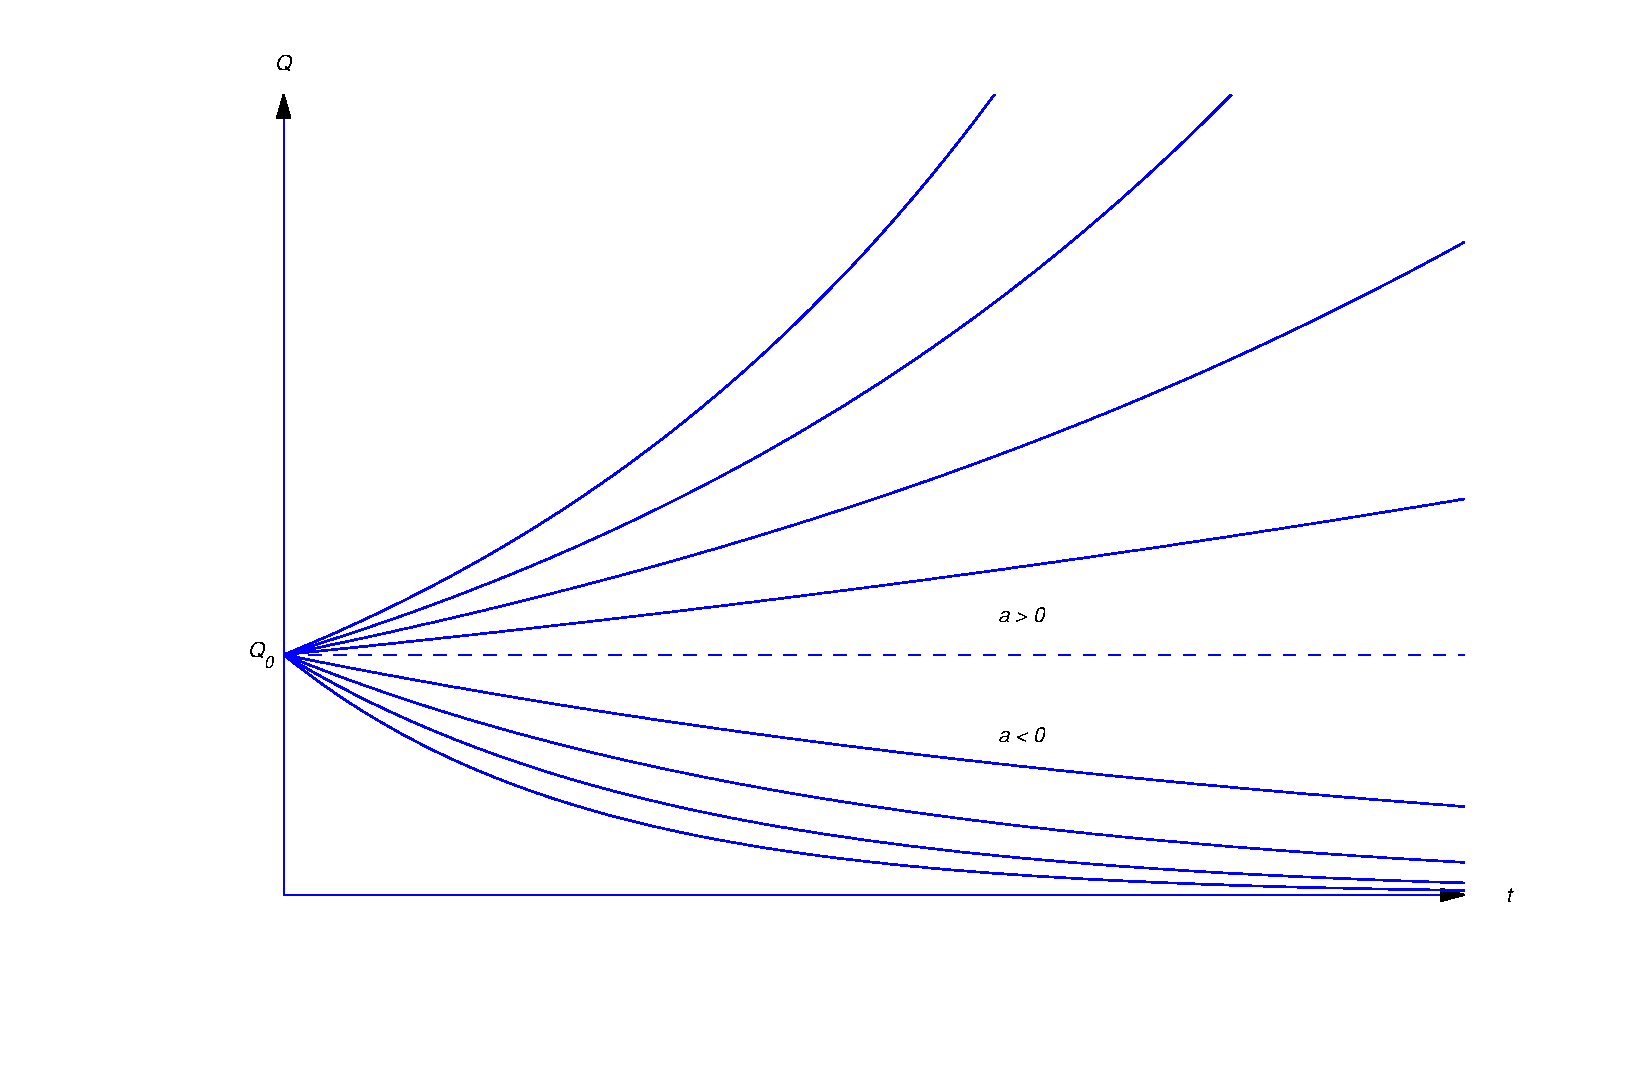
\includegraphics[bb=-78 148 689 643,width=5.67in,height=3.66in,keepaspectratio]{fig040101}
\color{blue}
\caption{\label{figure:4.1.1} Exponential growth  and decay}
  \label{figure4.1.1}
\end{figure}

\boxit{Radioactive Decay}

\noindent
Experimental evidence shows that radioactive material decays at a rate
proportional to the mass of the material present. According to this
model the mass $Q(t)$ of a radioactive material present at time $t$
satisfies \eqref{eq:4.1.1}, where $a$ is a negative constant whose value
for any given material must be determined by experimental observation.
For simplicity, we'll replace the negative constant $a$ by
$-k$, where
$k$ is a positive number that we'll call the {\color{blue}\it decay constant\/}
of the material. Thus, \eqref{eq:4.1.1} becomes
$$
Q'=-kQ.
$$
If the mass of the material present
at $t=t_0$ is $Q_0$,  the mass present at time $t$ is
 the solution of
$$
Q'=-kQ,\quad  Q(t_0)=Q_0.
$$
From \eqref{eq:4.1.2}  with $a=-k$, the solution of this initial value
problem is
\begin{equation} \label{eq:4.1.3}
Q=Q_0e^{-k(t-t_0)}.
\end{equation}

The {\color{blue}\it half--life} $\tau$ of a radioactive material is defined to be
the time required for half of its mass to decay; that is, if
$Q(t_0)=Q_0$, then \begin{equation} \label{eq:4.1.4} Q(\tau+t_0)={Q_0\over
2}.
\end{equation}
 From \eqref{eq:4.1.3} with $t=\tau+t_0$, \eqref{eq:4.1.4} is equivalent to
$$
Q_0e^{-k\tau}={Q_0\over 2},
$$
 so
$$
e^{-k\tau}={1\over 2}.
$$
 Taking logarithms  yields
$$
-k\tau=\ln{1\over 2}=-\ln2,
$$
 so the half-life is
\begin{equation} \label{eq:4.1.5}
\tau={1\over k}\ln2.
\end{equation}
(Figure \ref{figure:4.1.2}). The half-life is independent of $t_0$ and
$Q_0$, since it's determined by the properties of material, not by
the amount of the material present at any particular time.

\begin{figure}[tbp]
  \centering
  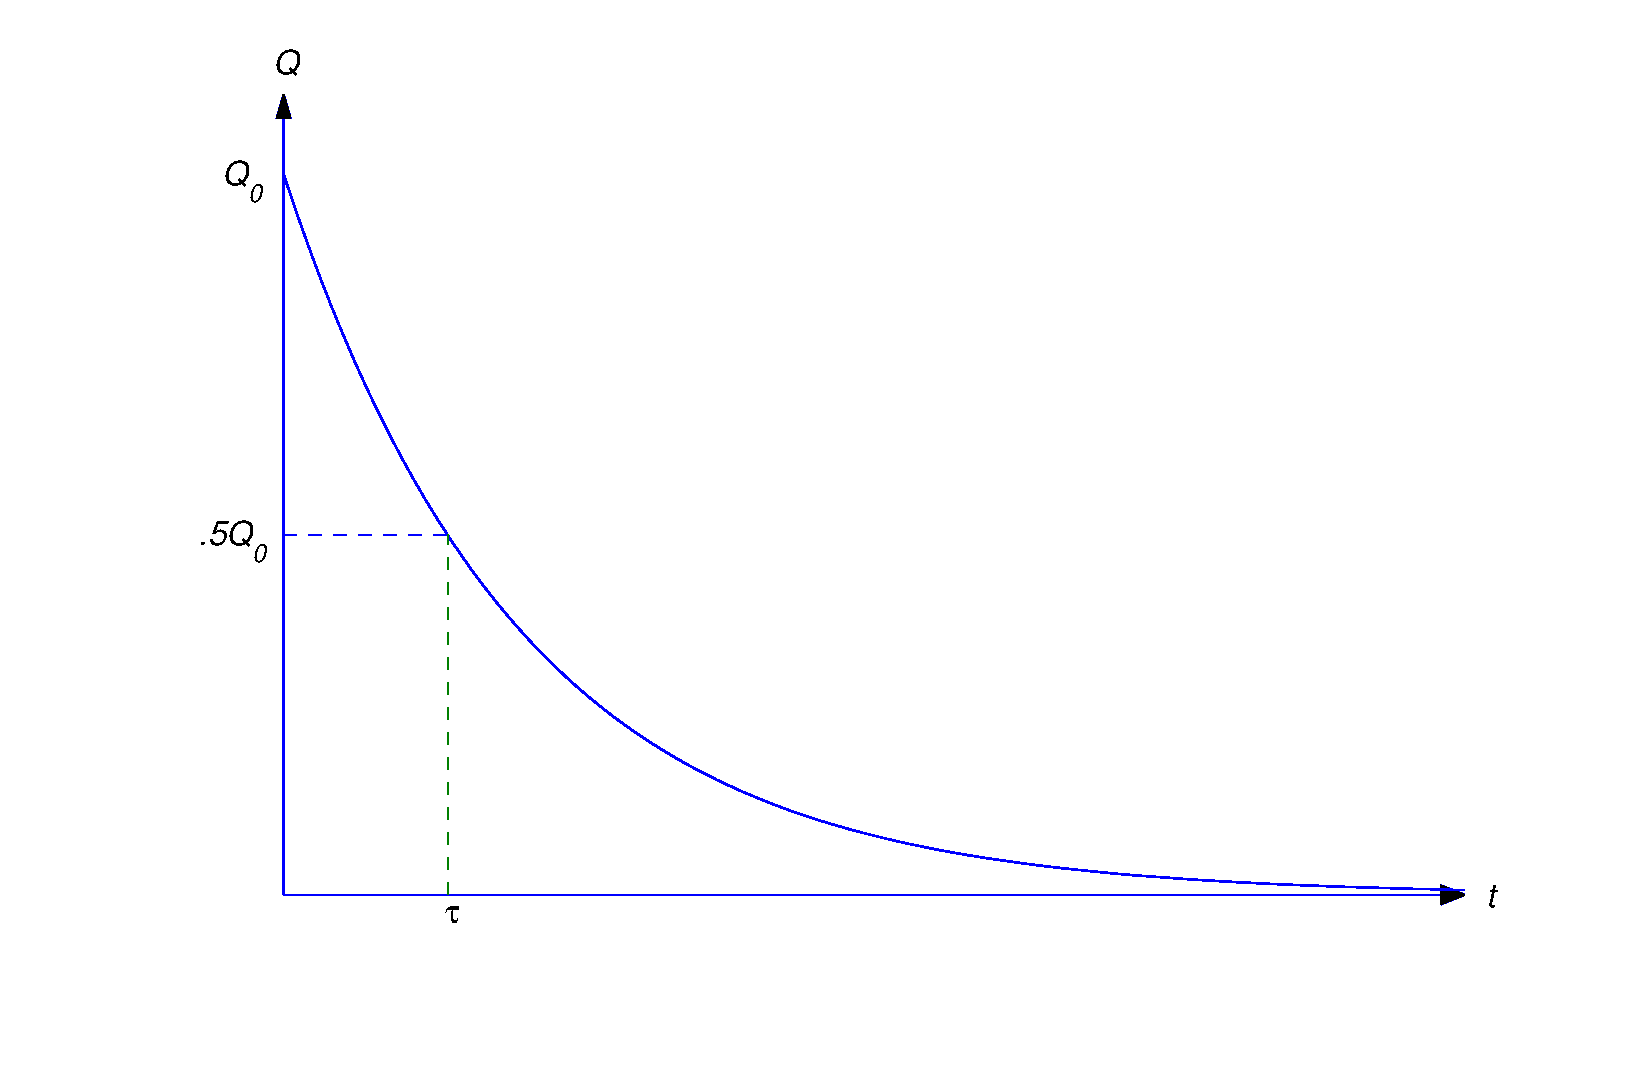
\includegraphics[bb=-78 148 689 643,width=5.67in,height=3.66in,keepaspectratio]{fig040102}
\color{blue}
\caption{Half-life of a radioactive substance}
  \label{figure:4.1.2}
\end{figure}

\begin{example}\label{example:4.1.1} \rm
A  radioactive substance has a half-life of 1620 years.
\begin{alist}
\item %(a)
If its mass is now 4 g (grams), how much will be left 810 years
from now?
\item % (b)
Find the time $t_1$ when 1.5 g of the substance remain.
\end{alist}
\end{example}

\solutionpart{a}  From \eqref{eq:4.1.3} with $t_0=0$ and
$Q_0=4$,
\begin{equation} \label{eq:4.1.6}
Q=4e^{-kt},
\end{equation}
 where we determine $k$ from \eqref{eq:4.1.5}, with $\tau$=
1620 years:
$$
k={\ln2\over\tau}={\ln2\over 1620}.
$$
 Substituting this in \eqref{eq:4.1.6} yields
\begin{equation} \label{eq:4.1.7}
Q=4e^{-(t\ln2)/1620}.
\end{equation}
 Therefore the mass left after 810 years will be
$$\begin{array}{rl}
Q(810) &=4e^{-(810\ln2)/1620}=4e^{-(\ln2)/2} \\
&=2\sqrt{2} \mbox{ g}.
\end{array}$$

\solutionpart{b}
 Setting $t=t_1$  in \eqref{eq:4.1.7} and requiring that
$Q(t_1)=1.5$ yields
$$
{3\over2}=4e^{(-t_1\ln2)/1620}.
$$
Dividing by 4 and taking logarithms yields
$$
\ln{3\over8}=-{t_1\ln2\over1620}.
$$
Since $\ln3/8=-\ln8/3$,
$$
t_1=1620{\ln8/3\over\ln2}\approx  2292.4\;\mbox{ years}.
$$

\boxit{Interest Compounded Continuously}

\noindent
Suppose we deposit an amount of money $Q_0$  in an
interest-bearing account and make no further deposits or withdrawals
for $t$ years, during which the account bears interest at a constant
annual rate $r$. To calculate the value of the account at the
end of $t$ years, we need one more piece of information: how the
interest is added to the account, or---as the bankers say---how it
is {\color{blue}\it compounded}. If the interest is compounded annually,  the
value of the account is multiplied by $1+r$ at the end of each year.
This means that after $t$ years the value of the account is
$$
Q(t)=Q_0(1+r)^t.
$$
If interest is compounded semiannually,  the
value of the account is multiplied by $(1+r/2)$ every 6 months.
Since this occurs twice annually, the value of the account after $t$
years is
$$
Q(t)=Q_0\left(1+{r\over 2}\right)^{2t}.
$$
In general, if interest is compounded $n$ times per year, the value of
the account is multiplied $n$ times per year by $(1+r/n)$;  therefore,
the value of the account
after $t$ years is
\begin{equation} \label{eq:4.1.8}
Q(t)=Q_0\left(1+{r\over n}\right)^{nt}.
\end{equation}
Thus, increasing the  frequency of  compounding increases the value of the
account after a fixed period of time. Table~\ref{table:4.1.1} shows the
effect
of increasing the number of compoundings over $t=5$ years on an initial
deposit of $Q_0=100$ (dollars), at an annual interest rate of 6\%.

\medskip

\begin{newtable} \label{table:4.1.1}
The effect of
compound interest
\begin{center}
$$\begin{array}{|c|c|}\hline
n & \dst\$100 \left(1+{.06\over n}\right)^{5n}\\
\hbox{(number of compoundings} &   \hbox{(value in dollars}\\
\hbox{per year)} &\hbox{after 5 years)}\\
\hline
1 & \$133.82 \\
2 & \$134.39 \\
4 & \$134.68 \\
8 & \$134.83 \\
364 & \$134.98 \\\hline
\end{array}$$
\end{center}
\end{newtable}

\medskip
You can see from Table~\ref{table:4.1.1}  that the value of the account after 5
years is an increasing function of $n$. Now suppose  the maximum
allowable rate of interest on savings accounts is restricted by law,
but the time intervals between successive compoundings isn't ; then
competing banks can attract savers by compounding often. The ultimate
step in this direction is to {\color{blue}\it compound continuously}, by which we
mean that $n\to\infty$ in \eqref{eq:4.1.8}. Since we know from calculus
that
$$
\lim_{n\to\infty} \left(1+{r\over n}\right)^n=e^r,
$$
 this yields
$$\begin{array}{rl}
Q(t) & \dst=\lim_{n\to\infty} Q_0\left(1+{r\over
n}\right)^{nt}=Q_0 \left[
\lim_{n\to\infty} \left(1+{r\over n}\right)^n\right]^t \\[12pt]
&=Q_0e^{rt}.
\end{array}$$
Observe that $Q=Q_0e^{rt}$ is the solution of the initial value problem
$$
Q'=rQ, \quad Q(0)=Q_0;
$$
 that is, with continuous compounding the value of the account
grows exponentially.

\begin{example}\label{example:4.1.2} \rm
If \$150 is deposited in a bank that pays
$5{1\over2}$\% annual
interest compounded continuously,  the value of the account after
$t$ years is
$$
Q(t)=150e^{.055t}
$$
dollars. (Note that it's necessary to write the interest rate as a
decimal;   thus, $r=.055$.) Therefore, after $t=10$ years the value
of the account is
$$
Q(10)=150e^{.55} \approx \$259.99.
$$
\end{example}

\begin{example}\label{example:4.1.3} \rm
We wish to accumulate \$10,000 in 10 years by making a single deposit
in a savings account bearing $5{1\over2}$\% annual interest
compounded continuously. How much must we deposit in the account?
\end{example}

\solution  The value of the account at time $t$ is
\begin{equation} \label{eq:4.1.9}
Q(t)=Q_0e^{.055t}.
\end{equation}
Since we want $Q(10)$ to be \$10,000, the initial deposit $Q_0$ must
satisfy the equation
\begin{equation} \label{eq:4.1.10}
10000=Q_0e^{.55},
\end{equation}
 obtained by setting $t=10$ and $Q(10)=10000$ in
\eqref{eq:4.1.9}.  Solving \eqref{eq:4.1.10} for $Q_0$ yields
$$
Q_0=10000e^{-.55} \approx \$5769.50.
$$

\boxit{Mixed Growth and Decay}

\begin{example}\label{example:4.1.4} \rm
A radioactive substance with decay constant $k$ is produced at a
constant rate of $a$ units of mass per unit time.
\begin{alist}
\item %(a)
Assuming that $Q(0)=Q_0$, find the mass $Q(t)$ of the
substance present at time~$t$.

\item %(b)
Find $\lim_{t\to\infty} Q(t)$.
\end{alist}
\end{example}

\solutionpart{a}  Here
$$
Q'=\mbox{ rate of increase of } Q - \mbox{ rate of decrease
of } Q.
$$
The rate of increase is the constant $a$. Since $Q$ is radioactive
with decay constant $k$, the rate of decrease is $kQ$. Therefore
$$
Q'=a-kQ.
$$
This is a linear first order differential equation. Rewriting it and
imposing the initial condition shows that $Q$ is the solution of the
initial value problem
\begin{equation}  \label{eq:4.1.11}
Q'+kQ=a, \quad Q(0)=Q_0.
\end{equation}
Since
$e^{-kt}$ is a solution of the complementary equation, the solutions
of \eqref{eq:4.1.11} are of the form $Q=ue^{-kt}$, where $u'e^{-kt}=a$, so
$u'=ae^{kt}$. Hence,
$$
u={a\over k}e^{kt}+c
$$
and
$$
Q=ue^{-kt}={a\over k}+ce^{-kt}.
$$
 Since $Q(0)=Q_0$, setting $t=0$ here yields
$$
Q_0={a\over k}+c  \mbox{\quad or \quad} c=Q_0-{a\over k}.
$$
 Therefore
\begin{equation} \label{eq:4.1.12}
Q={a\over k}+\left(Q_0-{a\over k}\right)e^{-kt}.
\end{equation}

\solutionpart{b}
Since $k > 0$,  $\lim_{t\to\infty} e^{-kt}=0$, so
from \eqref{eq:4.1.12}
$$
\lim_{t\to\infty} Q(t)={a\over k}.
$$
This limit depends only on $a$ and $k$, and not on $Q_0$.
We say that $a/k$ is the {\color{blue}\it steady state} value of $Q$. From
\eqref{eq:4.1.12} we also see that $Q$ approaches its steady state value
from above if $Q_0 > a/k$, or from below if $Q_0 < a/k$. If $Q_0=a/k$,
then $Q$ remains constant (Figure \ref{figure:4.1.3}).

\begin{figure}[tbp]
  \centering
  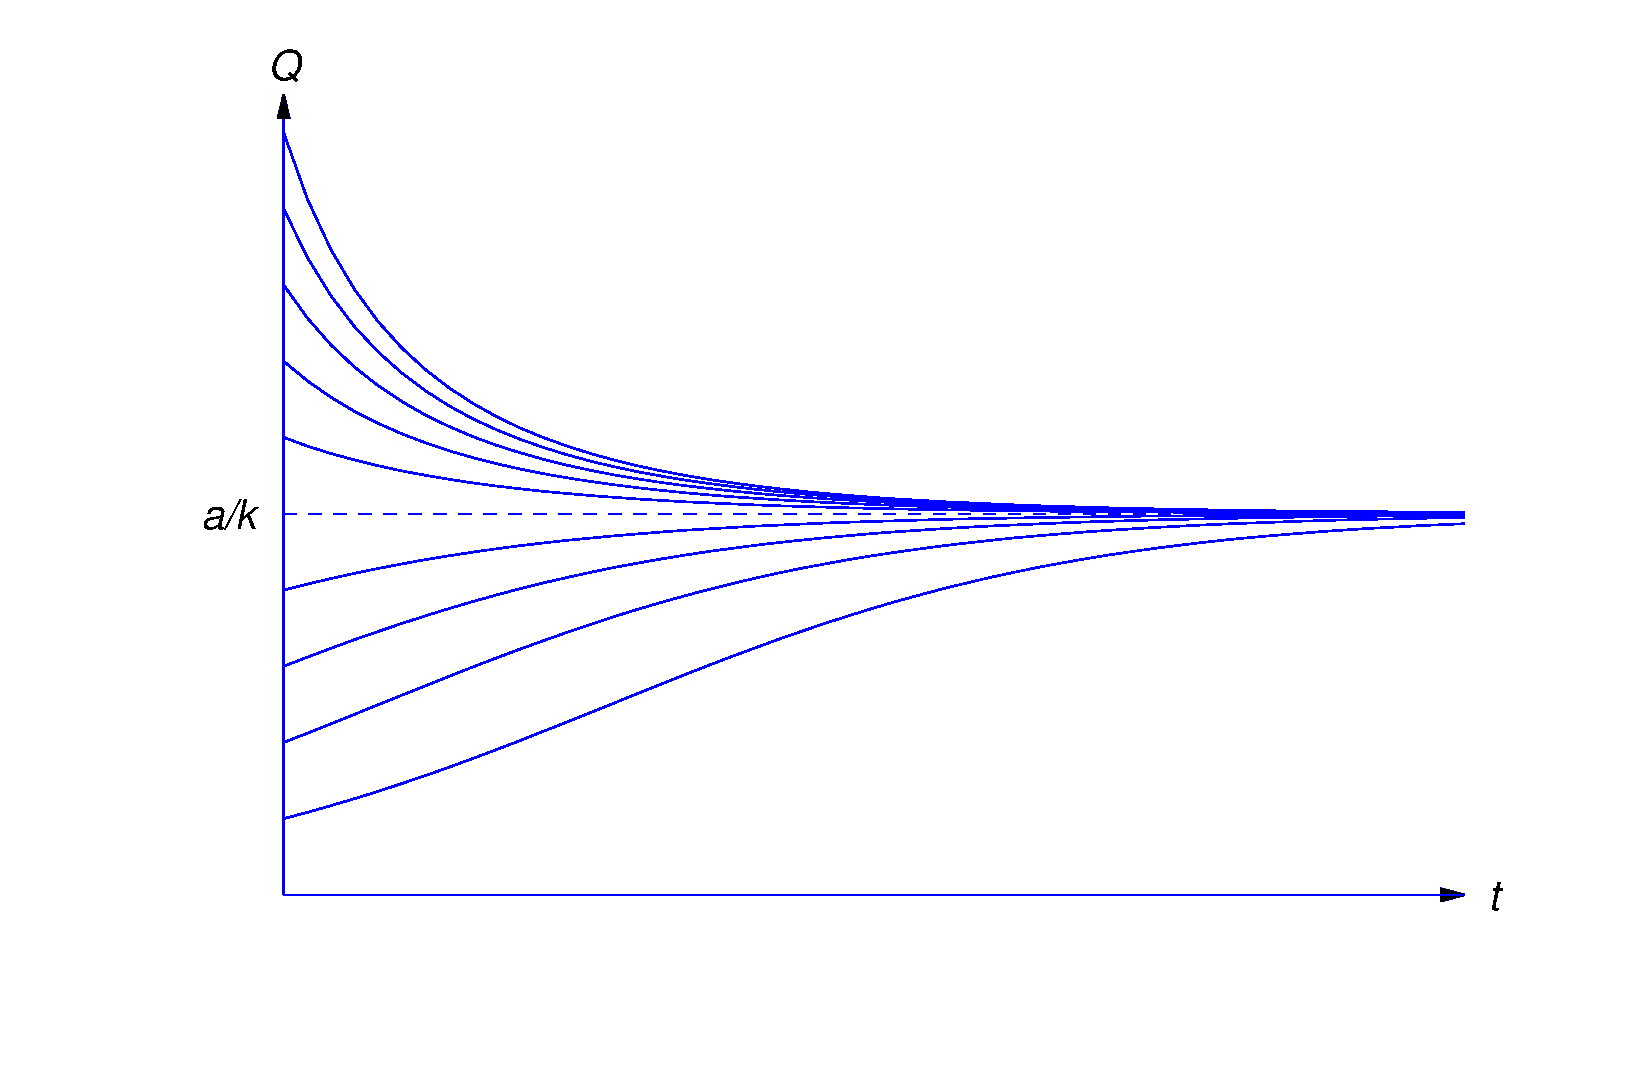
\includegraphics[bb=-78 148 689 643,width=5.67in,height=3.66in,keepaspectratio]{fig040103}
\color{blue}
\caption{$Q(t)$ approaches the steady state value
$\dst{a\over k}$ as $t\to\infty$}
  \label{figure:4.1.3}
\end{figure}

\boxit{Carbon Dating}

\noindent
The fact that $Q$ approaches a steady state value in the
situation discussed in Example 4 underlies the method of {\color{blue}\it carbon
dating}, devised by  the American chemist  and Nobel Prize Winner
\href{https://www.nobelprize.org/uploads/2018/06/libby-lecture.pdf}
{\color{blue}\it W.S. Libby}.

Carbon 12 is stable, but carbon-14, which is produced by cosmic
bombardment of nitrogen in the upper atmosphere, is radioactive with a
half-life of about 5570 years. Libby assumed that the
quantity
of carbon-12 in the atmosphere has been constant throughout time, and
that the quantity of radioactive carbon-14 achieved its steady state
value long ago as a result of its creation and decomposition over
millions of years. These assumptions led Libby to conclude that the
ratio of carbon-14 to carbon-12 has been nearly constant for a long
time. This constant, which we denote by $R$, has been determined
experimentally.

Living cells absorb both carbon-12 and carbon-14 in the proportion in
which they are present in the environment. Therefore the ratio of
carbon-14 to carbon-12 in a living cell is always $R$. However, when
the cell dies it ceases to absorb carbon, and the ratio of carbon-14
to carbon-12 decreases exponentially as the radioactive carbon-14
decays. This is the basis for the method of carbon dating, as
illustrated in the next example.

\begin{example}\label{example:4.1.5} \rm
An archaeologist investigating the site of an ancient village finds a
burial ground where the amount of carbon-14 present in individual
remains is between 42 and 44\% of the amount present in live
individuals. Estimate the age of the village and the length of time
for which it survived.
\end{example}

\solution Let $Q=Q(t)$ be the quantity of carbon-14 in an individual
set of remains $t$ years after death, and let $Q_0$ be the quantity
that would be present in  live individuals.
Since carbon-14 decays exponentially with half-life 5570 years, its
decay constant is
$$
k={\ln2\over 5570}.
$$
 Therefore
$$
Q=Q_0e^{-t(\ln2)/5570}
$$
 if we choose our time scale so that $t_0=0$ is the
time of death.  If we know the present value of $Q$  we
can solve this equation for $t$, the number of years since
death occurred.  This yields
$$
t=-5570 {\ln Q/Q_0\over\ln2}.
$$
It is given that $Q=.42Q_0$ in the remains of individuals who died
first. Therefore these deaths occurred about
$$
t_1=-5570 {\ln .42\over\ln2} \approx 6971
$$
 years ago.  For the most recent deaths, $Q=.44
Q_0$; hence, these deaths occurred about
$$
t_2=-5570 {\ln .44\over\ln2} \approx 6597
$$
 years ago.  Therefore it's reasonable to conclude
that the village was founded about 7000 years ago,
and lasted for about 400 years.

\boxit{A Savings Program}

\vspace*{-.2in}
\noindent
\begin{example}\label{example:4.1.6} \rm
A person opens a savings account with an initial deposit of \$1000 and
subsequently deposits \$50 per week. Find the value $Q(t)$ of the
account at time $t > 0$, assuming that the bank pays 6\%
interest compounded continuously.
\end{example}

\solution Observe that $Q$ isn't  continuous, since there are 52
discrete deposits per year of \$50 each. To construct a mathematical
model for this problem in the form of a differential equation, we make
the simplifying assumption that the deposits are made continuously at
a rate of \$2600 per year. This is essential, since solutions of
differential equations are continuous functions. With this assumption,
$Q$ increases continuously at the rate
$$
Q'=2600+.06 Q
$$
and therefore $Q$ satisfies the differential equation
\begin{equation} \label{eq:4.1.13}
Q'-.06Q=2600.
\end{equation}
(Of course, we must recognize that the solution of this equation
is an approximation to the true value of $Q$ at any given time. We'll
discuss this further below.)  Since $e^{.06t}$ is a solution of the
complementary equation, the solutions of \eqref{eq:4.1.13}  are of the
form   $Q=ue^{.06t}$,  where $u'e^{.06t}=2600$. Hence,
$u'=2600e^{-.06t}$,
$$
u=- {2600\over .06}e^{-.06t}+c
$$
and
\begin{equation} \label{eq:4.1.14}
Q=ue^{.06t}=-{2600\over .06}+ce^{.06t}.
\end{equation}
 Setting $t=0$ and $Q=1000$ here yields
$$
c=1000+{2600\over .06},
$$
and substituting this into \eqref{eq:4.1.14} yields
\begin{equation} \label{eq:4.1.15}
Q=1000e^{.06t}+{2600\over .06}(e^{.06t}-1),%\tag15
\end{equation}
where the first term is the value due to the initial deposit and the
second is due to the subsequent weekly deposits. \bbox

Mathematical models must be tested for validity by comparing
predictions based on them with the actual outcome of experiments.
Example 6 is unusual in that we can compute the exact value of the
account at any specified time and compare it with the approximate
value predicted by \eqref{eq:4.1.15} (See Exercise \ref{exer:4.1.21}.). The
follwing table
 gives a comparison for a ten year period. Each exact answer
corresponds to the time of the year-end deposit, and each year is
assumed to have exactly 52 weeks.

$$
\vbox{\tabskip=0pt \offinterlineskip
\def\tablerule{\noalign{\hrule}}
\halign{\hfill#\hfill&\qquad\hfill#\hfill&\qquad\hfill#\hfill
  &\qquad\hfill#\hfill&\qquad#\hfill\cr
%\noalign{\centerline{\bf Table \label{table:4.1.2}}}
\noalign{\vskip12pt}
%\noalign{\centerline{Value of the Saver's Account (Example
%\ref{example:4.1.6})}}
\noalign{\vskip22pt}
Year & Approximate Value of $Q$ & Exact Value of  $P$ & Error & Percentage
Error
\cr & (Example~\ref{example:4.1.6}) & (Exercise~\ref{exer:4.1.21}) & $Q-P$ &\ \;
$(Q-P)/P$ \cr \noalign{\vskip16pt}
\  1 & \$ 3741.42 & \$ 3739.87 & \$ 1.55 &\ \; $.0413 $\% \cr
\noalign{\vskip7pt}
\  2 &\  \, 6652.36 &\ \;  6649.17 &\ \; 3.19 &\ \; $.0479$
\cr
\noalign{\vskip7pt}
\  3 &\  \, 9743.30 &\ \;  9738.37 &\ \; 4.93 &\ \; $.0506$
\cr
\noalign{\vskip7pt}
\  4 & \, 13,025.38 & \, 13,018.60 &\ \; 6.78 &\ \; $.0521$
\cr
\noalign{\vskip7pt}
\  5 & \, 16,510.41 & \, 16,501.66 &\ \; 8.75 &\ \; $.0530 $
\cr
\noalign{\vskip7pt}
\  6 & \, 20,210.94 & \, 20,200.11 & 10.83 &\ \; $.0536$
\cr
\noalign{\vskip7pt}
\  7 & \, 24,140.30 & \, 24,127.25 & 13.05 &\ \; $.0541 $
\cr
\noalign{\vskip7pt}
\  8 & \, 28,312.63 & \, 28,297.23 & 15.40 &\ \; $.0544 $
\cr
\noalign{\vskip7pt}
\  9 & \, 32,742.97 & \, 32,725.07 & 17.90 &\ \; $.0547 $
\cr
\noalign{\vskip7pt}
10 & \, 37,447.27 & \, 37,426.72 & 20.55 &\ \; $.0549 $ \cr}}
$$
\newpage

\exercises

\begin{exerciselist}
\item\label{exer:4.1.1}
The half-life of a radioactive substance is 3200
years.  Find the quantity $Q(t)$ of the substance left at
time $t > 0$ if $Q(0)=20$ g.

\item\label{exer:4.1.2}
The half-life of a radioactive substance is 2 days.  Find
the time required for a given amount of the material to
decay to 1/10 of its original mass.

\item\label{exer:4.1.3}
A  radioactive material loses 25\% of its mass
in 10 minutes.  What is its half-life?

\item\label{exer:4.1.4}
A  tree contains a known percentage $p_0$ of
a radioactive substance with half-life $\tau$.  When the
tree dies the substance decays and isn't  replaced.  If the
percentage of the substance in the fossilized remains of
such a tree is found to be $p_1$, how long has the tree been
dead?

\item\label{exer:4.1.5}
If $t_p$ and $t_q$ are the times required for a radioactive
material to decay to $1/p$ and $1/q$  times
its original mass (respectively), how are $t_p$ and $t_q$ related?

\item\label{exer:4.1.6}
Find the decay constant $k$ for a radioactive substance,
given that the mass of the substance is $Q_1$ at time $t_1$
and $Q_2$ at time $t_2$.

\item\label{exer:4.1.7}
A process creates a radioactive substance at the rate of 2
g/hr and the substance decays at a rate proportional to
its mass, with constant of proportionality
$k=.1 (\mbox{hr})^{-1}$.  If $Q(t)$ is the mass of the
substance at time $t$, find $\lim_{t\to\infty}Q(t)$.

\item\label{exer:4.1.8}
A bank pays interest continuously at the rate of 6\%.
How long does it take for a deposit of $Q_0$ to grow in
value to $2Q_0$?

\item\label{exer:4.1.9}
At what rate of interest, compounded continuously, will a
bank deposit double in value in 8 years?

\item\label{exer:4.1.10}
A savings account pays 5\% per annum interest compounded
continuously. The initial deposit is $Q_0$ dollars. Assume that there
are no subsequent withdrawals or deposits.
\begin{alist}
\item % (a)
How long will it take for the value of the account to triple?
\item % (b)
What is $Q_0$ if the value of the account after 10 years is \$100,000
dollars?
\end{alist}

\item\label{exer:4.1.11}
A candymaker makes 500 pounds of candy per week, while
his large family eats the candy at a rate equal to $Q(t)/10$
pounds per week, where $Q(t)$ is the amount of candy present
at time $t$.
\begin{alist}
\item %(a)
Find $Q(t)$ for $t > 0$ if the candymaker has 250 pounds of
candy at $t=0$.
\item %(b)
Find $\lim_{t\to\infty} Q(t)$.
\end{alist}

\item\label{exer:4.1.12}
Suppose a substance decays at a yearly rate  equal
to half the square of the mass of the substance present.  If
we start with 50 g of the substance, how long will it be
until only 25 g remain?

\item\label{exer:4.1.13}
A super bread dough increases in volume at a rate
proportional to the volume $V$ present.  If $V$ increases by
a factor of 10 in 2 hours and $V(0)=V_0$, find $V$ at any
time $t$.  How long will it take for $V$ to increase to $100
V_0$?

\item\label{exer:4.1.14}
A radioactive substance decays at a rate proportional to the
amount present, and half the original quantity $Q_0$ is left
after 1500 years. In how many years would the original
amount be reduced to $3Q_0/4$?  How much will be
left after 2000 years?

\item\label{exer:4.1.15}
A wizard creates gold continuously at the rate of 1 ounce
per hour, but an assistant steals it continuously at the
rate of 5\% of however much  is there per hour.  Let $W(t)$
be the number of ounces that the wizard has at time $t$.
Find $W(t)$ and $\lim_{t\to\infty}W(t)$ if  $W(0)=1$.

\item\label{exer:4.1.16}
A process creates a radioactive substance at the rate of 1
g/hr, and the substance decays at an hourly rate
 equal to 1/10 of the mass present (expressed in
grams).  Assuming that there are initially 20 g, find
the mass $S(t)$ of the substance present at time $t$, and
find $\lim_{t\to\infty} S(t)$.

\item\label{exer:4.1.17}
A tank is empty at $t=0$.  Water is added to the tank at
the rate of 10 gal/min, but it leaks out at a rate
 (in gallons per minute)  equal to the number of
gallons in the tank.  What is the smallest capacity the tank
can have if this process is to continue forever?

\item\label{exer:4.1.18}
A person deposits \$25,000 in a bank that pays 5\% per
year interest, compounded continuously.  The person
continuously withdraws from the account at the rate of \$750
per year.  Find $V(t)$, the value of the account at time $t$
after the initial deposit.

\item\label{exer:4.1.19}
  A person has a fortune that grows at rate proportional to the
square root of its worth. Find the  worth $W$ of the fortune as a function
of $t$ if it was  \$1 million 6 months ago and
is \$4 million today.

\item\label{exer:4.1.20}
Let $p=p(t)$ be the quantity of a  product present at
time $t$. The product is manufactured continuously at a
rate proportional to $p$, with proportionality constant 1/2,
and it's consumed continuously at a rate proportional to
$p^2$, with proportionality constant 1/8.  Find $p(t)$ if
$p(0)=100$.

\item\label{exer:4.1.21}

\begin{alist}
\item % (a)
 In the situation of Example~\ref{example:4.1.6}
find the exact value $P(t)$ of the person's account after $t$
years, where $t$ is an integer.  Assume that each year has
exactly 52 weeks, and include the year-end
deposit in the computation.

\hint{At time $t$ the initial $\$1000$
has been on deposit for $t$ years.  There have been $52t$
deposits of $\$50$ each.  The first $\$50$ has been on deposit
for $t-1/52$ years, the second for $t-2/52$ years $\cdots$
in general, the $j$th $\$50$ has been on deposit for $t-j/52$
years $(1 \le j \le 52t)$.  Find the present value of each
$\$50$ deposit assuming $6$\% interest compounded
continuously, and use the formula
$$
1+x+x^2+\cdots+x^n={1-x^{n+1}\over 1-x}\
(x \ne 1)
$$
to find their total value.}

\item % (b)
 Let
$$
p(t)={Q(t)-P(t)\over P(t)}
$$
be the relative error after $t$ years.  Find
$$
p(\infty)=\lim_{t\to\infty}p(t).
$$
\end{alist}

\item\label{exer:4.1.22}
A homebuyer borrows $P_0$ dollars at an annual interest rate $r$,
agreeing to repay the loan with equal monthly payments of $M$ dollars
per month over $N$ years.
\begin{alist} \item % (a)
Derive a
differential equation for the loan principal (amount that the
homebuyer owes) $P(t)$ at time $t>0$, making the simplifying
assumption that the homebuyer repays the loan continuously rather than
in discrete steps. (See Example~\ref{example:4.1.6} .)

\item %(b)
Solve the equation derived in \part{a}.

\item % (c)
 Use the result of \part{b} to determine an approximate
value for $M$  assuming that each year has exactly 12 months of
equal length.

\item % (d)
 It can be shown that the exact value of $M$  is given by
$$
M={rP_0\over 12}\left(1-(1+r/12)^{-12N}\right)^{-1}.
$$
Compare    the value of $M$ obtained from the answer in \part{c} to the
exact value  if
 (i) $P_0=\$50,000$, $r=7{1\over2}$\%, $N=20$
 (ii) $P_0=\$150,000$, $r=9.0$\%, $N=30$.
\end{alist}

\item\label{exer:4.1.23}
Assume that the homebuyer of Exercise \ref{exer:4.1.22} elects to repay the
loan continuously at the rate of $\alpha M$ dollars per month,
where $\alpha$ is a constant greater than 1. (This is called {\color{blue}\it
accelerated payment\/}.)
\begin{alist}
\item % (a)
 Determine the time $T(\alpha)$ when the loan
will be paid off and the amount $S(\alpha)$ that the homebuyer will save.

\item % (b)
 Suppose $P_0=\$50,000$, $r=8$\%, and $N=15$.
Compute
the savings realized by accelerated payments with $\alpha=1.05,1.10$, and
$1.15$.
\end{alist}

\item\label{exer:4.1.24} A benefactor wishes to establish a trust fund to
pay a researcher's salary for $T$ years. The salary is to start at
$S_0$ dollars per year and increase at a fractional rate of $a$ per
year. Find the amount of money $P_0$ that the benefactor must deposit
in a trust fund paying interest at a rate $r$ per year. Assume that
the researcher's salary is paid continuously, the interest is
compounded continuously, and the salary increases are granted
continuously.

\item\label{exer:4.1.25} \Lex
A radioactive substance with decay constant $k$ is produced
at the rate of
$$
{at\over1+btQ(t)}
$$
 units of mass per unit time, where
$a$ and $b$ are positive constants and $Q(t)$ is the mass of the
substance present at time $t$;   thus, the rate of production is small
at the start
 and tends to slow when $Q$ is large.
\begin{alist}
\item % (a)
Set up a differential equation for $Q$.
\item % (b)
Choose your own positive values for $a$, $b$, $k$, and
$Q_0=Q(0)$.
Use a numerical method
to discover what happens to $Q(t)$
as $t\to\infty$. (Be precise, expressing your conclusions in terms of
$a$, $b$, $k$. However,  no proof is required.)
\end{alist}

\item\label{exer:4.1.26} \Lex
Follow the instructions of Exercise~\ref{exer:4.1.25}, assuming that
the substance is produced at the rate of   $at/(1+bt(Q(t))^2)$
units of mass per unit of time.

\item\label{exer:4.1.27} \Lex
Follow the instructions of Exercise~\ref{exer:4.1.25}, assuming that
the substance is produced at the rate of   $at/(1+bt)$
units of mass per unit of time.

\end{exerciselist}


\section{Cooling and Mixing}

\boxit{Newton's Law of Cooling}

\noindent
Newton's law of cooling states that if an object with temperature
$T(t)$ at time $t$ is in a medium with temperature $T_m(t)$,  the
rate of change of $T$ at time $t$ is proportional to $T(t)-T_m(t)$;
thus,
$T$ satisfies a differential equation of the form
\begin{equation} \label{eq:4.2.1}
T'=-k(T-T_m).
\end{equation}
 Here $k > 0$, since the temperature of the object must decrease if
$T > T_m$, or increase if $T < T_m$.  We'll call $k$  the {\color{blue}\it
temperature decay constant of the medium\/}.

For simplicity, in this section we'll assume  that the medium is
maintained at a constant temperature $T_m$. This is another example of
 building a simple mathematical model for a physical
phenomenon. Like most mathematical models it has its limitations. For
example, it's reasonable to assume that the temperature of a room
remains approximately constant if the cooling object is a cup of
coffee, but perhaps not if it's a huge cauldron of molten metal. (For
more on this see Exercise~\ref{exer:4.2.17}.)

To solve  \eqref{eq:4.2.1}, we rewrite it as
$$
T'+kT=kT_m.
$$
Since $e^{-kt}$ is a solution of the complementary equation, the
solutions of this equation are of the form $T=ue^{-kt}$, where
$u'e^{-kt}=kT_m$, so $u'=kT_me^{kt}$. Hence,
$$
u=T_me^{kt}+c,
$$
so
$$
T=ue^{-kt}=T_m+ce^{-kt}.
$$
If $T(0)=T_0$,  setting $t=0$ here yields $c=T_0-T_m$, so
\begin{equation} \label{eq:4.2.2}
T=T_m+(T_0-T_m)e^{-kt}.
\end{equation}
Note that $T-T_m$ decays exponentially, with decay constant $k$.

\begin{example}\label{example:4.2.1}\rm
A ceramic insulator is baked at $400^\circ$C and cooled in a room in
which the temperature is $25^\circ$C. After 4 minutes the
temperature of the insulator is $200^\circ$C. What is its temperature
after 8 minutes?
\end{example}

\solution Here $T_0=400$ and $T_m=25$, so \eqref{eq:4.2.2} becomes
\begin{equation} \label{eq:4.2.3}
T=25+375e^{-kt}.
\end{equation}
 We determine $k$ from the stated condition that  $T(4)=200$;
that is,
$$
200=25+375e^{-4k};
$$
 hence,
$$
e^{-4k} = {175\over 375} = {7\over 15}.
$$
 Taking logarithms and solving for $k$ yields
$$
k=-{1\over 4} \ln {7\over 15}={1\over 4}\ln {15\over 7}.
$$
 Substituting this into \eqref{eq:4.2.3} yields
$$
T=25+375 e^{-{t\over 4} \ln {15\over 7}}
$$
(Figure~\ref{figure:4.2.1}).
Therefore the temperature of the insulator after
8 minutes is
$$\begin{array}{rl}
T(8) & \dst = 25+375 e^{-2 \ln {15\over 7}} \\[9pt]
& \dst = 25+375 \left({7\over 15}\right)^2 \approx
107^\circ \mbox{C}.
\end{array}$$

\begin{figure}[tbp]
  \centering
  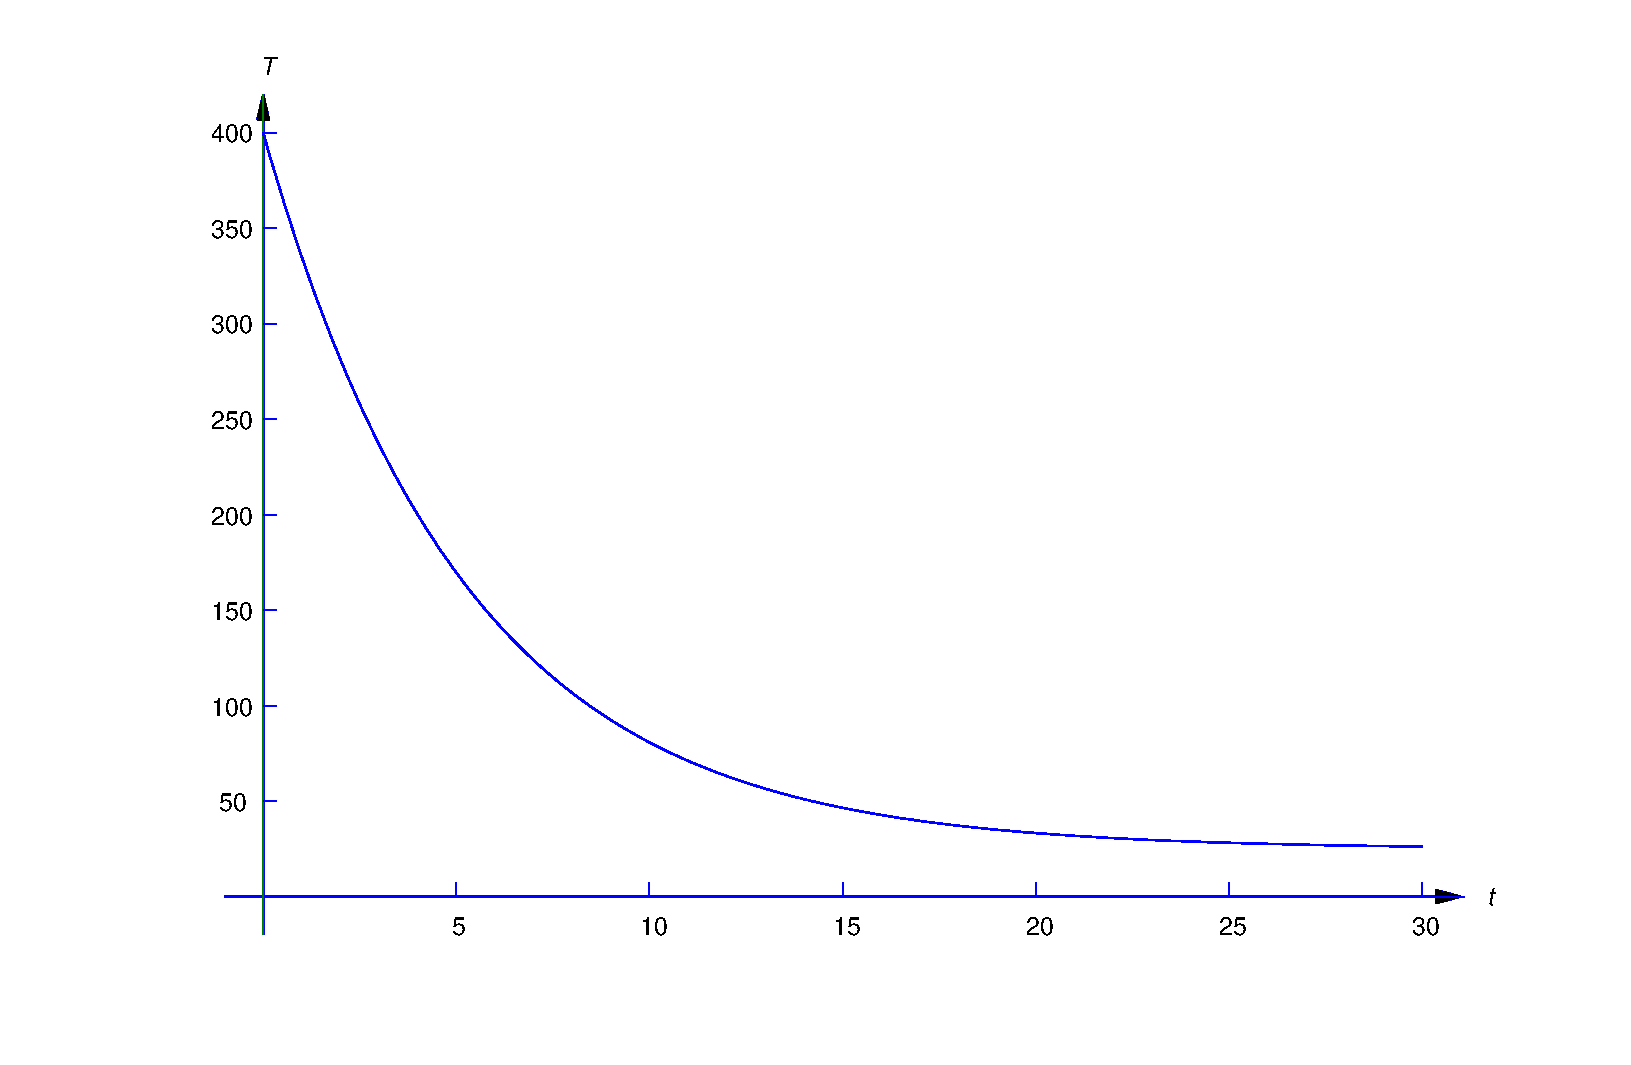
\includegraphics[bb=-78 148 689 643,width=5.67in,height=3.66in,keepaspectratio]{fig040201}
\color{blue}
\caption{$T=25+375e^{-(t/4)\ln 15/7}$}
  \label{figure:4.2.1}
\end{figure}

\begin{example}\label{example:4.2.2}\rm
An object with temperature $72^\circ$F is placed outside, where the
temperature is $-20^\circ$F. At 11:05 the temperature of the object
is $60^\circ$F and at 11:07 its temperature is $50^\circ$F. At what
time was the object placed outside?
\end{example}

\solution Let $T(t)$ be the temperature of the object at time $t$. For
convenience, we choose the origin $t_0=0$ of the time scale to be
11:05 so that $T_0=60$. We must determine the time $\tau$ when
$T(\tau)=72$. Substituting $T_0=60$ and $T_m=-20$ into \eqref{eq:4.2.2}
yields
$$
T  = -20+\bigl(60-(-20)\bigr)e^{-kt}
$$
 or
\begin{equation} \label{eq:4.2.4}
T = -20+80e^{-kt}.
\end{equation}
We obtain $k$ from the stated condition that the temperature of the
object is 50$^\circ$F at 11:07. Since 11:07 is $t=2$ on our time
scale, we can determine $k$ by substituting $T=50$ and $t=2$ into
\eqref{eq:4.2.4} to obtain
$$
50 = -20+80e^{-2k}
$$
(Figure~\ref{figure:4.2.2});
 hence,
$$
e^{-2k}={70\over 80}={7\over 8}.
$$
 Taking logarithms and solving for $k$ yields
$$
k =-{1\over 2} \ln {7\over 8} = {1\over 2} \ln {8\over 7}.
$$
 Substituting this into \eqref{eq:4.2.4} yields
$$
T = -20+80 e^{-{t\over 2}\ln {8\over 7}},
$$
 and the condition $T(\tau)=72$  implies that
$$
72 =-20+80 e^{-{\tau\over 2} \ln {8\over 7}};
$$
 hence,
$$
e^{-{\tau\over 2} \ln {8\over 7}} ={92\over 80} =
{23\over 20}.
$$
Taking logarithms and solving for $\tau$ yields
$$
\tau = -{2 \ln {23\over 20}\over \ln {8\over 7}} \approx-2.09\
\mbox{min}.
$$
Therefore the object was placed outside
about 2 minutes and 5 seconds before 11:05; that is,
at 11:02:55.

\begin{figure}[tbp]
  \centering
  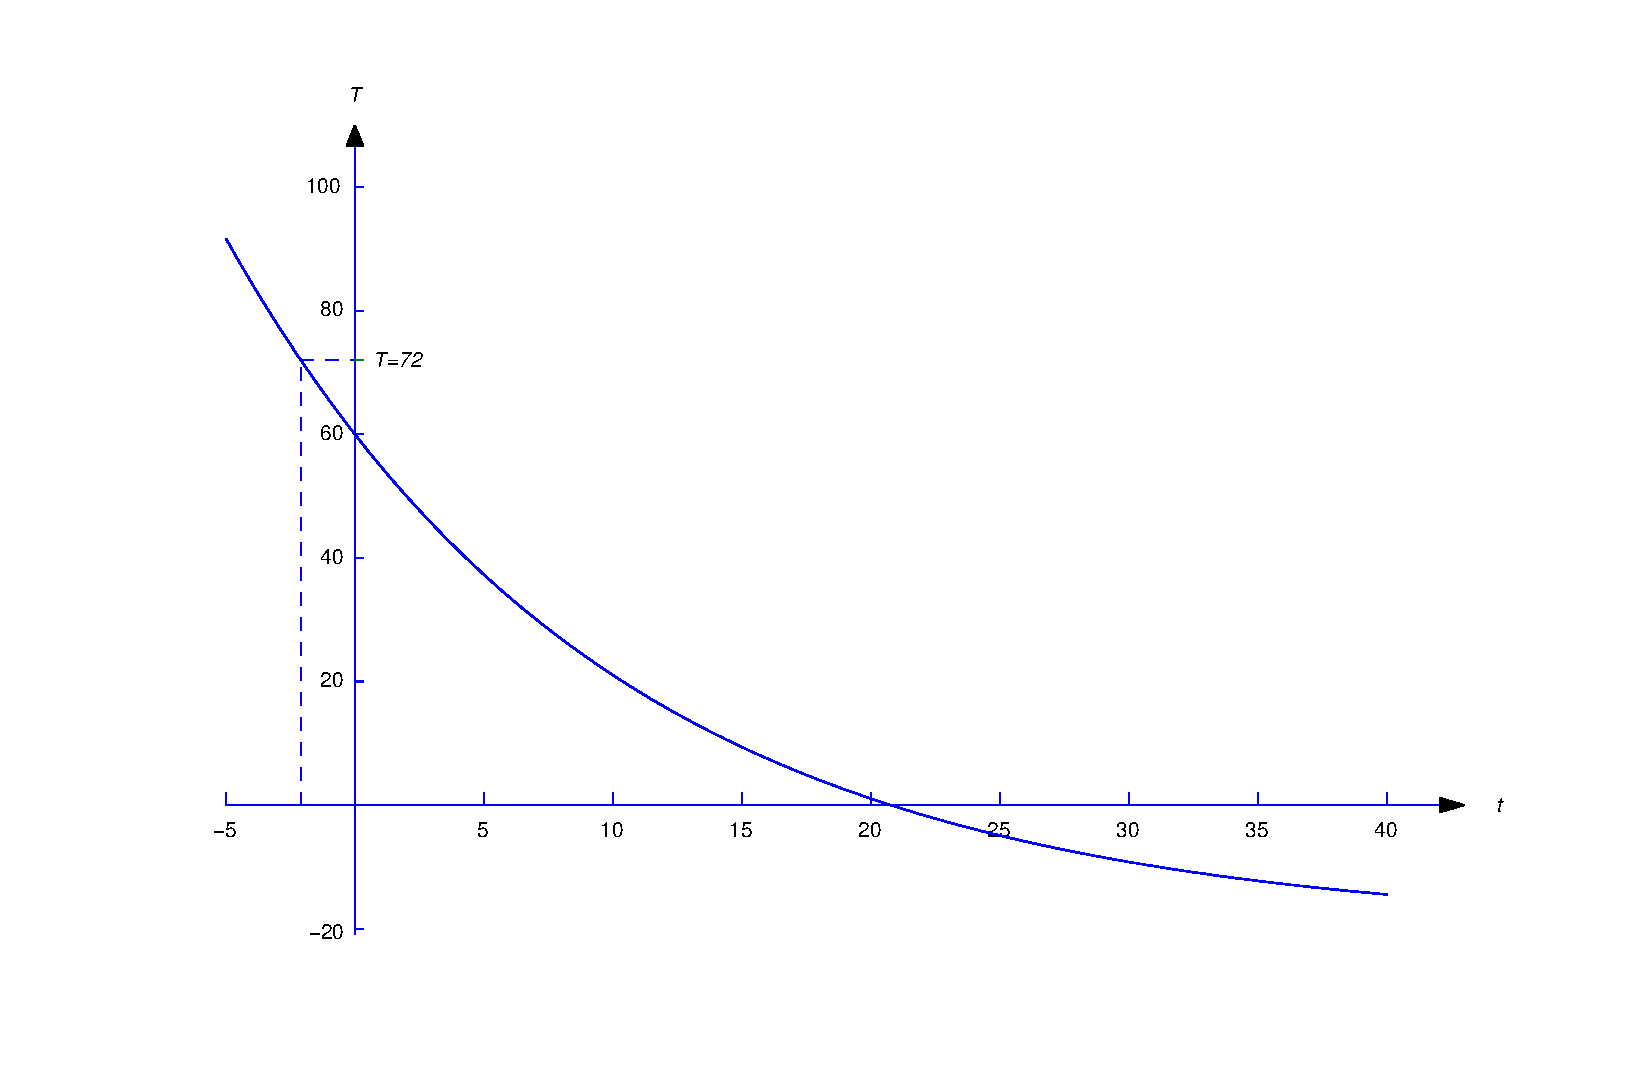
\includegraphics[bb=-78 148 689 643,width=5.67in,height=3.66in,keepaspectratio]{fig040202}
\color{blue}
  \caption{$T = -20+80 e^{-{t\over 2}\ln {8\over 7}}$}
  \label{figure:4.2.2}
\end{figure}

\boxit{Mixing Problems}

\noindent
In the next two examples a saltwater solution with a given
concentration (weight of salt per unit volume of solution) is added at
a specified rate to a tank that initially contains saltwater with a
different concentration. The problem is to determine the quantity of
salt in the tank as a function of time. This is an example of a {\color{blue}\it
mixing problem\/}. To construct a tractable mathematical model for
mixing problems we assume in our examples (and most exercises) that
the mixture is stirred instantly so that the salt is always uniformly
distributed throughout the mixture. Exercises~\ref{exer:4.2.22}
and \ref{exer:4.2.23} deal with situations where this isn't  so, but
the distribution of salt becomes approximately uniform as
$t\to\infty$.

\begin{example}\label{example:4.2.3}  \rm
A tank initially contains 40 pounds of salt dissolved in 600 gallons
of water. Starting at $t_0 = 0$, water that contains 1/2 pound of salt
per gallon is poured into the tank at the rate of 4 gal/min and the
mixture is drained from the tank at the same rate
(Figure~\ref{figure:4.2.3}).
\begin{alist}
\item % (a)
Find a differential equation for the quantity $Q(t)$ of salt in the
tank at time $t > 0$, and solve the equation to determine $Q(t)$.
\item % (b)
 Find $\lim_{t\to\infty}Q(t)$.
\end{alist}
\end{example}

\begin{figure}[tbp]
  \centering
  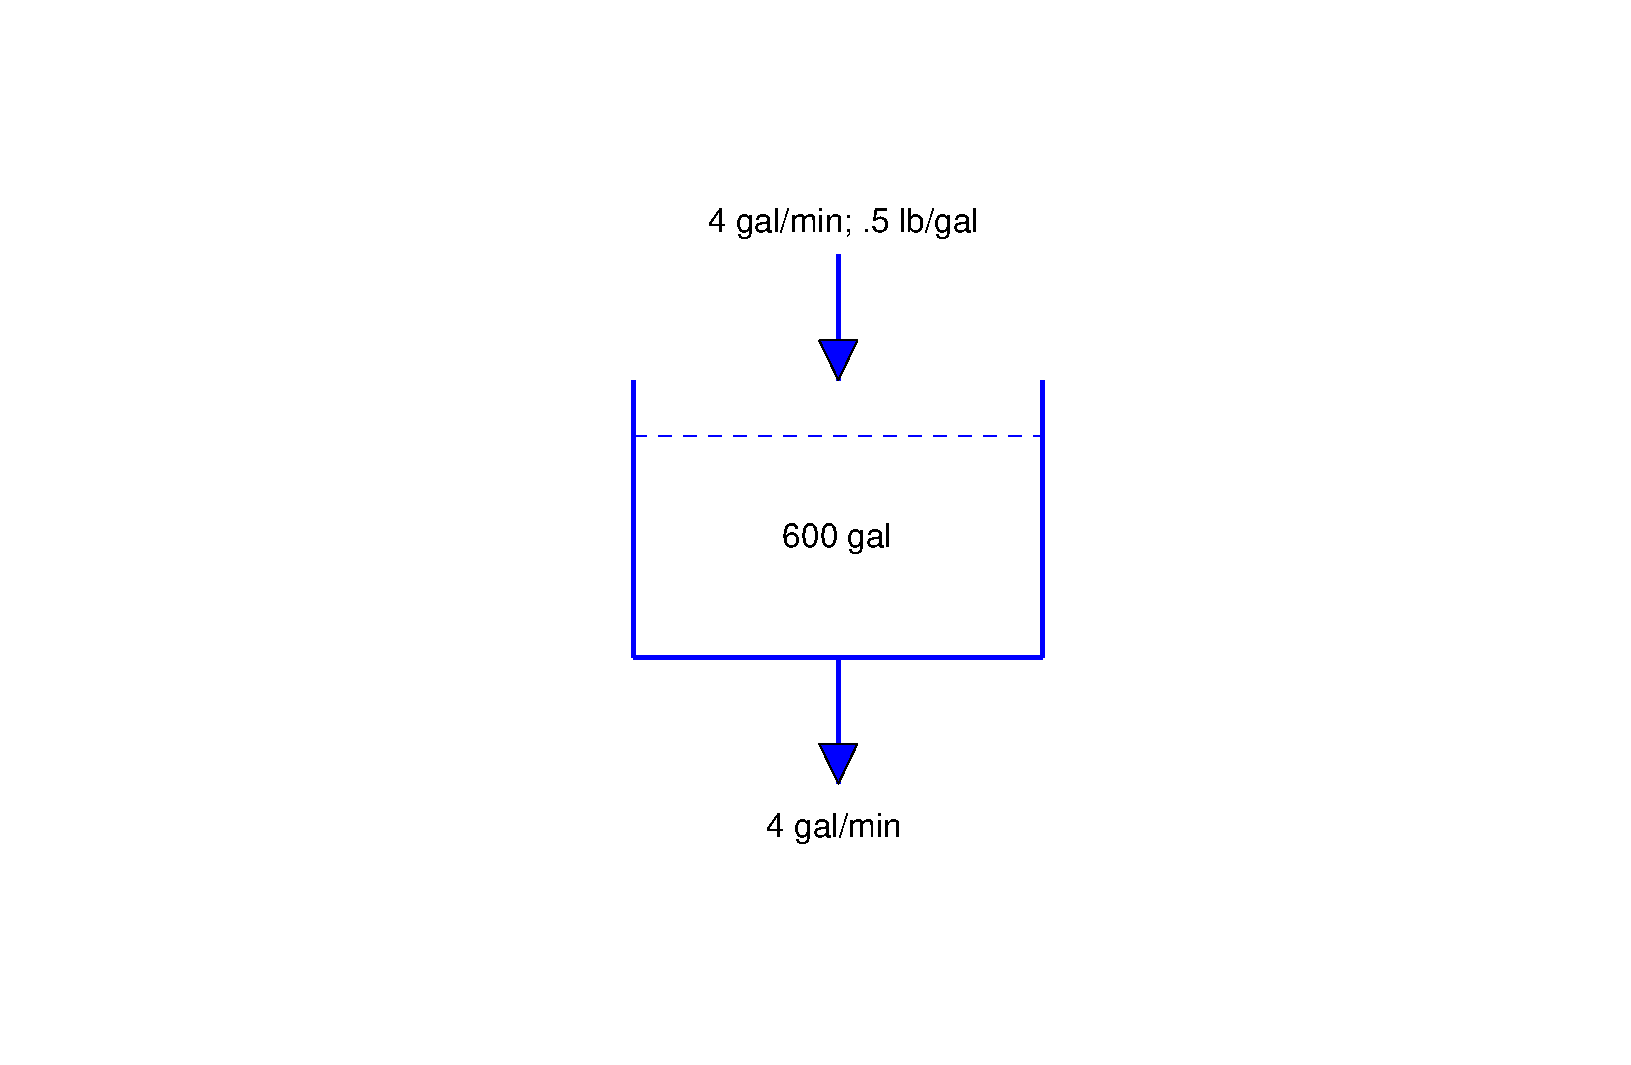
\includegraphics[bb=-78 148 689 643,width=5.67in,height=3.66in,keepaspectratio]{fig040203}
\color{blue}
  \caption{A mixing problem}
  \label{figure:4.2.3}
\end{figure}

\solutionpart{a} To find a differential equation for $Q$, we must use
the given information to derive an expression for $Q'$. But $Q'$
is the rate of change of the quantity of salt in the tank changes with
respect to time;
  thus, if {\color{blue}\it rate in\/} denotes the rate at which
salt enters
the tank and {\color{blue}\it rate out\/} denotes the rate by which it
leaves, then
\begin{equation} \label{eq:4.2.5}
Q' = \mbox{rate in}-\mbox{rate out}.
\end{equation}
The rate in is
$$
\left({1\over 2}\  \mbox{lb/gal}\right) \times (4\  \mbox{gal/min}) = 2\
\mbox{lb/min}.
$$
Determining the rate out requires a little more thought. We're
removing 4 gallons of the mixture per minute, and there are always 600
gallons in the tank; that is, we're removing $1/150$ of the mixture
per minute. Since the salt is evenly distributed in the mixture, we
are also removing $1/150$ of the salt per minute. Therefore, if there
are $Q(t)$ pounds of salt in the tank at time $t$, the rate out
at any time $t$ is $Q(t)/150$. Alternatively, we can arrive at this
conclusion by arguing that
$$
\begin{array}{lcl}
\mbox{rate out} & = & (\mbox{concentration})\times(\mbox{rate of
flow out})\\[6pt] \mbox{}&=&(\mbox{lb/gal})\times(\mbox{gal/min})\\[10pt]
&=&\dst{Q(t)\over600}\times
4=\dst{Q(t)\over150}.
\end{array}
$$
 We can now
write \eqref{eq:4.2.5} as
$$
Q' = 2-{Q\over 150}.
$$
This first order equation can be rewritten as
$$
Q'+{Q\over 150} = 2.
$$
Since $e^{-t/150}$ is a solution of the complementary equation, the
solutions of this equation are of the form  $Q=ue^{-t/150}$, where
$u'e^{-t/150}=2$, so $u'=2e^{t/150}$. Hence,
$$
u = 300e^{t/150}+c,
$$
 so
\begin{equation} \label{eq:4.2.6}
Q=ue^{-t/150}=300+ce^{-t/150}
\end{equation}
(Figure~\ref{figure:4.2.4}).
 Since $Q(0)=40$,  $c=-260$;  therefore,
$$
Q=300-260e^{-t/150}.
$$

\solutionpart{b} From \eqref{eq:4.2.6}, we see that that $\lim_{t \to
\infty}Q(t)=300$ for any value of  $Q(0)$. This is
intuitively reasonable, since the incoming solution contains 1/2
pound of salt per gallon and there are always 600 gallons of water in
the tank. \quad

\begin{example}\label{example:4.2.4} \rm
A 500-liter tank initially contains 10 g of salt dissolved in 200
liters of water. Starting at $t_0=0$, water that contains 1/4 g of salt
per liter is poured into the tank at the rate of 4 liters/min and the
mixture is drained from the tank at the rate of 2 liters/min
(Figure~\ref{figure:4.2.5}). Find a
differential equation for the quantity $Q(t)$ of salt in the tank at
time $t$ prior to the time when the tank overflows and find the
concentration $K(t)$ (g/liter ) of salt in the tank at any such time.
\end{example}

\begin{figure}[tbp]
  \centering
  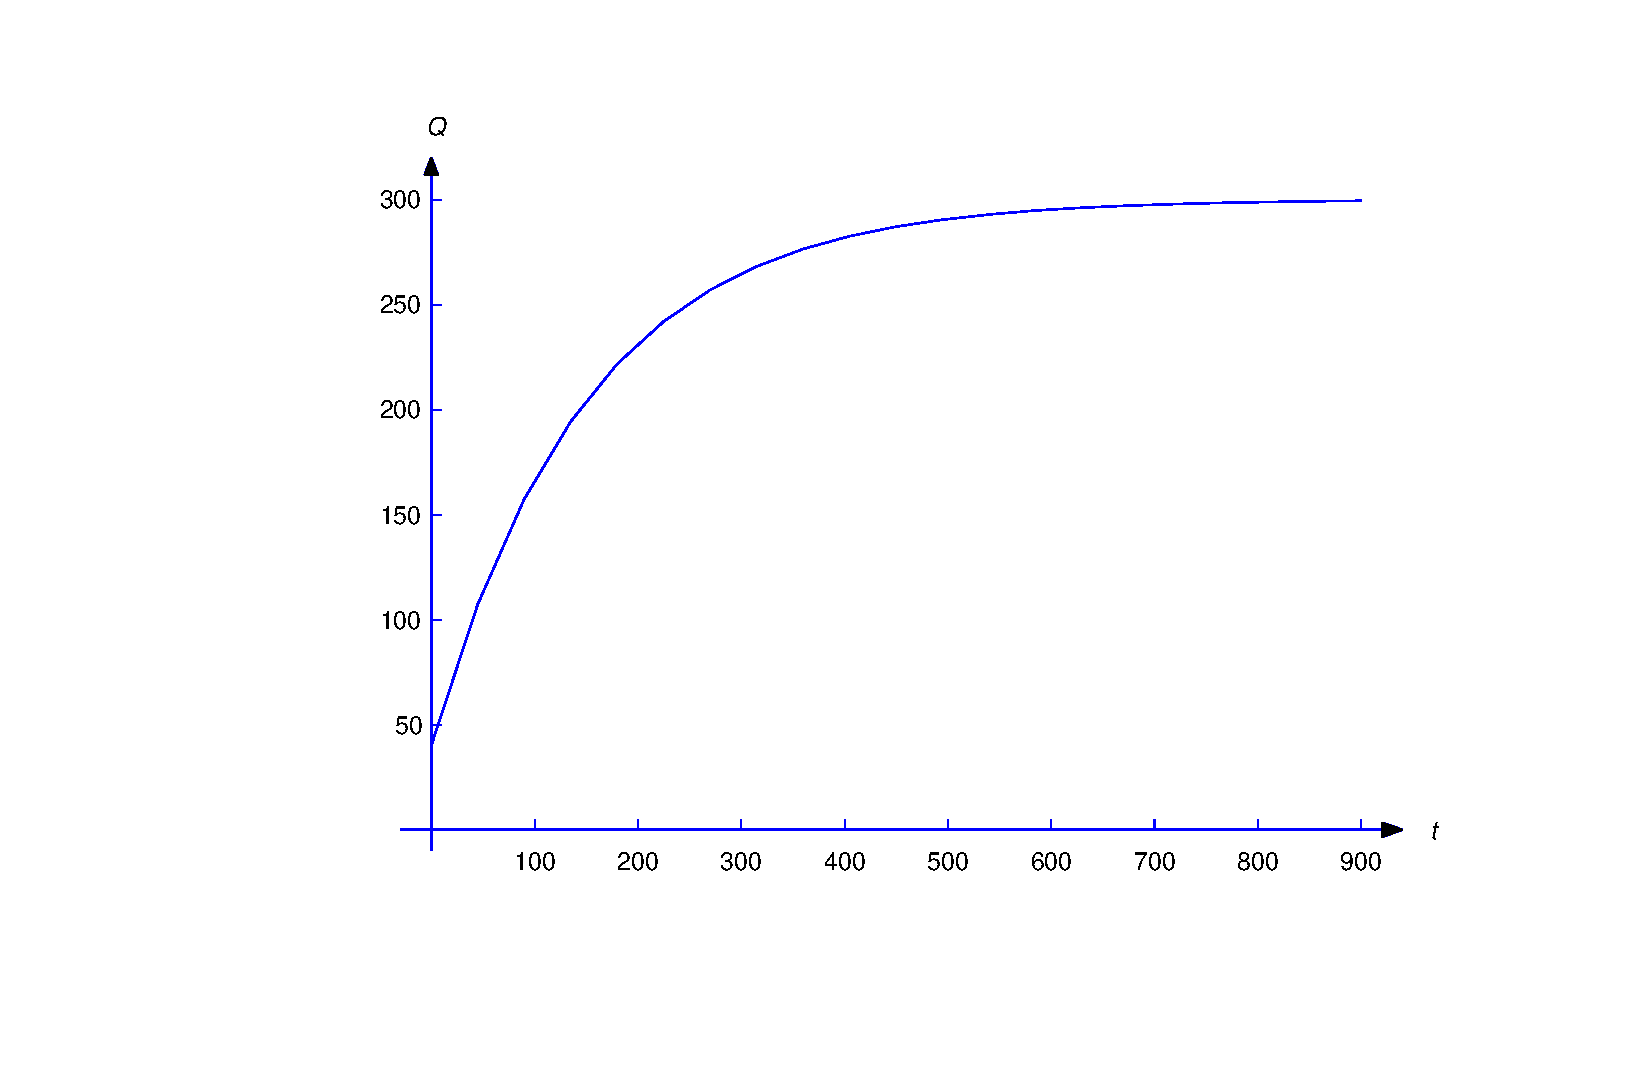
\includegraphics[bb=-78 148 689 643,width=5.67in,height=3.66in,keepaspectratio]{fig040204}
\color{blue}
  \caption{$Q=300-260e^{-t/150}$}
  \label{figure:4.2.4}
\end{figure}

\begin{figure}[tbp]
  \centering
  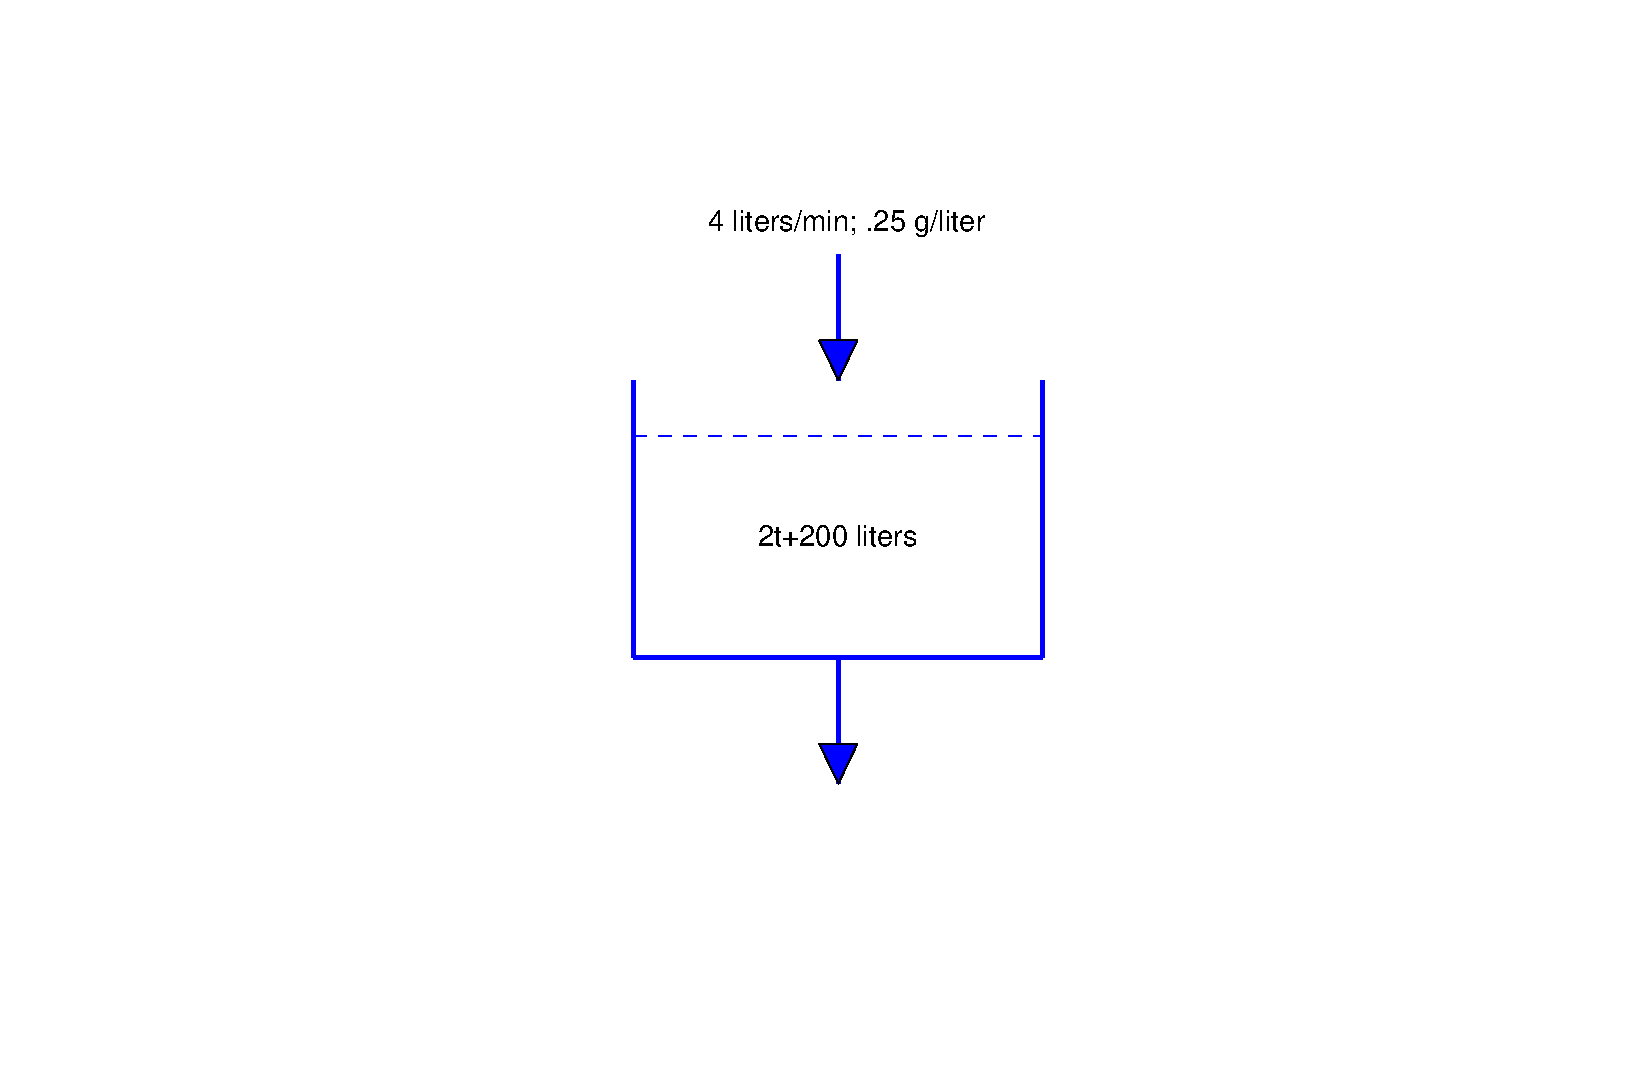
\includegraphics[bb=-78 148 689 643,width=5.67in,height=3.66in,keepaspectratio]{fig040205}
\color{blue}
  \caption{Another mixing problem}
  \label{figure:4.2.5}
\end{figure}

\solution  We first determine the
amount $W(t)$ of solution in the tank at any time $t$ prior to
overflow.  Since $W(0) = 200$ and we're adding 4 liters/min while
 removing only 2 liters/min, there's a net gain
of 2 liters/min in the tank;  therefore,
$$
W(t) = 2t+200.
$$
 Since $W(150)=500$ liters (capacity of the
tank), this formula is valid for $0 \le t \le 150$.

Now let $Q(t)$ be the number of grams of salt in the tank
at time $t$, where  $0 \le t \le 150$.  As in Example~\ref{example:4.2.3},
\begin{equation} \label{eq:4.2.7}
Q' = \mbox{rate in}-\mbox{rate out}.
\end{equation}
 The rate in is
\begin{equation} \label{eq:4.2.8}
\left({1\over 4}\  \mbox{g/liter}\,\right) \times (4\
\mbox{liters/min}\,) = 1\  \mbox{g/min}.
\end{equation}
 To determine the rate out, we observe that since
the mixture is being removed from the tank at the constant
rate of 2 liters/min and there are $2t+200$
liters in the tank at time $t$, the fraction of the mixture
being removed per minute at time $t$ is
$$
{2\over 2t+200} = {1\over t+100}.
$$
We're removing this same fraction of the salt per
minute.  Therefore, since there are $Q(t)$ grams of salt in
the tank at time $t$,
\begin{equation} \label{eq:4.2.9}
\mbox{rate out} = {Q(t)\over t+100}.
\end{equation}
Alternatively, we can arrive at this conclusion by arguing that
$$
\begin{array}{lcl}
\mbox{rate out} & = & (\mbox{concentration})\times(\mbox{rate of
flow out})
=(\mbox{g/liter})\times(\mbox{liters/min})\\[10pt]
&=&\dst{Q(t)\over2t+200}\times
2=\dst{Q(t)\over t+100}.
\end{array}
$$
 Substituting \eqref{eq:4.2.8} and \eqref{eq:4.2.9} into \eqref{eq:4.2.7}
yields
\begin{equation} \label{eq:4.2.10}
Q'=1-{Q\over t+100},\quad\text{ \rm so }\quad
Q'+{1\over t+100} Q=1.
\end{equation}
By separation of variables, $1/(t+100)$ is a solution of the
complementary equation, so the solutions of \eqref{eq:4.2.10}
are of the form
$$
Q={u\over t+100},\mbox{\quad where \quad}{u'\over t+100}=1,\mbox{\quad
so \quad} u'=t+100.
$$
Hence,
\begin{equation} \label{eq:4.2.11}
u = {(t+100)^2\over 2}+c.
\end{equation}
Since $Q(0)=10$  and $u=(t+100)Q$, \eqref{eq:4.2.11} implies that
$$
(100)(10) = {(100)^2\over 2}+c,
$$
so
$$
c=100(10)-{(100)^2\over 2} =-4000
$$
and therefore
$$
u = {(t+100)^2\over 2} -4000.
$$
 Hence,
 $$
Q = {u\over t+200}= {t+100\over 2}-{4000\over t+100}.
$$
Now let $K(t)$ be the concentration of salt at
time $t$.  Then
$$
K(t) = {1\over 4}-{2000\over(t+100)^2}
$$
(Figure~\ref{figure:4.2.6}).
          \begin{figure}[H]
  \centering
  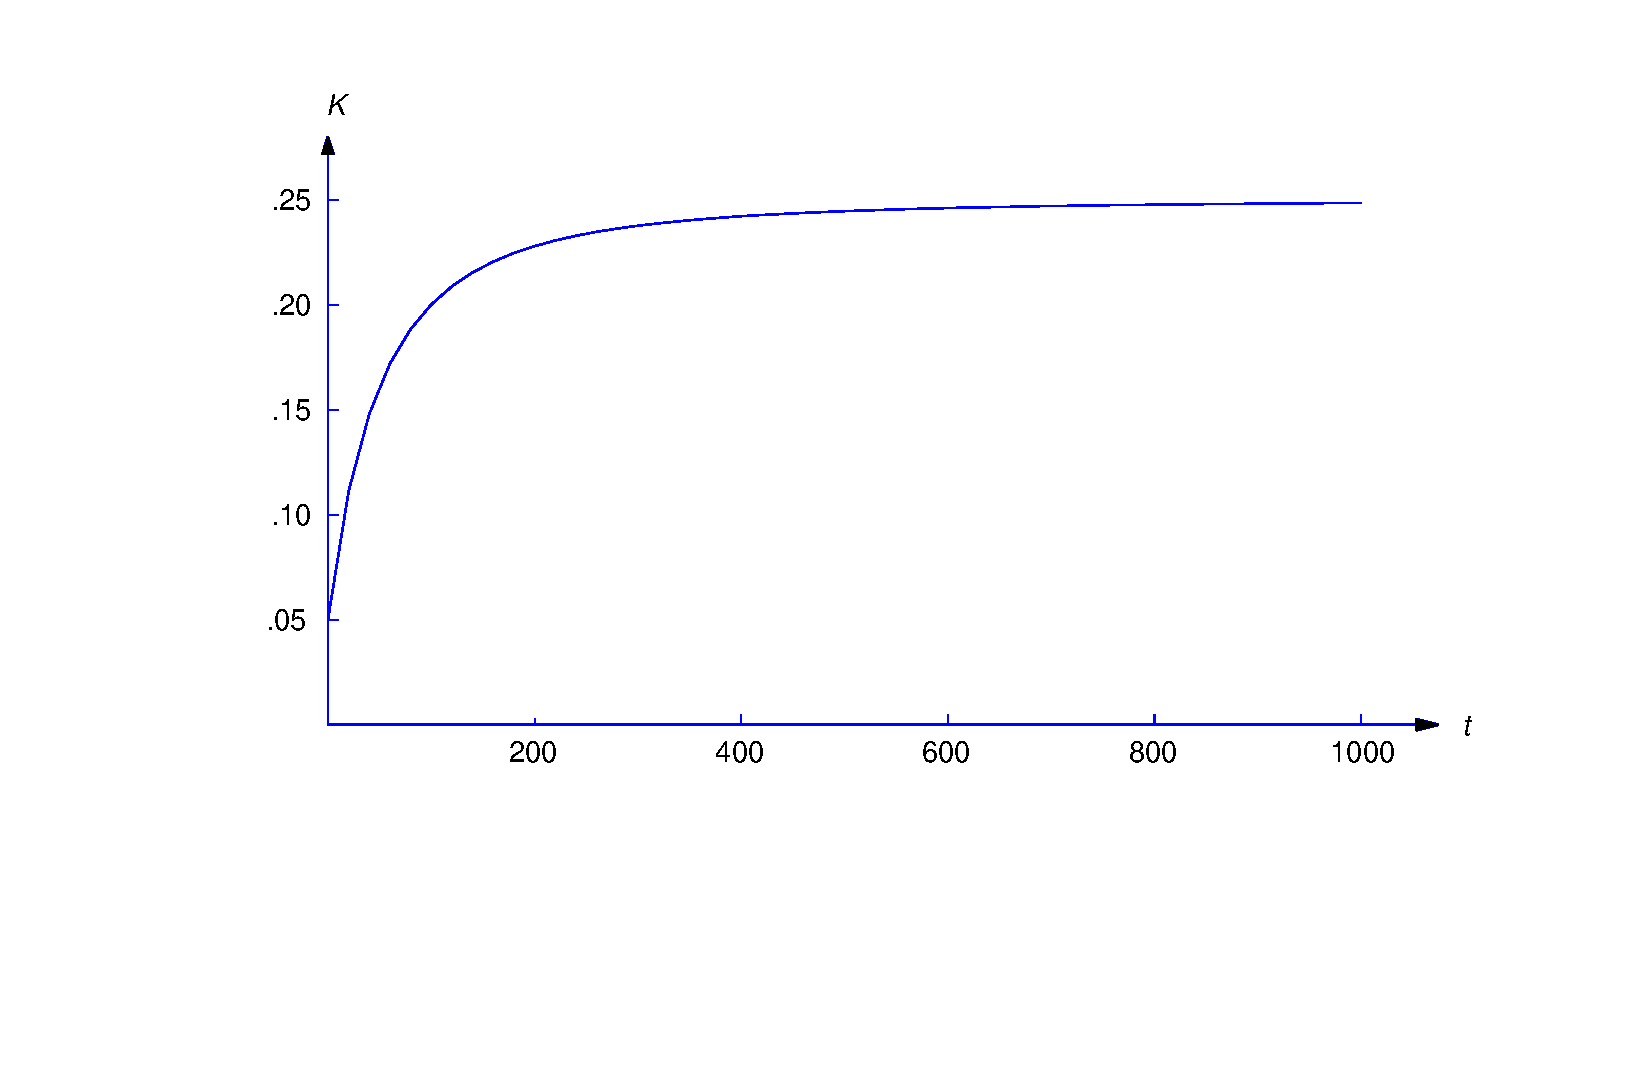
\includegraphics[bb=-78 148 689 643,width=5.67in,height=3.66in,keepaspectratio]{fig040206}
\color{blue}
  \caption{$K(t) = \dst{{1\over 4}-{2000\over(t+100)^2}}$}
  \label{figure:4.2.6}
\end{figure}

\newpage
\exercises

\begin{exerciselist}
\item\label{exer:4.2.1}
A thermometer is moved from a room where the temperature is
$70^\circ$F to a freezer where the temperature is $12^\circ
F$.  After 30 seconds the thermometer reads
$40^\circ$F.  What does it read after 2 minutes?

\item\label{exer:4.2.2}
A fluid initially at $100^\circ$C is placed outside on a
day when the temperature is $-10^\circ$C, and the
temperature of the fluid drops $20^\circ$C in one minute.
Find the temperature $T(t)$ of the fluid for $t > 0$.

\item\label{exer:4.2.3}
At 12:00 {\sc pm} a thermometer reading $10^\circ$F is placed in
a room where the temperature is $70^\circ$F.  It reads
$56^\circ$ when it's placed outside, where the temperature
is $5^\circ$F, at 12:03.  What does it read at 12:05 {\sc pm}?

\item\label{exer:4.2.4}
A thermometer initially reading $212^\circ$F is placed in a
room where the temperature is $70^\circ$F.  After 2
minutes the thermometer reads $125^\circ$F.

\begin{alist}
\item %(a)
What does the thermometer read after 4 minutes?

\item %(b)
When will the thermometer read $72^\circ$F?

\item %(c)
When will the thermometer read $69^\circ$F?
\end{alist}

\item\label{exer:4.2.5}
An object with initial temperature $150^\circ$C is placed
outside, where the temperature is $35^\circ$C.  Its
temperatures at 12:15 and 12:20 are $120^\circ$C and
$90^\circ$C, respectively.

\begin{alist}
\item %(a)
At what time was the object placed outside?

\item %(b)
When will its temperature be $40^\circ$C?
\end{alist}

\item\label{exer:4.2.6}
An object is placed in a room where the temperature is
$20^\circ$C.  The temperature of the object drops by
$5^\circ$C in 4 minutes and by $7^\circ$C in 8 minutes.
What was the temperature of the object when it was initially
placed in the room?

\item\label{exer:4.2.7}
A cup of boiling water is placed outside at 1:00 {\sc pm}.  One
minute later the temperature of the water is $152^\circ$F.
After another minute its temperature is $112^\circ$F.  What
is the outside temperature?

\item\label{exer:4.2.8}
A tank initially contains 40 gallons of pure water.  A
solution with 1 gram of salt per gallon of water is added
to the tank at 3 gal/min, and the  resulting
solution dranes out at the same rate.  Find the quantity $Q(t)$
of salt in the tank at time $t > 0$.

\item\label{exer:4.2.9}
A tank initially contains a solution of 10 pounds of salt in
60 gallons of water.  Water with 1/2 pound of salt per
gallon is added to the tank at 6 gal/min, and the
 resulting solution leaves at the same rate.
Find the quantity $Q(t)$ of salt in the tank at time
$t > 0$.

\item\label{exer:4.2.10}
A  tank initially contains 100 liters of a salt solution
with a concentration of .1 g/liter.  A solution with a
salt concentration of .3 g/liter is added to the tank at
5 liters/min, and the resulting mixture is
drained out at the same rate.  Find the concentration $K(t)$
of salt in the tank as a function of $t$.

\item\label{exer:4.2.11}
A 200 gallon tank initially contains 100 gallons of water
with 20 pounds of salt.  A salt solution with 1/4 pound of
salt per gallon is added to the tank at 4 gal/min, and the
resulting  mixture is drained out at 2 gal/min.
Find the quantity of salt in the tank as it's about to
overflow.

\item\label{exer:4.2.12}
Suppose  water is added to a tank at 10 gal/min, but leaks
out at the rate of 1/5 gal/min for each gallon in the tank.
What is the smallest capacity the tank can have if the
process is to continue indefinitely?

\item\label{exer:4.2.13}
A chemical reaction in a laboratory with volume $V$ (in ft$^3$)
produces $q_1$ ft$^3$/min of a noxious gas as a byproduct. The gas is
dangerous at concentrations greater than $\overline c$,
 but harmless at
concentrations $\le \overline c$. Intake fans at one end of the
laboratory pull in fresh air at the rate of $q_2$ ft$^3$/min and
exhaust fans at the other end exhaust the mixture of gas and air from
the
laboratory at the same rate. Assuming that the gas is always uniformly
distributed in the room and its initial concentration $c_0$ is at a
safe level, find the smallest value of $q_2$ required to maintain safe
conditions in the laboratory for all time.

\item\label{exer:4.2.14}
A 1200-gallon tank initially contains 40 pounds of salt
dissolved in 600 gallons of water.  Starting at $t_0=0$,
water that contains 1/2 pound of salt per gallon is added to
the tank at the rate of 6 gal/min and the
resulting mixture  is drained from the tank at 4 gal/min.  Find the
quantity $Q(t)$ of salt in the tank at any time $t > 0$
prior to overflow.

\item\label{exer:4.2.15}
Tank $T_1$  initially contain 50 gallons of pure water. Starting at
$t_0=0$,  water that contains 1 pound of salt per gallon is poured into
$T_1$ at  the rate of  2 gal/min.
The  mixture is drained from
$T_1$ at the same rate into a second tank $T_2$, which initially
contains  50 gallons of pure water.  Also starting at
$t_0=0$, a mixture from another source that contains 2  pounds of salt
per gallon is poured
into $T_2$  at the rate of 2 gal/min.  The  mixture is drained
from $T_2$ at the rate of 4 gal/min.

\begin{alist}
\item % (a)
 Find a differential
equation for the quantity $Q(t)$ of salt in  tank $T_2$ at time $t > 0$.
\item % (b)
Solve the equation derived  in \part{a} to determine $Q(t)$.
\item % (c)
 Find $\lim_{t\to\infty}Q(t)$.
\end{alist}

\item\label{exer:4.2.16}
Suppose an object  with initial temperature $T_0$
is placed in a sealed container, which is in turn placed in a medium with
temperature $T_m$. Let the initial
temperature of the container be $S_0$. Assume that the temperature of the
object does not affect the temperature of the container, which in turn does
not affect the temperature of the medium. (These assumptions  are
reasonable, for example, if the object is a cup of coffee, the container is
a house, and the medium is the atmosphere.)

\begin{alist}
\item % (a)
Assuming that the container and the medium have distinct temperature
decay constants $k$ and $k_m$ respectively, use Newton's law of
cooling to find the temperatures $S(t)$ and $T(t)$ of the container
and object at time $t$.

\item % (b)
Assuming that the container and the medium have the same temperature
decay constant $k$, use Newton's law of cooling to find the
temperatures $S(t)$ and $T(t)$ of the container and object at time
$t$.

\item % (c)
Find $\lim._{t\to\infty}S(t)$  and $\lim_{t\to\infty}T(t)$ .
\end{alist}

\item\label{exer:4.2.17}  %\exercisemolten
In  our previous examples and exercises concerning Newton's law of cooling
we assumed that
the temperature of the medium remains constant.  This model is adequate
if the heat lost or gained by the object is
insignificant compared to the heat required to cause an appreciable change
in the temperature of the medium. If this isn't  so,  we
must use a model that accounts for the heat exchanged between the object
and the medium. Let $T=T(t)$ and $T_m=T_m(t)$  be the temperatures of the
object and the medium, respectively, and let $T_0$  and $T_{m0}$ be
their
initial values.  Again, we assume that $T$  and $T_m$ are related by
Newton's law of cooling,
$$
T'=-k(T-T_m).
\eqno{\rm (A)}
$$
We also assume that the change in heat of the object as its
temperature changes from $T_0$ to $T$  is $a(T-T_0)$
and that the change in heat of the medium  as its
temperature changes from $T_{m0}$ to $T_m$  is $a_m(T_m-T_{m0})$,
where $a$
and $a_m$ are positive constants  depending  upon the masses and
thermal properties of the
object and medium, respectively.  If we assume that the total heat of
the system consisting of the object and the medium remains constant
(that is, energy is conserved), then
$$
a(T-T_0)+a_m(T_m-T_{m0})=0.
\eqno{\rm (B)}
$$

\begin{alist}
\item % (a)
Equation (A) involves  two unknown functions $T$ and $T_m$.
 Use (A) and (B) to derive a
differential equation involving only $T$.
\item % (b)
Find $T(t)$ and $T_m(t)$ for $t>0$.
\item % (c)
Find $\lim_{t\to\infty}T(t)$ and
 $\lim_{t\to\infty}T_m(t)$.
\end{alist}

\item\label{exer:4.2.18} Control mechanisms allow fluid to flow into a tank
at a rate proportional to the volume $V$ of fluid in the tank, and to
flow
out at a rate proportional to $V^2$. Suppose $V(0)=V_0$ and the
constants of proportionality are $a$ and $b$, respectively.
Find $V(t)$  for $t>0$ and find $\lim_{t\to\infty}V(t)$.

\item\label{exer:4.2.19}
Identical tanks $T_1$ and $T_2$ initially contain $W$ gallons each of
pure water. Starting at $t_0=0$, a salt solution with constant
concentration $c$ is pumped into $T_1$ at $r$ gal/min and drained from
$T_1$ into $T_2$ at the same rate. The resulting mixture in $T_2$ is
also drained at the same rate. Find the concentrations $c_1(t)$
and $c_2(t)$ in tanks $T_1$ and $T_2$ for $t>0$.

\item\label{exer:4.2.20}
An infinite sequence of identical tanks $T_1$, $T_2$, \dots, $T_n$, \dots,
initially contain $W$ gallons
each of pure water.  They are hooked together so that fluid drains
from $T_n$ into  $T_{n+1}\,(n=1,2,\cdots)$.
A salt solution is circulated through the tanks so that it enters and
leaves each tank at the constant rate of $r$ gal/min.
The solution has a concentration of
$c$  pounds of salt per
gallon when it enters $T_1$.

\begin{alist}
\item % (a)
Find the concentration $c_n(t)$
in tank $T_n$ for $t>0$.
\item % (b)
  Find $\lim_{t\to\infty}c_n(t)$ for each $n$.
\end{alist}

\item\label{exer:4.2.21}
Tanks $T_1$  and $T_2$ have capacities $W_1$ and $W_2$ liters,
respectively.
Initially they are both full of dye solutions with concentrations $c_{1}$
and $c_2$ grams per liter. Starting at $t_0=0$,  the solution from $T_1$
is pumped into $T_2$ at a rate of $r$  liters per minute,
and the solution from $T_2$
is pumped into $T_1$ at the same rate.

\begin{alist}
\item % (a)
Find the concentrations $c_1(t)$ and $c_2(t)$ of the dye in $T_1$
and $T_2$ for $t>0$.
\item % (b)
Find $\lim_{t\to\infty}c_1(t)$  and $\lim_{t\to\infty}c_2(t)$.
\end{alist}

\item\label{exer:4.2.22} \Lex
Consider the mixing problem of Example~\ref{example:4.2.3}, but without
the assumption that the mixture is stirred instantly so that the salt
is always uniformly distributed throughout the mixture. Assume instead
that the distribution approaches uniformity as $t\to\infty$.
In this case the differential equation for $Q$ is  of the form
$$
Q'+{a(t)\over150}Q=2
$$
where  $\lim_{t\to\infty}a(t)=1$.
\begin{alist}
\item % (a)
Assuming that
$Q(0)=Q_0$, can you guess the value of
$\lim_{t\to\infty}Q(t)$?.
\item % (b)
Use numerical methods to  confirm  your guess in the these cases:
$$
\mbox{\part{i}\;   }  a(t)=t/(1+t)  \mbox{\quad    \part{ii}\;  }
a(t)=1-e^{-t^2}  \mbox{\quad    \part{iii}\;  }
 a(t)=1-\sin(e^{-t}).
$$
\end{alist}

\item\label{exer:4.2.23} \Lex
Consider the mixing problem of Example~\ref{example:4.2.4} in a tank with
infinite capacity, but without the assumption that the mixture is
stirred instantly so that the salt is always uniformly distributed
throughout the mixture. Assume instead that the distribution
approaches uniformity as $t\to\infty$. In this case the differential
equation for $Q$ is of the form
$$
Q'+{a(t)\over t+100}Q=1
$$
where  $\lim_{t\to\infty}a(t)=1$.
\begin{alist}
\item % (a)
Let $K(t)$ be the concentration of salt at time $t$. Assuming that
$Q(0)=Q_0$, can you guess the value of $\lim_{t\to\infty}K(t)$?
\item % (b)
Use numerical methods to  confirm  your guess in the these cases:
$$
\mbox{\part{i}\;  }  a(t)=t/(1+t)\; \mbox{\;   \part{ii}\;   }
a(t)=1-e^{-t^2}  \mbox{\;   \part{iii}\;   }
 a(t)=1+\sin(e^{-t}).
$$
\end{alist}

\end{exerciselist}


\newsection{3}{Applications of First Order Equations} {Elementary Mechanics}
\currentpdfbookmark{Section 4.3 Elementary Mechanics}{section:4.3}
\vskip14pt
\renewcommand{\thissection}{\sectiontitle{\,
ELEMENTARY MECHANICS}}
\thissection

\boxit{Newton's Second Law of Motion}

\noindent
In this section we consider an object with constant mass $m$ moving
along a line under a force $F$. Let $y=y(t)$ be the displacement of
the object from a reference point on the line at time $t$, and let
$v=v(t)$ and $a=a(t)$ be the velocity and acceleration of the object
at time $t$. Thus, $v=y'$ and $a=v'=y''$, where the prime denotes
differentiation with respect to $t$. Newton's second law of motion
asserts that the force $F$ and the acceleration $a$ are related by the
equation
\begin{equation} \label{eq:4.3.1}
F=ma.
\end{equation}

\boxit{Units}

\noindent
In applications there are three main sets of units in use for length,
mass, force, and time: the cgs, mks, and British systems. All three
use the second as the unit of time. Table~1 shows the other units.
 Consistent with (\ref{eq:4.3.1}), the unit of
force in each system is defined to be the force required to impart an
acceleration of (one unit of length)$/s^2$ to one unit of
mass.

\bigskip
\begin{center}
\begin{tabular}{|c|c|c|c|}
\hline
& {\bf Length}&{\bf Force}& {\bf Mass}\\\hline
  cgs & centimeter (cm) & dyne (d) & gram (g)\\\hline
 mks & meter (m) & newton (N) & kilogram (kg) \\\hline
British & foot (ft) & pound (lb) & slug (sl)\\\hline
\end{tabular}

\medskip
Table 1.
\end{center}

If we assume that Earth is a perfect sphere with constant mass
density,  Newton's law of gravitation (discussed later in this
section) asserts that the force exerted on an object by Earth's
gravitational field is proportional to the mass of the object and
inversely proportional to the square of its  distance from the
center of Earth. However, if the object remains sufficiently close to
Earth's surface, we may assume that the gravitational force is
constant and equal to its value at the surface. The magnitude of this
force is $mg$, where $g$ is called the {\color{blue}\it acceleration due to
gravity}. (To be completely accurate, $g$ should be called the {\color{blue}\it
magnitude of the acceleration due to gravity at Earth's surface}.)\
This quantity has been determined experimentally. Approximate
values of $g$  are
$$\begin{array}{rl}
g &=980\ \mbox{cm/s}^2 \hskip40pt \mbox{(cgs)}   \\
g &=9.8\ \mbox{m/s}^2 \hskip48pt \mbox{(mks)}   \\
g &=32\ \mbox{ft/s}^2 \hskip52pt \mbox{(British)}.
\end{array}$$

In general, the force $F$ in (\ref{eq:4.3.1}) may depend upon $t$, $y$, and
$y'$. Since $a=y''$,  (\ref{eq:4.3.1}) can be written in the
form
\begin{equation} \label{eq:4.3.2}
my''=F(t,y,y'),
\end{equation}
which is a second order equation. We'll consider this equation with
restrictions on $F$ later;     however, since Chapter~2
dealt only with first order equations, we consider here only problems in
which (\ref{eq:4.3.2}) can be recast as a first order equation. This is
possible if $F$ does not depend on $y$, so (\ref{eq:4.3.2}) is of the form
$$
my''=F(t,y').
$$
 Letting $v=y'$ and $v'=y''$ yields a first order
equation for $v$:
\begin{equation} \label{eq:4.3.3}
mv'=F(t,v).
\end{equation}
Solving this equation yields $v$ as a function of $t$. If we know
$y(t_0)$ for some time $t_0$, we can  integrate $v$ to obtain $y$
as a function of $t$.

Equations of the form (\ref{eq:4.3.3}) occur in problems involving motion
through a resisting medium.

\boxit{Motion Through a Resisting Medium Under Constant
Gravitational Force}

\noindent
Now we consider an object moving vertically in some medium. We assume
that the only forces acting on the object are gravity and resistance
from the medium. We also assume that the motion takes place close to
Earth's surface and take the upward direction to be positive, so
 the gravitational force can be assumed to have the constant value
 $-mg$. We'll see that, under reasonable assumptions on the
resisting force, the velocity approaches a limit as $t\to\infty$.
We call this limit the {\color{blue}\it terminal velocity\/}.

\begin{example}\label{example:4.3.1} \rm
An object with mass $m$ moves under constant gravitational force
through a medium that exerts a resistance with magnitude proportional
to the speed of the object. (Recall that the speed of an object is
$|v|$, the absolute value of its velocity $v$.) Find the velocity of
the object as a function of $t$, and find the terminal velocity.
Assume  that the initial velocity is $v_0$.
 \end{example}

\solution
The total force acting on the object is
\begin{equation} \label{eq:4.3.4}
F=-mg+F_1,
\end{equation}
where $-mg$ is  the force due to  gravity and $F_1$ is the
resisting force of the medium, which has magnitude $k|v|$, where $k$ is a
positive constant. If the
object is moving downward ($v\le 0$),  the resisting force is
upward (Figure~\ref{figure:4.3.1}\part{a}), so
$$
F_1=k|v|=k(-v)=-kv.
$$
On the other hand, if the object is moving upward ($v\ge 0$),
the resisting force is downward (Figure~\ref{figure:4.3.1}\part{b}), so
$$
F_1=-k|v|=-kv.
$$
Thus, (\ref{eq:4.3.4}) can be written as
\begin{equation} \label{eq:4.3.5}
F=-mg-kv,
\end{equation}
regardless of the sign of the velocity.

\begin{figure}[tbp]
  \centering
  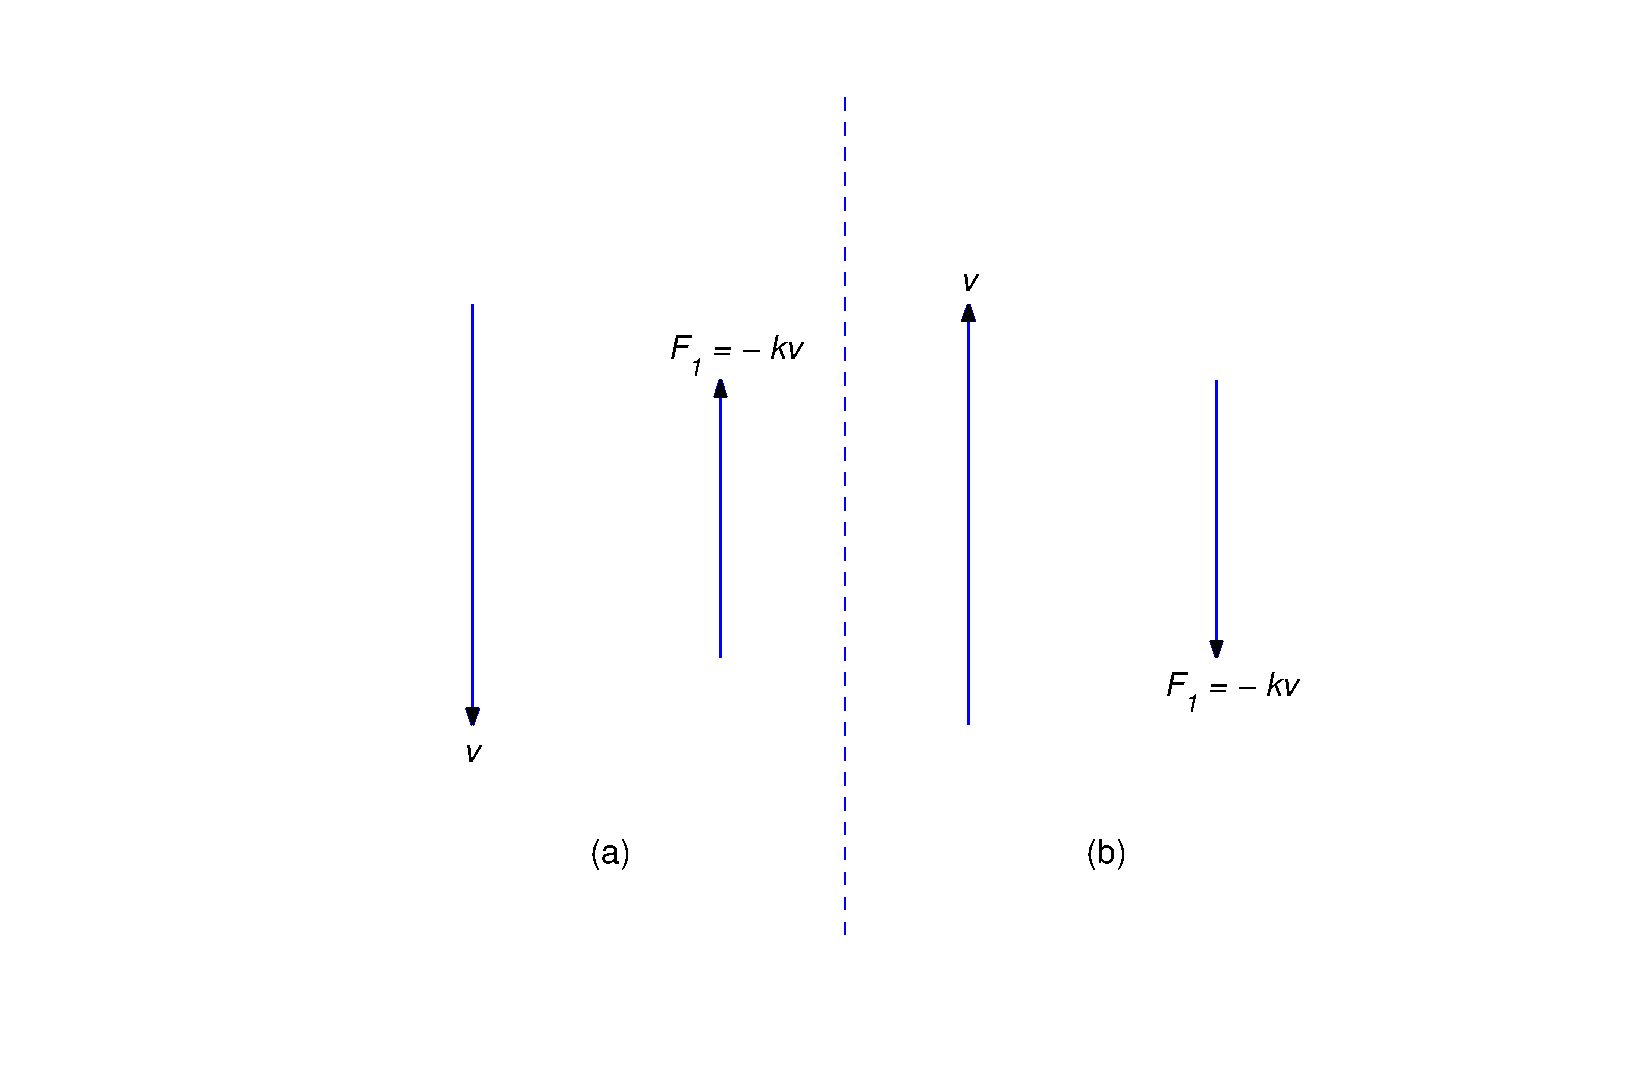
\includegraphics[bb=-78 148 689 643,width=5.67in,height=3.66in,keepaspectratio]{fig040301}
\color{blue}
  \caption{Resistive forces}
  \label{figure:4.3.1}
\end{figure}

From Newton's second law of motion,
$$
F=ma=mv',
$$
 so (\ref{eq:4.3.5}) yields
$$
mv'=-mg-kv,
$$
 or
\begin{equation} \label{eq:4.3.6}
v'+{k\over m}v=-g.
\end{equation}
Since $e^{-kt/m}$ is a solution of the  complementary
equation, the solutions of (\ref{eq:4.3.6}) are of the form
$v=ue^{-kt/m}$, where $u'e^{-kt/m}=-g$, so $u'=-ge^{kt/m}$.
Hence,
$$
u=-{mg\over k} e^{kt/m}+c,
$$
so
\begin{equation} \label{eq:4.3.7}
v=ue^{-kt/m}=-{mg\over k}+ce^{-kt/m}.
\end{equation}
Since
 $v(0)=v_0$,
$$
v_0=-{mg\over k}+c,
$$
 so
$$
c=v_0+{mg\over k}
$$
 and (\ref{eq:4.3.7}) becomes
$$
v=-{mg\over k}+\left(v_0+{mg\over k}\right) e^{-kt/m}.
$$
Letting $t\to\infty$ here shows that the terminal velocity is
$$
\lim_{t\to\infty} v(t)=-{mg\over k},
$$
which  is independent of the
initial velocity $v_0$ (Figure~\ref{figure:4.3.2}).

\begin{figure}[tbp]
  \centering
  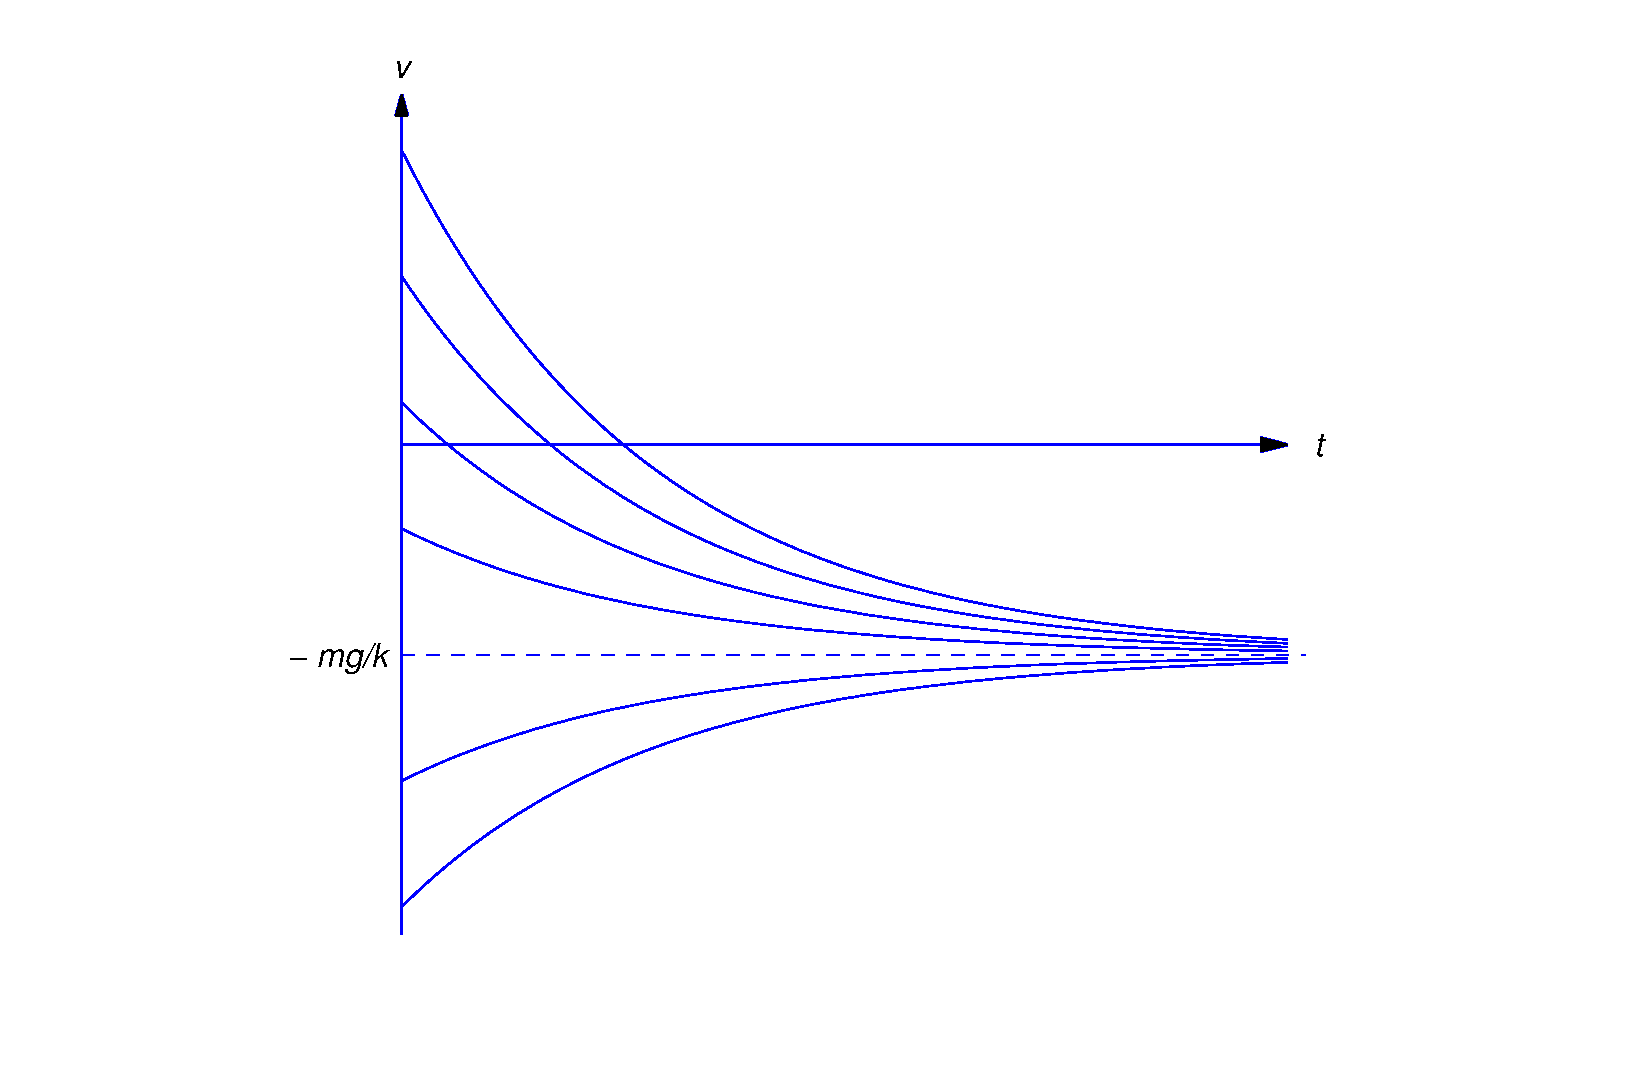
\includegraphics[bb=-78 148 689 643,width=5.67in,height=3.66in,keepaspectratio]{fig040302}
\color{blue}
  \caption{Solutions of $mv'=-mg-kv$}
  \label{figure:4.3.2}
\end{figure}

\begin{example}\label{example:4.3.2} \rm
A 960-lb object is given an initial upward velocity of 60 ft/s near
the surface of Earth. The atmosphere resists the motion with a force
of 3 lb for each ft/s of speed. Assuming that the only other force
acting on the object is constant gravity, find its velocity $v$ as a
function of $t$, and find its  terminal velocity.
\end{example}

\solution
Since $mg=960$ and $g=32$,   $m=960/32=30$.  The atmospheric
resistance is $-3v$  lb if $v$ is expressed in feet
per second.  Therefore
$$
30v'=-960-3v,
$$
which we rewrite as
$$
v'+{1\over 10}v=-32.
$$
Since $e^{-t/10}$ is a solution of the complementary equation, the
solutions of this equation are of the form $v=ue^{-t/10}$, where
$u'e^{-t/10}=-32$, so $u'=-32e^{t/10}$. Hence,
$$
u=-320 e^{t/10}+c,
$$
so
\begin{equation} \label{eq:4.3.8}
v=ue^{-t/10}=-320+ce^{-t/10}.
\end{equation}
The initial velocity is 60 ft/s in the upward (positive) direction;
hence, $v_0=60$. Substituting $t=0$ and $v=60$ in (\ref{eq:4.3.8})
yields
$$
60=-320+c,
$$
 so $c=380$, and (\ref{eq:4.3.8}) becomes
$$
v=-320+380e^{-t/10}\ \mbox{ft/s}
$$
The terminal velocity is
$$
\lim_{t\to\infty}v(t)=-320\mbox{ ft/s.}
$$

\begin{example}\label{example:4.3.3} \rm
A 10 kg mass is given an initial velocity $v_0\le0$
 near Earth's surface. The only forces acting on it are
gravity and atmospheric resistance proportional to the square of the
speed. Assuming that the resistance is 8 N if the speed is 2 m/s,
find the velocity of the object as a function of $t$, and
find the terminal velocity.
\end{example}

\solution Since the object is falling, the resistance is in the upward
(positive) direction. Hence,
\begin{equation} \label{eq:4.3.9}
mv'=-mg+kv^2,
\end{equation}
where $k$ is a constant. Since the magnitude of the resistance is 8 N
when $v=2$ m/s,
$$
k(2^2)=8,
$$
 so $k=2\  \mbox{N-s}^2/\mbox{m}^2$.  Since
$m=10$ and $g=9.8$, (\ref{eq:4.3.9}) becomes
\begin{equation} \label{eq:4.3.10}
10v'=-98+2v^2=2(v^2-49).
\end{equation}
If $v_0=-7$, then $v\equiv-7$ for all $t\ge0$. If $v_0\ne-7$,
we separate  variables to obtain
\begin{equation} \label{eq:4.3.11}
{1\over v^2-49}v'={1\over5},
\end{equation}
which is convenient for the required partial fraction expansion
\begin{equation} \label{eq:4.3.12}
\frac{1}{v^2-49} =\frac{1}{(v-7)(v+7)}
={1\over 14}\left[{1\over v-7}
-{1\over v+7}\right].
\end{equation}
 Substituting (\ref{eq:4.3.12})  into (\ref{eq:4.3.11}) yields
$$
{1\over14}\left[{1\over v-7}-{1\over v+7}\right]v'={1\over5},
$$
 so
$$
\left[{1\over v-7}-{1\over v+7}\right]v'={14\over5}.
$$
Integrating this yields
$$
\ln |v-7|-\ln|v+7|=14t/5+k.
$$
Therefore
$$
\left|{v-7\over v+7}\right|=e^ke^{14t/5}.
$$
Since  Theorem~\ref{thmtype:2.3.1}  implies  that  $(v-7)/(v+7)$   can't
change sign (why?), we can rewrite the last equation as
 \begin{equation} \label{eq:4.3.13}
 {v-7\over v+7}=ce^{14t/5},
\end{equation}
which is an implicit solution of (\ref{eq:4.3.10}).
Solving this for $v$ yields
\begin{equation} \label{eq:4.3.14}
v=-7{c+e^{-14t/5}\over c-e^{-14t/5}}.
\end{equation}
 Since $v(0)=v_0$, it
 (\ref{eq:4.3.13}) implies that
$$
c={v_0-7\over v_0+7}.
$$
 Substituting this into (\ref{eq:4.3.14}) and simplifying yields
$$
v=-7{v_0(1+e^{-14t/5})-7(1-e^{-14t/5})\over
v_0(1-e^{-14t/5})-7(1+e^{-14t/5}}.
$$
Since $v_0\le0$, $v$ is defined and negative for all
$t>0$. The terminal velocity is
$$
\lim_{t\to\infty} v(t)=-7\  \mbox{m/s},
$$
independent of $v_0$. More generally, it
can be shown (Exercise~\ref{exer:4.3.11}) that if $v$ is any solution
of (\ref{eq:4.3.9}) such that $v_0\le0$ then
$$
\lim_{t\to\infty}v(t)=-\sqrt{mg\over k}
$$
(Figure~\ref{figure:4.3.3}).

      \begin{figure}[tbp]
  \centering
  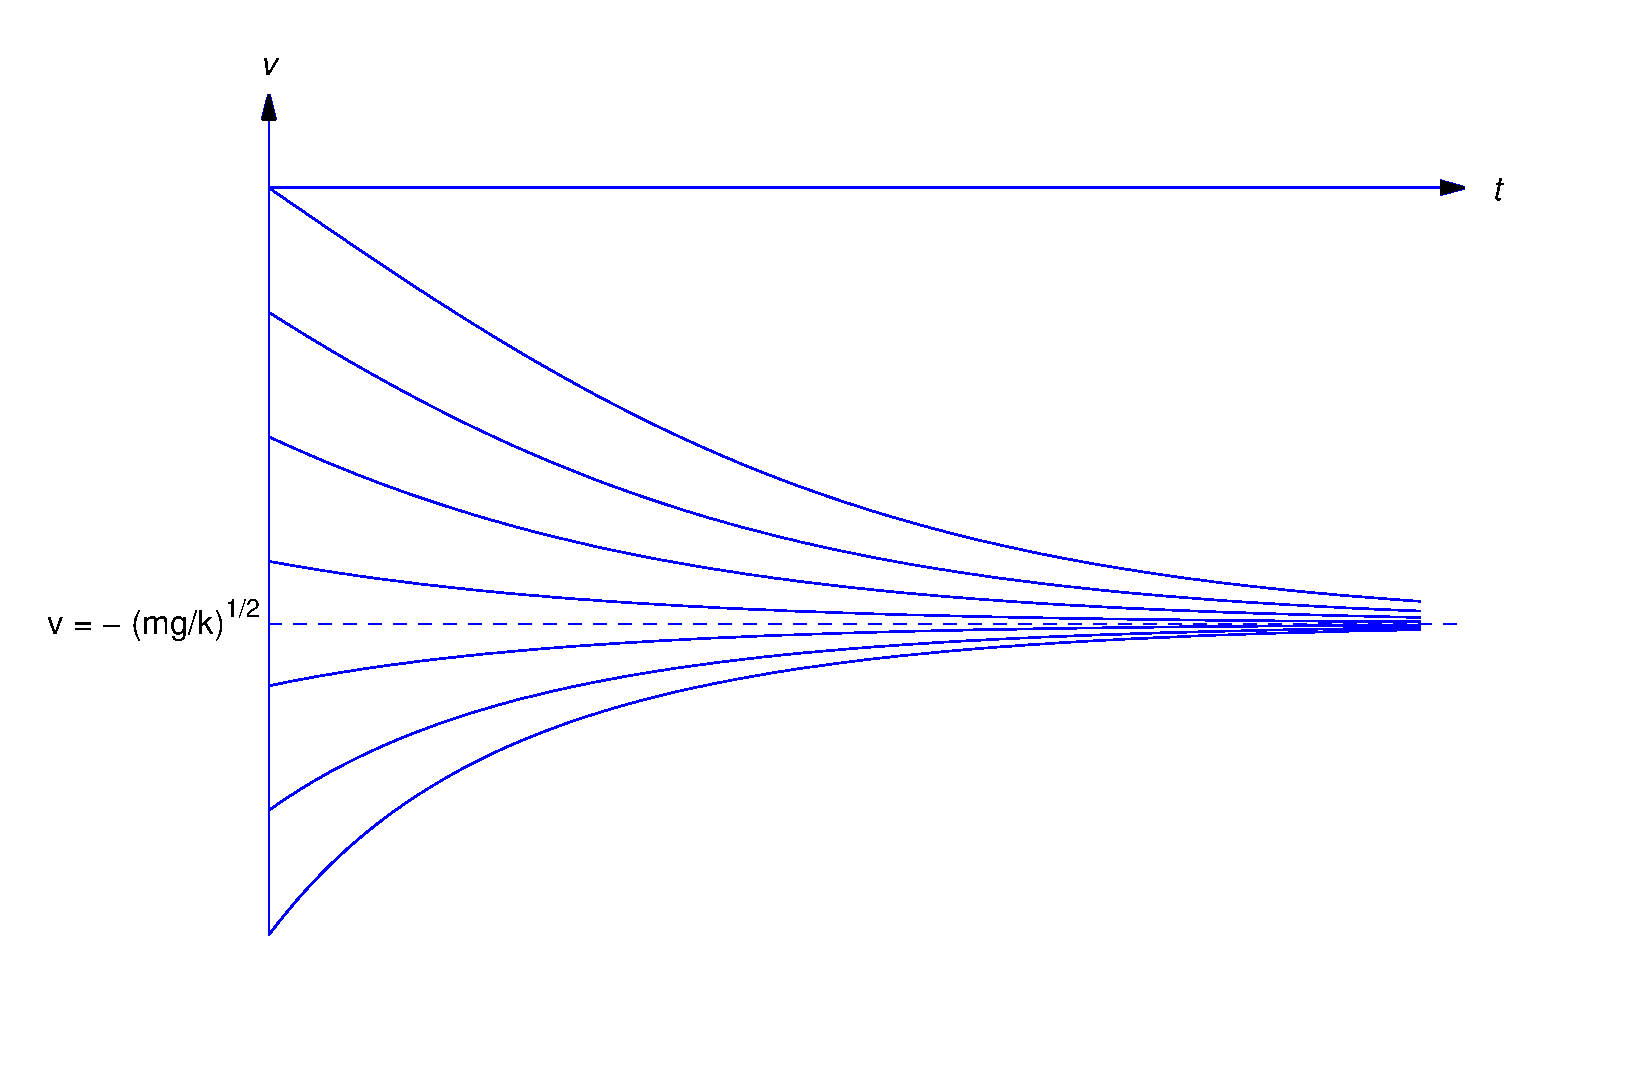
\includegraphics[bb=-78 148 689 643,width=5.67in,height=3.66in,keepaspectratio]{fig040303}
\color{blue}
  \caption{Solutions of $mv'=-mg+kv^2,\ v(0)=v_0\le0$}
  \label{figure:4.3.3}
\end{figure}

\begin{example}\label{example:4.3.4} \rm
A 10-kg mass is launched vertically upward from Earth's surface with
an initial velocity of $v_0$ m/s. The only forces acting on the mass
are gravity and atmospheric resistance proportional to the square of
the speed. Assuming that the atmospheric resistance is 8 N if the
speed is 2 m/s, find the time $T$ required for the mass to reach
maximum altitude.
\end{example}

\solution  The mass will
climb while $v>0 $ and reach its maximum altitude when $v=0$.
Therefore $v>0$ for $0\le t<T$ and $v(T)=0$. Although the mass of
the object and our assumptions concerning the forces acting on it are
the same as those in Example 3,  (\ref{eq:4.3.10}) does
not apply here, since the resisting force is negative if $v>0$;
therefore, we replace (\ref{eq:4.3.10}) by
\begin{equation} \label{eq:4.3.15}
10v'=-98-2v^2.
\end{equation}

Separating variables  yields
$$
{5\over v^2+49}v'=-1,
$$
 and integrating this yields
$$
{5\over7}\tan^{-1}{v\over7}=-t+c.
$$
 (Recall that $\tan^{-1}u$ is the number $\theta$
such that $-\pi/2 < \theta < \pi/2$ and $\tan \theta=u$.)
 Since $v(0)=v_0$,
$$
c={5\over7}\tan^{-1}{v_0\over7},
$$
so $v$ is defined implicitly by
\begin{equation} \label{eq:4.3.16}
{5\over7} \tan^{-1}{v\over7}=-t+{5\over7}
\tan^{-1}{v_0\over7}, \quad 0\le t\le T.
\end{equation}
Solving this for $v$ yields
\begin{equation} \label{eq:4.3.17}
v=7\tan\left(-{7t\over5}+\tan^{-1}{v_0\over7}\right).
\end{equation}
Using the identity
$$
\tan(A-B)={\tan A-\tan B\over1+\tan A\tan B}
$$
with $A=\tan^{-1}(v_0/7)$ and $B=7t/5$, and noting that
$\tan(\tan^{-1}\theta)=\theta$,
we can simplify (\ref{eq:4.3.17}) to
$$
v=7{v_0-7\tan(7t/5)\over7+v_0\tan(7t/5)}.
$$

 Since $v(T)=0$ and $\tan^{-1}(0)=0$, (\ref{eq:4.3.16}) implies that
$$
-T+{5\over7} \tan^{-1}{v_0\over7}=0.
$$
Therefore
$$
T={5\over7} \tan^{-1}{v_0\over7}.
$$
Since $\tan^{-1}(v_0/7)<\pi/2$ for all $v_0$,
the  time required for the mass to reach its maximum
altitude is less than
$$
{5\pi\over 14} \approx 1.122\  \mbox{s}
$$
regardless of the initial velocity.  Figure~\ref{figure:4.3.4}
shows graphs of $v$ over $[0,T]$ for various values of $v_0$.

\begin{figure}[tbp]
  \centering
  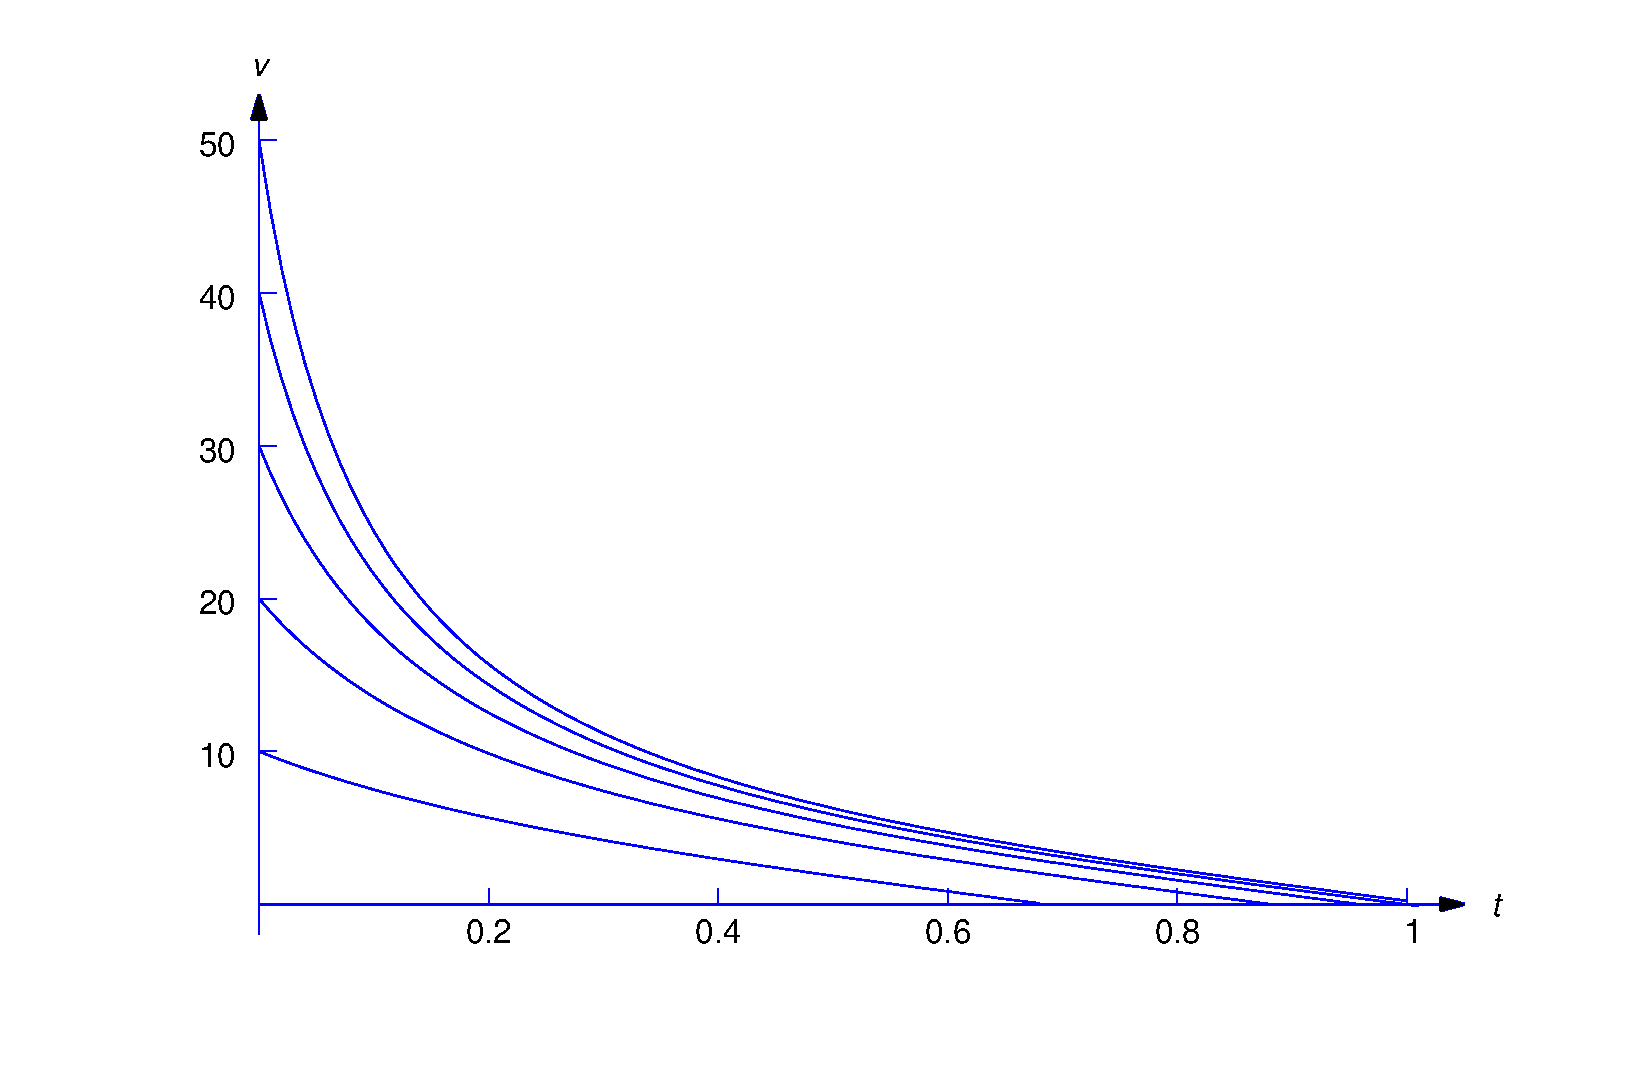
\includegraphics[bb=-78 148 689 643,width=5.67in,height=3.66in,keepaspectratio]{fig040304}
\color{blue}
\caption{Solutions of (\ref{eq:4.3.15}) for various
$v_0>0$}
  \label{figure:4.3.4}
\end{figure}

\newpage

\boxit{Escape Velocity}

\noindent
Suppose a space vehicle is launched vertically and its fuel is
exhausted when the vehicle reaches an altitude $h$ above Earth, where
$h$ is sufficiently large so that resistance due to Earth's atmosphere
can be neglected. Let $t=0$ be the time when burnout occurs.
Assuming that the gravitational forces of all other celestial bodies
can be neglected, the motion of the vehicle for $t > 0$ is that of an
object with constant mass $m$ under the influence of Earth's
gravitational force, which we now assume to vary inversely with the
square of the distance from Earth's center;  thus, if we take the
upward direction to be positive then
gravitational force on the vehicle at an altitude $y$ above Earth is
\begin{equation} \label{eq:4.3.18}
F=-{K\over(y+R)^2},
\end{equation}
where $R$ is  Earth's radius (Figure~\ref{figure:4.3.5}).

\begin{figure}[tbp]
  \centering
  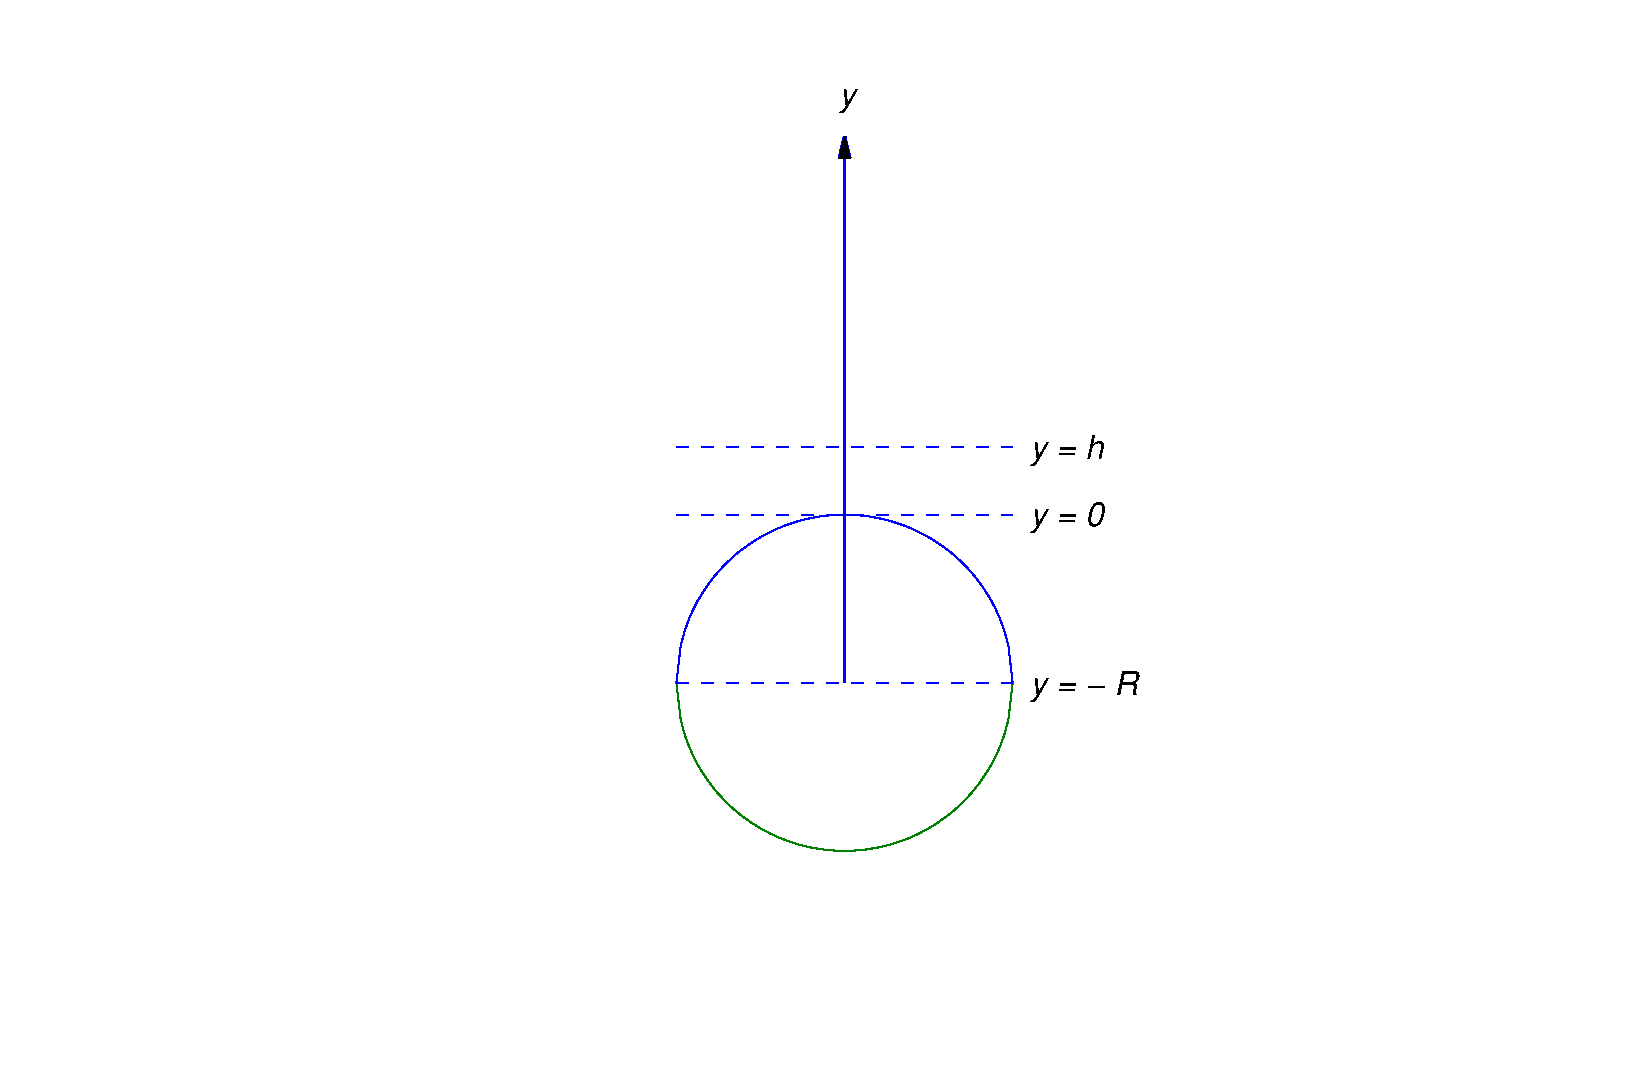
\includegraphics[bb=-78 148 689 643,width=5.67in,height=3.66in,keepaspectratio]{fig040305}
\color{blue}
  \caption{Escape velocity}
  \label{figure:4.3.5}
\end{figure}

 Since $F=-mg$ when $y=0$, setting $y=0$ in
(\ref{eq:4.3.18}) yields
$$
-mg=-{K\over R^2};
$$
 therefore $K=mgR^2$ and (\ref{eq:4.3.18}) can be written more
specifically as
\begin{equation} \label{eq:4.3.19}
F=-{mgR^2\over(y+R)^2}.
\end{equation}

From Newton's second law of motion,
$$
F=m{d^2y\over dt^2},
$$
so (\ref{eq:4.3.19}) implies that
\begin{equation} \label{eq:4.3.20}
{d^2y\over dt^2}=-{gR^2\over(y+R)^2}.
\end{equation}

We'll show that there's a number $v_e$, called the {\color{blue}\it
escape
velocity\/}, with these properties:

\begin{enumerate}
\item If $v_0\ge v_e$ then $v(t)>0$ for all $t>0$, and the vehicle
continues to climb for all $t>0$; that is, it ``escapes'' Earth.
(Is it really so obvious that $\lim_{t\to\infty}y(t)=\infty$
in this case? For a proof, see Exercise~\ref{exer:4.3.20}.)
\item  If $v_0<v_e$  then  $v(t)$   decreases to zero and becomes negative.
Therefore
 the vehicle attains a  maximum
altitude  $y_m$ and
falls back to Earth.
 \end{enumerate}

Since
(\ref{eq:4.3.20}) is second order, we can't solve it by methods discussed
so far. However, we're concerned with $v$ rather than $y$, and $v$ is
easier to find. Since $v=y'$ the chain rule implies that
$$
{d^2y\over dt^2}={dv\over dt}={dv\over dy}{dy\over dt}=v{dv\over dy}.
$$
 Substituting this into (\ref{eq:4.3.20}) yields the first order
separable equation
\begin{equation} \label{eq:4.3.21}
v{dv\over dy}=-{gR^2\over(y+R)^2}.
\end{equation}
When $t=0$, the velocity is $v_0$ and the altitude is $h$. Therefore
we can
obtain $v$ as a function of $y$ by solving the initial value problem
$$
v{dv\over dy}=-{gR^2\over(y+R)^2},\quad  v(h)=v_0.
$$

Integrating (\ref{eq:4.3.21}) with respect to $y$ yields
\begin{equation} \label{eq:4.3.22}
{v^2\over 2}={gR^2\over y+R}+c.
\end{equation}
 Since $v(h)=v_0$,
$$
c={v_0^2\over 2}-{gR^2\over h+R},
$$
 so (\ref{eq:4.3.22}) becomes
\begin{equation} \label{eq:4.3.23}
{v^2\over 2}={gR^2\over y+R}+\left({v_0^2\over 2}-
{gR^2\over h+R}\right).
\end{equation}
If
$$
v_0 \ge\left({2gR^2\over h+R}\right)^{1/2},
$$
 the parenthetical expression in (\ref{eq:4.3.23})  is nonnegative,
 so $v(y)>0$ for $y>h$. This proves that there's an escape
velocity $v_e$. We'll now prove that
$$
v_e=\left({2gR^2\over h+R}\right)^{1/2}
$$
by showing that the vehicle falls back to Earth if
\begin{equation} \label{eq:4.3.24}
v_0 <\left({2gR^2\over h+R}\right)^{1/2}.
\end{equation}
If (\ref{eq:4.3.24})  holds then  the parenthetical expression in
(\ref{eq:4.3.23})
is negative and the vehicle will attain a maximum altitude $y_m>h$
that satisfies the equation
$$
0={gR^2\over y_m+R}+\left({v_0^2\over 2}-
{gR^2\over h+R}\right).
$$
The velocity will be zero at the maximum  altitude, and the object will
then fall to Earth under the influence of gravity.

\exercises
Except where directed otherwise, assume that the magnitude of the
gravitational force on an object with mass $m$ is constant and equal
to $mg$. In exercises involving vertical motion take the upward
direction to be positive.

\begin{exerciselist}

\item\label{exer:4.3.1}
A firefighter  who weighs 192 lb slides down an infinitely long
fire pole
that exerts a frictional resistive force with magnitude proportional
to his speed, with $k=2.5$ lb-s/ft. Assuming that he starts from
rest, find his velocity as a function of time and find his terminal
velocity.

\item\label{exer:4.3.2}
A firefighter who weighs 192 lb slides down an infinitely long
fire pole
that exerts a frictional resistive force with magnitude proportional
to her speed, with constant of proportionality $k$. Find $k$, given
that her terminal velocity is -16 ft/s, and then find her velocity
$v$ as a function of $t$. Assume that she starts from rest.

\item\label{exer:4.3.3}
A boat weighs 64,000 lb. Its propellor produces a constant thrust of
50,000 lb and the water exerts a resistive force with magnitude
proportional to the speed, with $k=2000$ lb-s/ft. Assuming that the
boat starts from rest, find its velocity as a function of time, and
find its terminal velocity.

\item\label{exer:4.3.4}
A constant horizontal force of 10 N pushes a 20 kg-mass through a
medium that resists its motion with .5 N for every m/s of speed. The
initial velocity of the mass is 7 m/s in the direction opposite to
the direction of the applied force. Find the velocity of the mass for
$t > 0$.

\item\label{exer:4.3.5}
A stone weighing 1/2 lb is thrown upward from an initial height of 5
ft with an initial speed of 32 ft/s. Air resistance is
proportional to speed, with $k=1/128$ lb-s/ft. Find the
maximum height attained by the stone.

\item\label{exer:4.3.6}
A 3200-lb car is moving at 64 ft/s down a 30-degree grade when it
runs out of fuel. Find its velocity after that if friction exerts a
resistive force with magnitude proportional to the square of the
speed, with $k=1\ \mbox{lb-s}^2/{\mbox ft}^2$. Also find its
terminal velocity.

\item\label{exer:4.3.7}
A 96 lb weight is dropped from rest in a medium that exerts a
resistive force with magnitude proportional to the speed. Find its
velocity as a function of time if its terminal velocity is -128
ft/s.

\item\label{exer:4.3.8}
An object with mass $m$ moves vertically through a medium that exerts
a resistive force with magnitude proportional to the  speed. Let
$y=y(t)$ be the
altitude of the object at time $t$, with $y(0)=y_0$. Use the results
of Example~\ref{example:4.3.1} to show that
$$
 y(t)=y_0+{m\over k}(v_0-v-gt).
$$

\item\label{exer:4.3.9}
An object with mass $m$ is launched vertically upward with initial
velocity $v_0$ from Earth's surface ($y_0=0$) in a medium that exerts
a resistive force with magnitude proportional to the speed. Find the
time $T$ when the object attains its maximum altitude $y_m$. Then use
the result of Exercise~\ref{exer:4.3.8} to find $y_m$.

\item\label{exer:4.3.10}
An object weighing 256 lb is dropped from rest in a medium that
exerts a resistive force with magnitude proportional to the square of
the speed. The magnitude of the resisting force is 1 lb when $|v|=4\
\mbox{ft/s}$. Find $v$ for $t > 0$, and find its terminal
velocity.

\item\label{exer:4.3.11}
An object with mass $m$ is given an initial velocity $v_0\le0$ in
a medium that exerts
a resistive force with magnitude proportional to the square of the
speed. Find the velocity of the object for $t > 0$, and find its
terminal velocity.

\item\label{exer:4.3.12}
An object with mass $m$ is launched vertically upward with initial
velocity $v_0$ in a medium that exerts a resistive force
with magnitude  proportional to the square of the  speed.

\begin{alist}
\item %(a)
Find the time $T$ when the object reaches its maximum
altitude.
\item %(b)
Use the result of Exercise~\ref{exer:4.3.11} to find the velocity of the
object for $t > T$.
\end{alist}

\item\label{exer:4.3.13} \Lex
An object with mass $m$ is given an  initial velocity $v_0\le0$
in a medium that exerts a resistive force of the form
 $a|v|/(1+|v|)$, where  $a$ is positive constant.

\begin{alist}
\item % (a)
Set up a differential equation for the speed of the object.
\item % (b)
Use your favorite numerical method to solve the equation you found in
\part{a}, to convince yourself that there's  a unique number $a_0$ such
that $\lim_{t\to\infty}s(t)=\infty$ if $a\le a_0$ and
$\lim_{t\to\infty}s(t)$ exists (finite) if $a>a_0$. (We say that $a_0$
is the {\color{blue}\it bifurcation value\/} of $a$.) Try to find $a_0$ and
$\lim_{t\to\infty}s(t)$ in the case where $a>a_0$.
\hint{See Exercise~$\ref{exer:4.3.14}$.}
\end{alist}

\item\label{exer:4.3.14}
An object of mass $m$ falls in a medium that exerts a resistive force
$f=f(s)$, where $s=|v|$ is the speed of the object. Assume that
$f(0)=0$ and $f$ is strictly increasing and differentiable on
$(0,\infty)$.
\begin{alist}
\item % (a)
Write a differential equation for the speed $s=s(t)$ of the object.
Take it as given that all solutions of this equation with $s(0)\ge0$
are defined for all $t>0$ (which makes good sense on physical
grounds).
\item % (b)
Show that if $\lim_{s\to\infty}f(s)\le mg$ then
$\lim_{t\to\infty}s(t)=\infty$.
\item % (c)
Show that if $\lim_{s\to\infty}f(s)>mg$ then
$\lim_{t\to\infty}s(t)=s_T$ (terminal speed), where $f(s_T)=mg$.
\hint{Use Theorem~\ref{thmtype:2.3.1}}.
\end{alist}

\item\label{exer:4.3.15}
A 100-g mass with initial velocity $v_0\le0$ falls in a medium that
exerts a resistive force proportional to the fourth power of the
speed. The resistance is $.1$ N if the speed is 3 m/s.

\begin{alist}
\item % (a)
Set up the initial value problem for the velocity $v$ of the mass for
$t>0$.
\item % (b)
Use Exercise~\ref{exer:4.3.14}(c) to determine the terminal velocity of
the object.
\item % (c)
\Cex
To confirm your answer to \part{b},  use one of the numerical methods  studied
in Chapter~3 to compute  approximate solutions on $[0,1]$
(seconds) of the initial value problem of \part{a}, with initial values
$v_0=0$, $-2$, $-4$, \dots, $-12$. Present your results in graphical form
similar to Figure~\ref{figure:4.3.3}.
\end{alist}

\item\label{exer:4.3.16}
A 64-lb object with initial velocity $v_0\le0$ falls through a dense
fluid that exerts a resistive force proportional to the square root of
the speed. The resistance is $64$ lb if the speed is 16 ft/s.

\begin{alist}
\item % (a)
Set up the initial value problem for the velocity $v$ of the mass for
$t>0$.
\item % (b)
Use Exercise~\ref{exer:4.3.14}(c) to determine the terminal velocity of
the object.
\item % (c)
\Cex
To confirm your answer to \part{b}, use one of the numerical methods
studied in Chapter~3 to compute approximate
solutions on
$[0,4]$ (seconds) of the initial value problem of \part{a}, with
initial values $v_0=0$, $-5$, $-10$, \dots, $-30$. Present your results in
graphical form similar to Figure~\ref{figure:4.3.3}.
\end{alist}

\exercisetext{In Exercises \ref{exer:4.3.17}-\ref{exer:4.3.20}, assume
that the
force due to gravity is given by Newton's law of gravitation. Take the
upward direction to be positive.}

\item\label{exer:4.3.17}
A space probe is to be launched from a space station 200
miles above Earth.  Determine its escape velocity in
miles/s.  Take Earth's radius to be 3960 miles.

\item\label{exer:4.3.18}
A space vehicle is to be launched from the moon, which has a
radius of about 1080 miles.  The acceleration due to
gravity at the surface of the moon is about $5.31$
ft/s$^2$.  Find the escape velocity in miles/s.

\item\label{exer:4.3.19}
\begin{alist}
\item %(a)
Show that Eqn.~(\ref{eq:4.3.23})  can be rewritten as
$$
v^2={h-y\over y+R} v^2_e+v_0^2.
$$
\item %(b)
Show that if $v_0=\rho v_e$ with $ 0\le \rho < 1$, then
the maximum altitude $y_m$ attained by the space
vehicle is
$$
y_m={h+R\rho^2\over 1-\rho^2}.
$$
\item %(c)
By requiring that $v(y_m)=0$, use Eqn.~(\ref{eq:4.3.22}) to
deduce that if $v_0 < v_e$ then
$$
|v|=v_e\left[{(1-\rho^2)(y_m-y)\over y+R}\right]^{1/2},
$$
where $y_m$ and $\rho$ are as defined in \part{b} and
$y \ge h$.
\item %(d)
Deduce from \part{c} that if $v < v_e$,  the vehicle takes
equal times to climb from $y=h$ to $y=y_m$ and to
fall back from $y=y_m$ to $y=h$.
\end{alist}

\item\label{exer:4.3.20}
In the situation considered in the discussion of escape velocity, show
that $\lim_{t\to\infty}y(t)=\infty$ if $v(t)>0$ for all $t>0$.

\hint{Use a proof by contradiction. Assume that there's a number
$y_m$ such that $y(t)\le y_m$ for all $t>0$. Deduce from this that
there's positive number $\alpha$ such that $y''(t)\le-\alpha$ for all
$t\ge0$. Show that this contradicts the assumption that $v(t)>0$ for
all $t>0$.}
\end{exerciselist}


\section{Autonomous Second Order Equations}

\noindent
A second order differential equation that can be written as
\begin{equation} \label{eq:4.4.1}
y''=F(y,y')
\end{equation}
where $F$ is independent of $t$, is said to be {\color{blue}\it autonomous\/}.
An autonomous second order equation can be converted into a first
order equation relating $v=y'$ and $y$. If we let $v=y'$,
\eqref{eq:4.4.1} becomes
\begin{equation} \label{eq:4.4.2}
v'=F(y,v).
\end{equation}
Since
\begin{equation} \label{eq:4.4.3}
v'={dv\over dt}={dv\over dy}{dy\over dt}=v{dv\over dy},
\end{equation}
\eqref{eq:4.4.2} can be rewritten as
\begin{equation} \label{eq:4.4.4}
v{dv\over dy}=F(y,v).
\end{equation}
The integral curves of \eqref{eq:4.4.4} can be plotted in the $(y,v)$
plane, which is called the
\href{https://mathshistory.st-andrews.ac.uk/Biographies/Poincare/}
{\color{blue}\it Poincar\'e
 phase plane\/} of \eqref{eq:4.4.1}. If $y$ is a solution of
\eqref{eq:4.4.1}
then $y=y(t)$, $v=y'(t)$ is a parametric equation for an integral curve
of \eqref{eq:4.4.4}. We'll call these integral curves {\color{blue}\it
trajectories\/} of \eqref{eq:4.4.1}, and we'll call
\eqref{eq:4.4.4} the {\color{blue}\it phase plane equivalent\/} of \eqref{eq:4.4.1}.

In this section we'll consider  autonomous equations
that can be written as
\begin{equation} \label{eq:4.4.5}
y''+q(y,y')y'+p(y)=0.
\end{equation}
Equations of this form often arise in applications of Newton's second
law of motion. For example, suppose  $y$ is the displacement of a
moving object with mass $m$. It's  reasonable to think of two
types of time-independent forces acting on the object. One type - such
as gravity - depends only on position. We could write such a force as
$-mp(y)$. The second type - such as atmospheric resistance or friction
- may depend on position and velocity. (Forces that depend on velocity
are called {\color{blue}\it damping\/} forces.) We  write this force as
$-mq(y,y')y'$, where $q(y,y')$ is usually a positive function and
we've put the factor $y'$ outside  to make it
explicit that the force
is in the direction opposing the motion. In this case Newton's, second
law of motion leads to \eqref{eq:4.4.5}.

The phase plane equivalent of \eqref{eq:4.4.5} is
\begin{equation} \label{eq:4.4.6}
v{dv\over dy}+q(y,v)v+p(y)=0.
\end{equation}
Some  statements that we'll be making about the properties of
\eqref{eq:4.4.5} and \eqref{eq:4.4.6} are intuitively reasonable, but
difficult to prove.
Therefore our presentation in this section will be informal: we'll
just say things without proof, all of which are true if we assume that
$p=p(y)$ is continuously differentiable for all $y$ and $q=q(y,v)$ is
continuously differentiable for all $(y,v)$.
 We begin with the following statements:

\begin{itemize}
\item{\bf Statement 1.} If $y_0$ and $v_0$ are arbitrary real numbers then
\eqref{eq:4.4.5} has a unique solution on $(-\infty,\infty)$ such that
$y(0)=y_0$ and $y'(0)=v_0$.

\item{\bf Statement 2.)} If $y=y(t)$ is a solution of \eqref{eq:4.4.5}
and
$\tau$ is any constant then $y_1=y(t-\tau)$ is also a solution of
\eqref{eq:4.4.5}, and $y$ and $y_1$ have the same trajectory.

\item{\bf Statement 3.}   If two solutions $y$ and $y_1$ of
\eqref{eq:4.4.5} have the same trajectory then  $y_1(t)=y(t-\tau)$
for some constant $\tau$.

\item{\bf Statement 4.} Distinct trajectories of \eqref{eq:4.4.5} can't
intersect; that is, if two trajectories of \eqref{eq:4.4.5}
intersect,  they are identical.

\item{\bf Statement 5.} If the trajectory of a solution of
\eqref{eq:4.4.5}
is a closed curve then  $(y(t),v(t))$ traverses the
trajectory in a finite time $T$, and the solution is periodic with
period $T$; that is, $y(t+T)=y(t)$ for all $t$ in $(-\infty,\infty)$.
\end{itemize}

If $\overline y$ is a constant such that $p(\overline y)=0$ then
$y\equiv\overline y$ is a constant solution of \eqref{eq:4.4.5}. We say
that $\overline y$ is an {\color{blue}\it equilibrium\/} of \eqref{eq:4.4.5} and
 $(\overline y,0)$ is a {\color{blue}\it critical point\/} of the phase plane
equivalent equation \eqref{eq:4.4.6}. We say that the equilibrium and
the critical point are {\color{blue}\it stable\/} if, for any given $\epsilon>0$
{\color{blue}\it no matter how small\/}, there's a $\delta>0$,
{\color{blue}\it
sufficiently small\/}, such that if
$$
\sqrt{(y_0-\overline y)^2+v_0^2}<\delta
$$
then the  solution of the initial value problem
$$
y''+q(y,y')y'+p(y)=0,\quad y(0)=y_0,\quad y'(0)=v_0
$$
satisfies the inequality
$$
\sqrt{(y(t)-\overline y)^2+(v(t))^2}<\epsilon
$$
for all $t>0$. Figure~\ref{figure:4.4.1} illustrates the geometrical
interpretation of this definition in the Poincar\'e phase plane: if
$(y_0,v_0)$ is in the smaller shaded circle (with radius~$\delta$), then
$(y(t),v(t))$ must be in the larger circle (with
radius~$\epsilon$) for all $t>0$.

\begin{figure}[H]
  \centering
  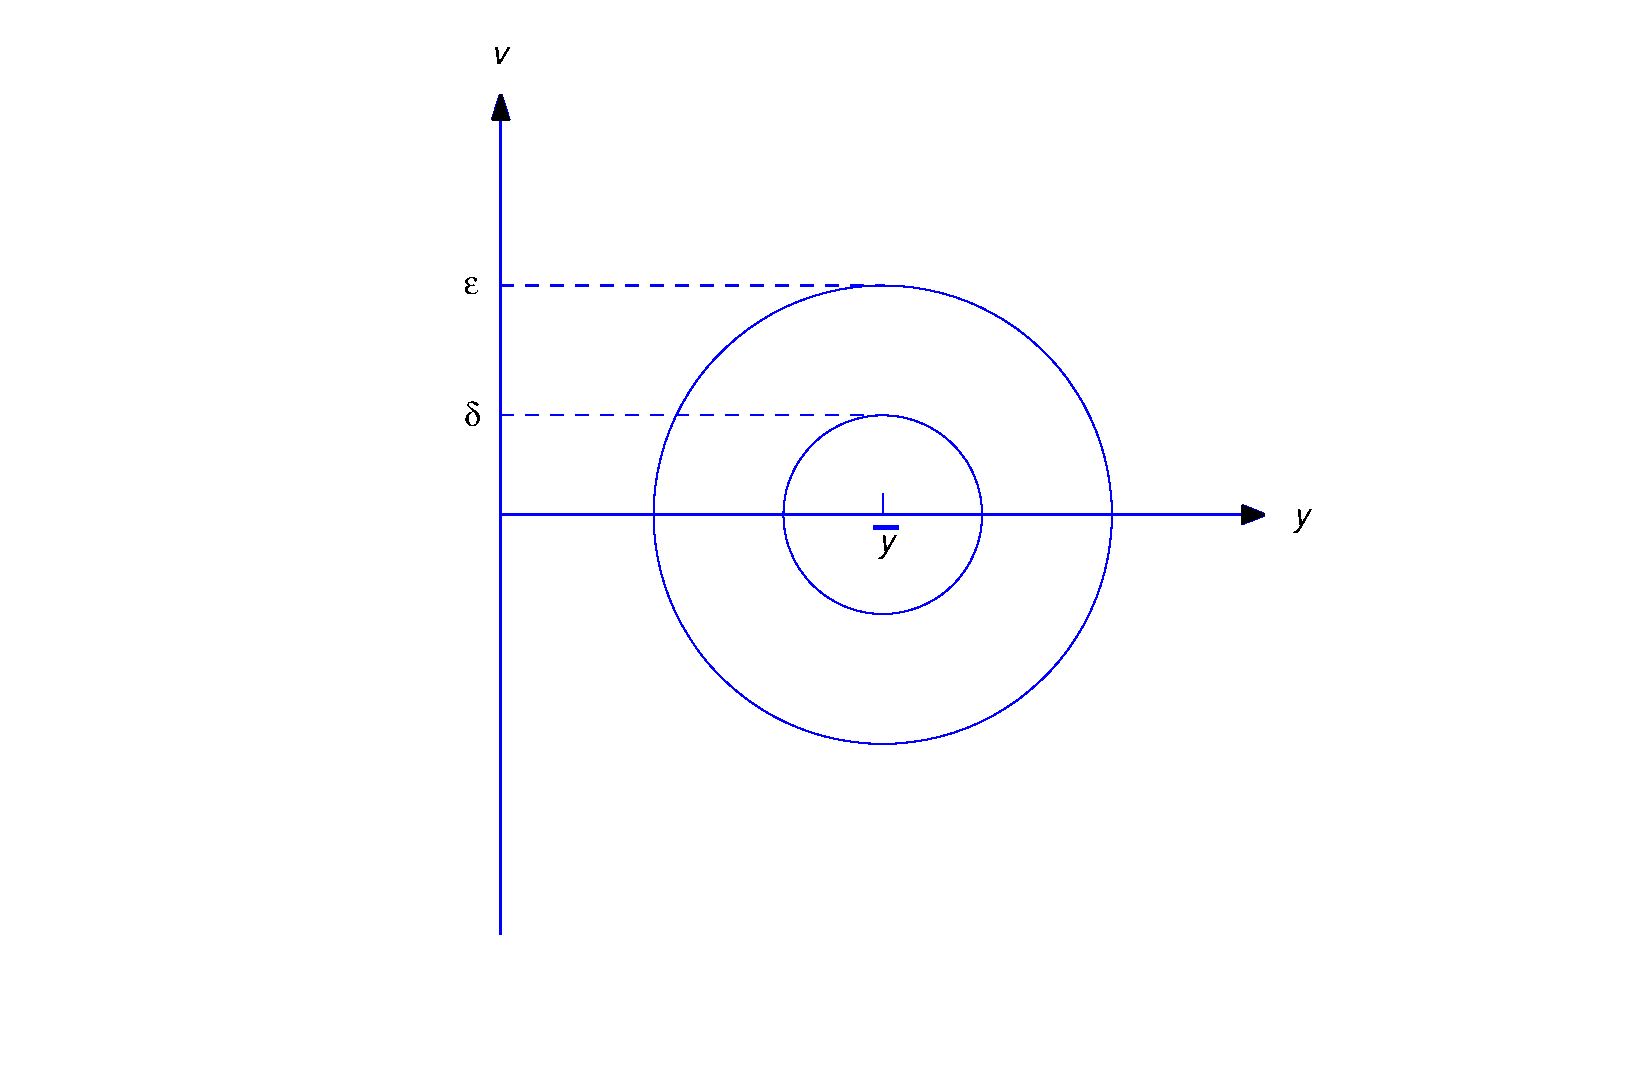
\includegraphics[bb=-78 148 689 643,width=5.67in,height=3.66in,keepaspectratio]{fig040401}
\color{blue}
\caption{Stability: if $(y_0,v_0)$ is in the smaller
circle  then $(y(t),v(t))$ is in the larger circle for all $t>0$}
  \label{figure:4.4.1}
\end{figure}

If an equilibrium and the associated critical point are not stable, we
say they are {\color{blue}\it unstable\/}. To see if you really understand what
{\color{blue}\it stable\/} means, try to give a direct definition of {\color{blue}\it
unstable\/}
(Exercise~\ref{exer:4.4.22}). We'll illustrate both definitions in
the following examples.

\boxit{The Undamped Case}

\noindent
We'll begin with the case where $q\equiv0$, so  \eqref{eq:4.4.5}
reduces to
 \begin{equation} \label{eq:4.4.7}
y''+p(y)=0.
\end{equation}
We say that this equation - as well as any physical situation
that it may model - is {\color{blue}\it undamped\/}.
The phase plane equivalent of \eqref{eq:4.4.7} is  the
separable equation
$$
v{dv\over dy}+p(y)=0.
$$
 Integrating this  yields
\begin{equation} \label{eq:4.4.8}
{v^2\over2}+P(y)=c,
\end{equation}
where $c$ is a constant of integration and $P(y)=\int p(y)\,dy$ is an
antiderivative of $p$.

If \eqref{eq:4.4.7} is the equation of motion of an object of
mass $m$, then
 $mv^2/2$ is the kinetic energy and $mP(y)$ is the
potential energy of the object;   thus, \eqref{eq:4.4.8} says that the
total
energy of the object remains constant, or is {\color{blue}\it conserved\/}. In
particular, if a trajectory passes through a given point $(y_0,v_0)$
then
$$
c={v_0^2\over2}+P(y_0).
$$

\begin{example}$[$The Undamped Spring - Mass
System$]\,$\label{example:4.4.1}\rm
 Consider an object with mass $m$ suspended from a
spring and moving vertically. Let $y$ be the displacement of the
object from the position it occupies when suspended at rest from the
spring (Figure~\ref{figure:4.4.2}).

\begin{figure}[H]
  \centering
  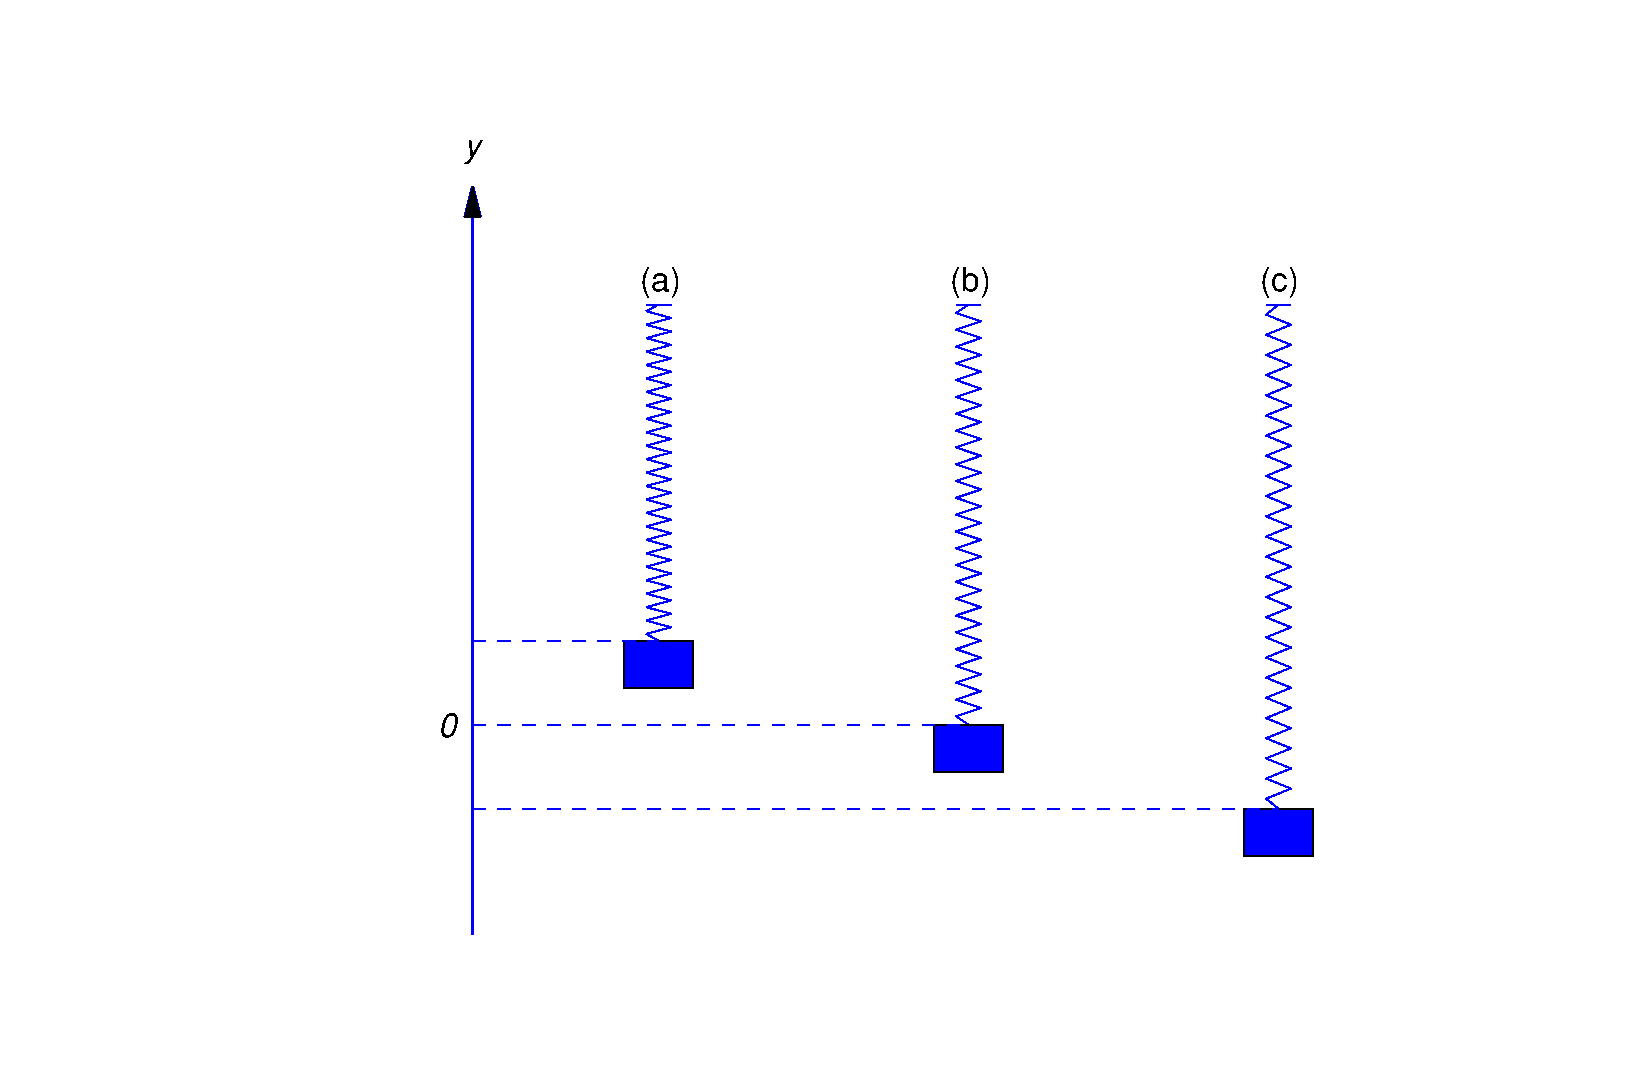
\includegraphics[bb=-78 148 689 643,width=5.67in,height=3.66in,keepaspectratio]{fig040402}
\color{blue}
  \caption{\,\part{a}  $y>0$   \, \part{b}  $y=0$   \, \part{c}  $y<0$}
  \label{figure:4.4.2}
\end{figure}

Assume that if the length of the spring is changed by an amount
$\Delta L$ (positive or negative), then the spring exerts an opposing
force with magnitude $k|\Delta L|$, where k is a positive constant. In
Section~6.1 it will be shown that if the mass of the spring
is negligible compared to $m$ and no other forces act on the object then
Newton's second law of motion implies that
\begin{equation} \label{eq:4.4.9}
my''=-ky,
\end{equation}
which can be written in the form \eqref{eq:4.4.7} with $p(y)=ky/m$. This
equation can be solved easily by a method that we'll study in
Section~5.2, but that method isn't available here. Instead,
we'll consider the phase plane equivalent of \eqref{eq:4.4.9}.

From \eqref{eq:4.4.3}, we can rewrite \eqref{eq:4.4.9} as the separable
equation
$$
 mv{dv\over dy}=-ky.
$$
Integrating this  yields
$$
{mv^2\over2}=-{ky^2\over2}+c,
$$
which implies that
\begin{equation} \label{eq:4.4.10}
mv^2+ky^2=\rho
\end{equation}
($\rho=2c$). This defines an ellipse in the Poincar\'e phase plane
(Figure~\ref{figure:4.4.3}).

\begin{figure}[tbp]
  \centering
  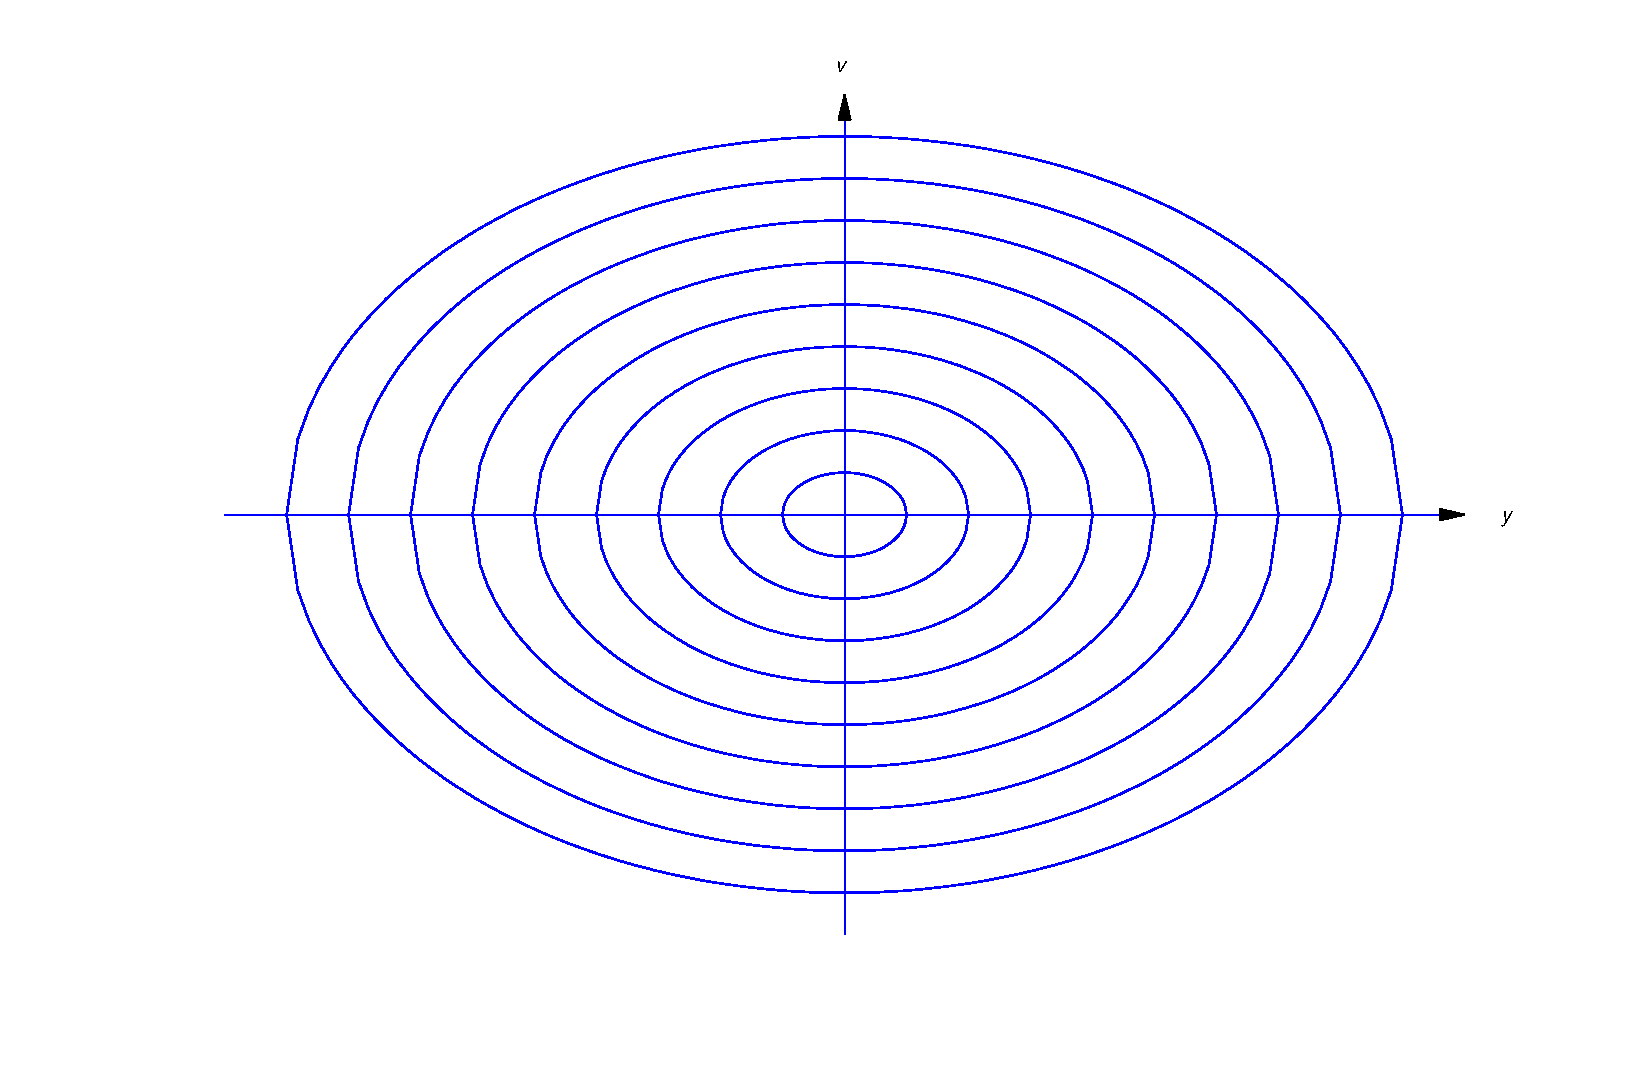
\includegraphics[bb=-78 148 689 643,width=5.67in,height=3.66in,keepaspectratio]{fig040403}
\color{blue}
\caption{Trajectories of  $my''+ky=0$}
  \label{figure:4.4.3}
\end{figure}

We can identify $\rho$ by setting $t=0$ in \eqref{eq:4.4.10};   thus,
$\rho=mv_0^2+ky_0^2$, where $y_0=y(0)$ and $v_0=v(0)$. To determine
the maximum and minimum values of $y$ we set $v=0$ in \eqref{eq:4.4.10};
thus,
\begin{equation} \label{eq:4.4.11}
y_{\max}=R\mbox{\quad and \quad}
y_{\min}=-R,\mbox{\quad with } R=\sqrt{\rho\over k}.
\end{equation}
Equation~\eqref{eq:4.4.9} has exactly one equilibrium, $\overline y=0$,
and
it's stable. You can see intuitively why this is so: if the object is
displaced in either direction from  equilibrium, the spring tries
to bring it back.

In this case we can find $y$ explicitly as a function of $t$. (Don't
expect this to happen in more complicated problems!) If $v>0$ on an
interval $I$,  \eqref{eq:4.4.10} implies that
$$
{dy\over dt}=v=\sqrt{\rho-ky^2\over m}
$$
on $I$. This is equivalent to
\begin{equation} \label{eq:4.4.12}
{\sqrt k\over\sqrt{\rho-ky^2}}{dy\over dt}=\omega_0,\mbox{\quad where
\quad}
\omega_0=\sqrt{k\over m}.
\end{equation}
Since
$$
\int{\sqrt k\,dy\over\sqrt{\rho-ky^2}}=\sin^{-1}\left(\sqrt{k\over\rho
}y\right)+c=\sin^{-1}\left(y\over R\right)+c
$$
(see \eqref{eq:4.4.11}), \eqref{eq:4.4.12} implies that that there's a
constant $\phi$ such that
$$
\sin^{-1}\left(y\over R\right)=\omega_0 t+\phi
$$
or
$$
y=R\sin(\omega_0 t+\phi)
$$
for all $t$ in $I$. Although we obtained this function by assuming that
$v>0$, you can easily verify that $y$ satisfies \eqref{eq:4.4.9} for all
values of $t$. Thus, the displacement varies periodically between $-R$
and $R$, with period $T=2\pi/\omega_0$ (Figure~\ref{figure:4.4.4}). (If
you've taken a course in elementary mechanics you may recognize this
as {\color{blue}\it simple harmonic motion\/}.)
\end{example}

\begin{figure}[tbp]
  \centering
  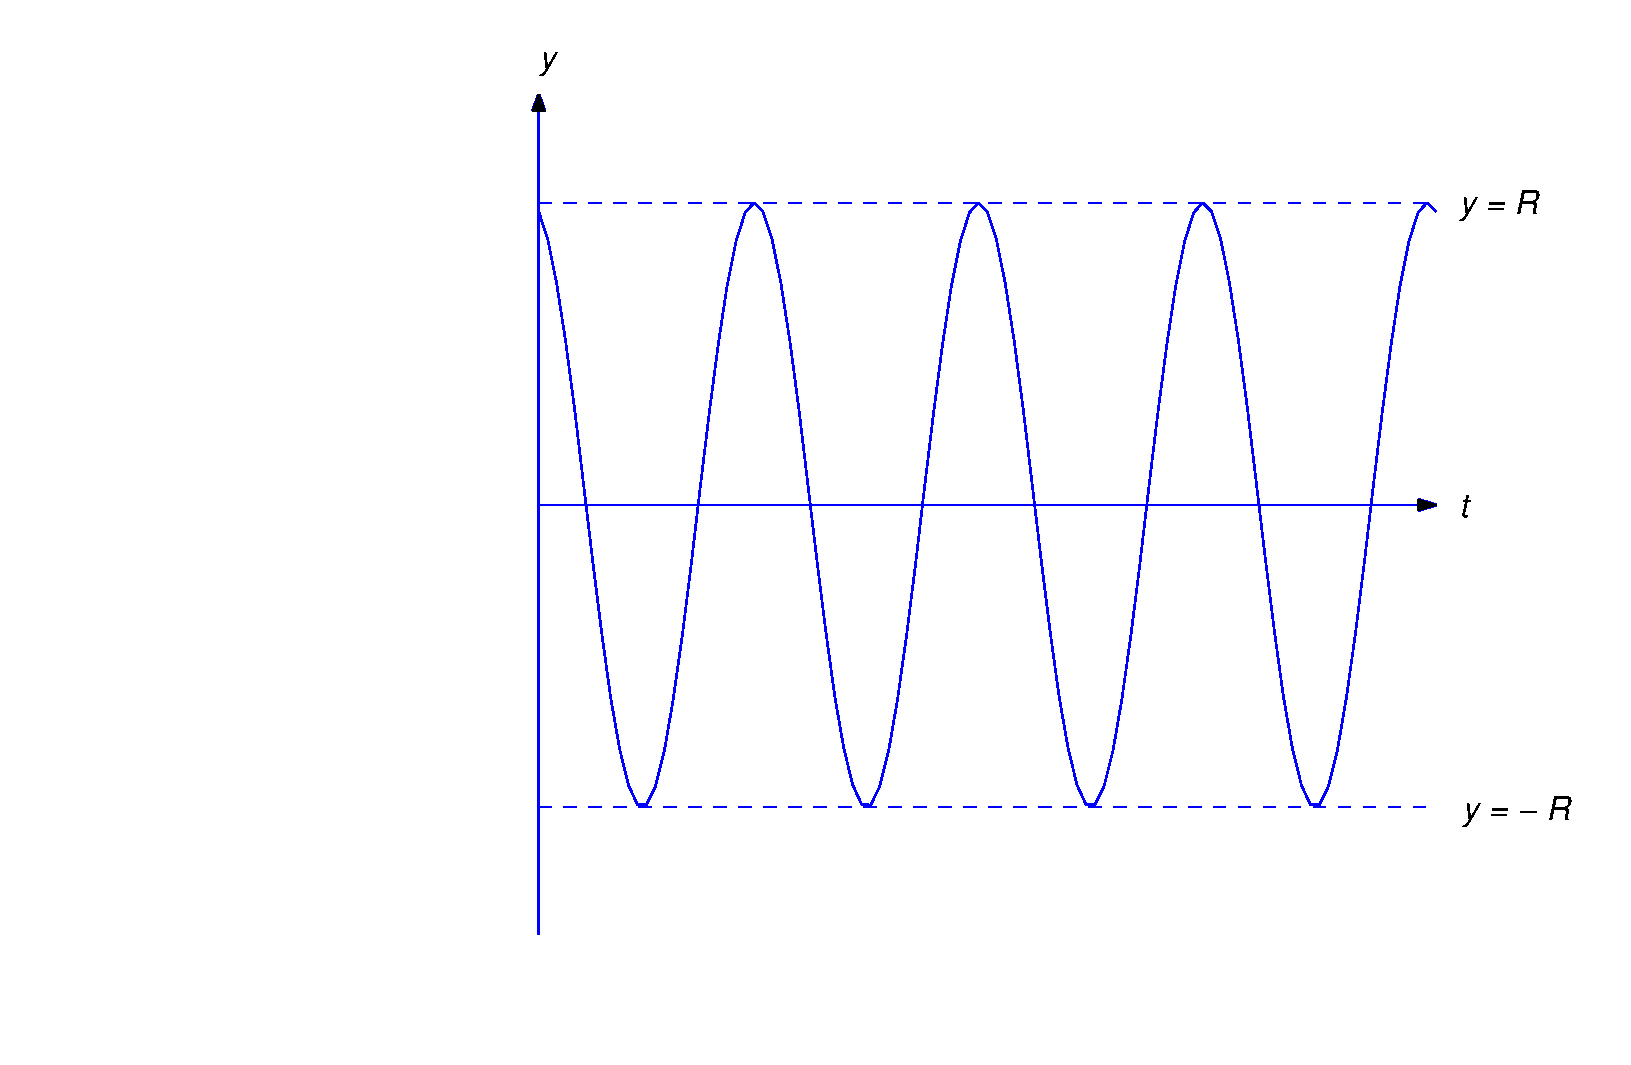
\includegraphics[bb=-78 148 689 643,width=5.67in,height=3.66in,keepaspectratio]{fig040404}
\color{blue}
\caption{$y=R\sin(\omega_0 t+\phi)$}
  \label{figure:4.4.4}
\end{figure}

\begin{example}$[$The Undamped Pendulum$]$\label{example:4.4.2}\rm
\, Now we
consider the motion of a pendulum with mass $m$, attached to the end
of a weightless rod with length $L$ that rotates on a frictionless
axle (Figure~\ref{figure:4.4.5}). We assume that there's no air
resistance.

Let $y$ be the angle measured from the rest position
(vertically downward) of the pendulum, as shown in
Figure~\ref{figure:4.4.5}. Newton's second law of motion says that the
product of $m$ and the tangential acceleration equals the tangential
component of the gravitational force;  therefore, from
Figure~\ref{figure:4.4.5},
$$
mLy''=-mg\sin y,
$$
or
\begin{equation} \label{eq:4.4.13}
y''=-{g\over L} \sin y.
\end{equation}

\begin{figure}[tbp]
  \centering
\scalebox{.5}{
  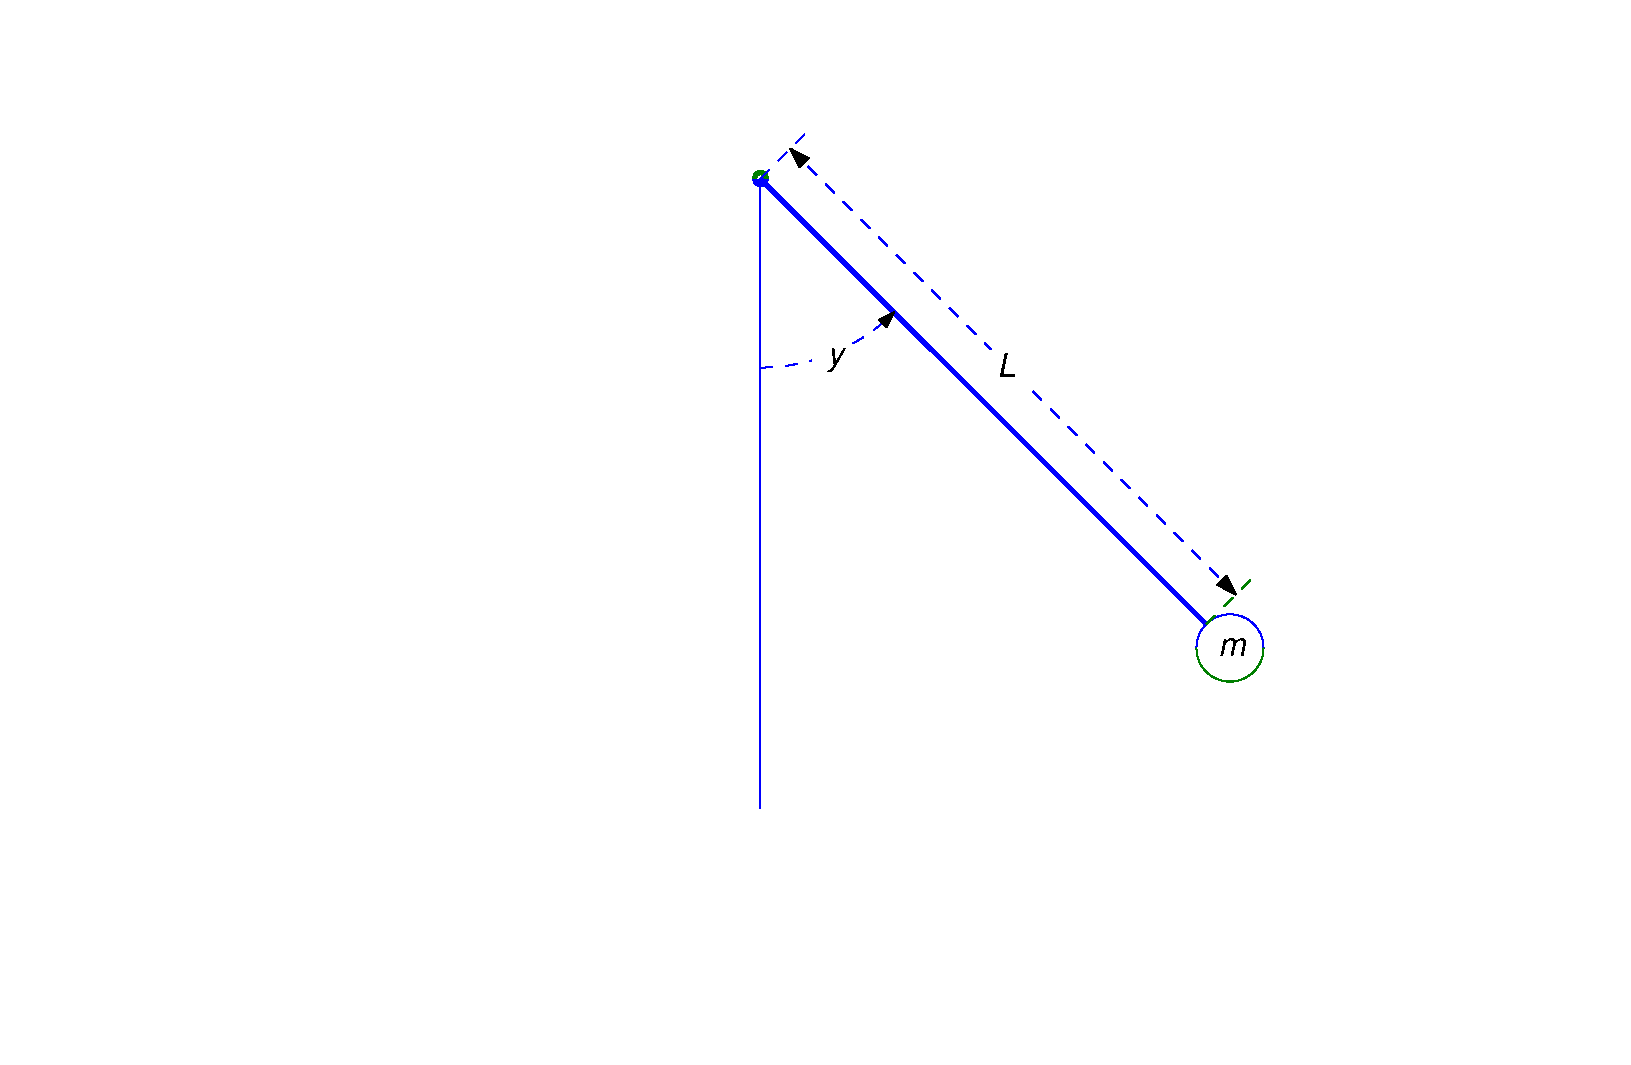
\includegraphics[bb=-78 148 689 643,width=5.67in,height=3.66in,keepaspectratio]{fig040405} }
\color{blue}
\caption{ The undamped pendulum}
  \label{figure:4.4.5}
\end{figure}

Since $\sin n\pi=0$ if $n$ is any integer,  \eqref{eq:4.4.13} has
infinitely many equilibria $\overline y_n=n\pi$. If $n$ is
even, the mass is directly below the axle
(Figure~\ref{figure:4.4.6}~\part{a}) and gravity opposes any deviation
from the equilibrium. However, if $n$ is odd, the mass is directly
above the axle (Figure~\ref{figure:4.4.6}~\part{b}) and gravity
increases any deviation from the equilibrium. Therefore we conclude
on physical grounds that $\overline y_{2m}=2m\pi$ is stable and
$\overline y_{2m+1}=(2m+1)\pi$ is unstable.

\begin{figure}[tbp]
  \centering
\scalebox{.5}{
  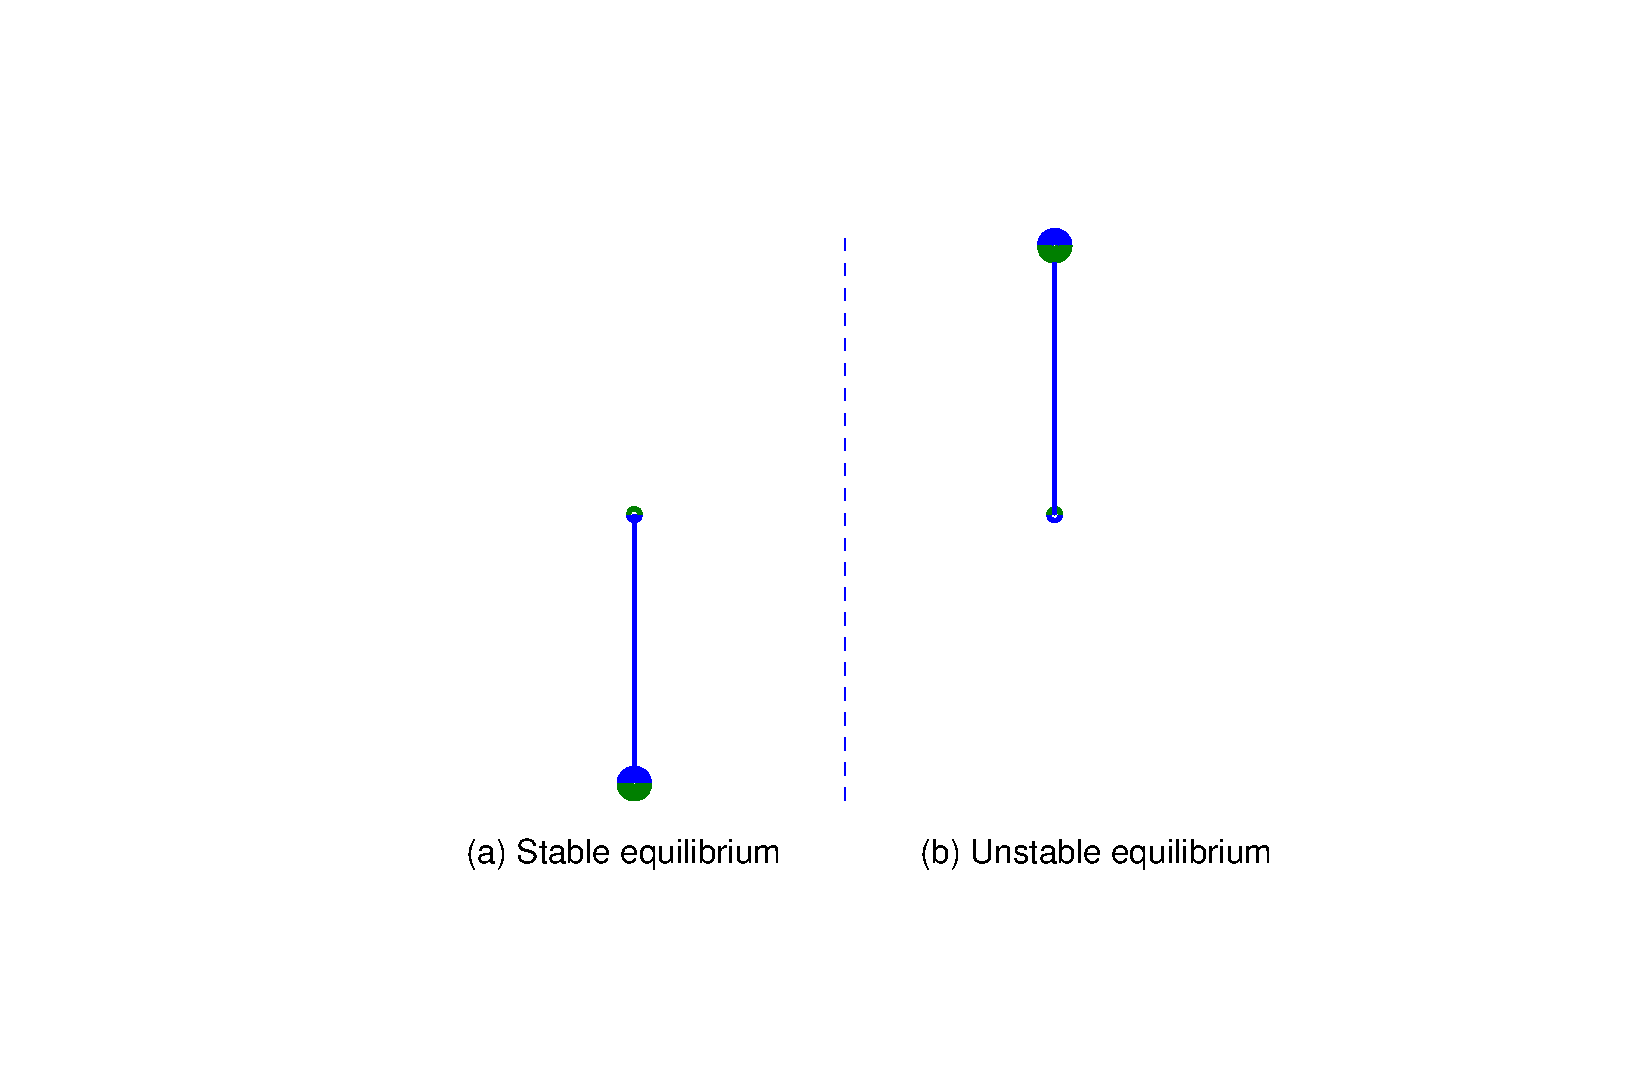
\includegraphics[bb=-78 148 689 643,width=5.67in,height=3.66in,keepaspectratio]{fig040406} }
\color{blue}
\caption{ \part{a}\, Stable equilibrium  \, \part{b}\, Unstable
equilibrium}
  \label{figure:4.4.6}
\end{figure}

The phase plane equivalent of \eqref{eq:4.4.13} is
$$
v{dv\over dy}=-{g\over L}\sin y,
$$
where $v=y'$ is the angular velocity of the pendulum. Integrating this
yields
\begin{equation} \label{eq:4.4.14}
{v^2\over2}={g\over L}\cos y+c.
\end{equation}
If $v=v_0$ when $y=0$, then
$$
c={v_0^2\over2}-{g\over L},
$$
so \eqref{eq:4.4.14} becomes
$$
{v^2\over2}={v_0^2\over2}-{g\over L}(1-\cos y)
={v_0^2\over2}-{2g\over L}\sin^2{y\over2},
$$
which is equivalent to
\begin{equation} \label{eq:4.4.15}
v^2=v_0^2-v_c^2\sin^2{y\over2},
\end{equation}
 where
$$
v_c=2\sqrt{g\over L}.
$$

The curves defined by \eqref{eq:4.4.15} are the trajectories of
\eqref{eq:4.4.13}. They are periodic with period $2\pi$ in $y$, which isn't
 surprising, since if $y=y(t)$ is a solution of \eqref{eq:4.4.13} then
so is $y_n=y(t)+2n\pi$ for any integer $n$. Figure~\ref{figure:4.4.7}
shows trajectories over the interval $[-\pi,\pi]$. From \eqref{eq:4.4.15},
you can see that if $|v_0|>v_c$ then $v$ is nonzero for all $t$, which
means that the object whirls in the same direction forever, as in
Figure~\ref{figure:4.4.8}. The trajectories associated with this
whirling motion are above the upper dashed curve and below the lower
dashed curve in Figure~\ref{figure:4.4.7}. You can also see from
\eqref{eq:4.4.15} that if $0<|v_0|<v_c$,then $v=0$ when $y=\pm y_{\max}$,
where
$$
y_{\max}=2\sin^{-1}(|v_0|/v_c).
$$
In this case the pendulum oscillates periodically between $-y_{\max}$
and $y_{\max}$, as shown in Figure~\ref{figure:4.4.9}. The
trajectories associated with this kind of motion are the ovals between
the dashed curves in Figure~\ref{figure:4.4.7}. It can be shown (see
Exercise~\ref{exer:4.4.21} for a partial proof) that the period of the
oscillation is
\begin{equation} \label{eq:4.4.16}
T=8\int_0^{\pi/2}{d\theta\over\sqrt{v_c^2-v_0^2\sin^2\theta}}.
\end{equation}
Although this integral can't be evaluated in terms of familiar
elementary functions, you can see that it's finite if $|v_0|<v_c$.

The dashed curves in Figure~\ref{figure:4.4.7} contain four
trajectories. The critical points $(\pi,0)$ and $(-\pi,0)$ are the
trajectories of the unstable equilibrium solutions $\overline
y=\pm\pi$.
The upper dashed curve connecting (but not including) them is obtained
from initial conditions of the form $y(t_0)=0$, $v(t_0)=v_c$. If $y$ is
any solution with this trajectory then
$$
\lim_{t\to\infty}y(t)=\pi\mbox{\quad and \quad}\lim_{t\to-\infty}y(t)=-\pi.
$$
The lower dashed curve connecting (but not including) them is obtained
from initial conditions of the form $y(t_0)=0$, $v(t_0)=-v_c$. If $y$
is any solution with this trajectory then
$$
\lim_{t\to\infty}y(t)=-\pi\mbox{\quad and \quad}\lim_{t\to-\infty}y(t)=\pi.
$$
Consistent with this, the integral \eqref{eq:4.4.16} diverges to $\infty$
if $v_0=\pm v_c$. (Exercise~\ref{exer:4.4.21}) .

Since the dashed curves separate trajectories of whirling solutions
from trajectories of oscillating solutions, each of these curves is
called a {\color{blue}\it separatrix\/}.

In general, if \eqref{eq:4.4.7} has both stable and unstable equilibria
then the separatrices are the curves given by \eqref{eq:4.4.8} that pass
through unstable critical points. Thus, if $(\overline y,0)$ is an
unstable critical point, then
\begin{equation} \label{eq:4.4.17}
{v^2\over 2}+P(y)=P(\overline y)
\end{equation}
\enlargethispage{30pt}
defines a separatrix passing through $(\overline y,0)$.
\end{example}

\newpage
\vspace*{-.2in}
\begin{figure}[H]
  \centering
\scalebox{.5}{
  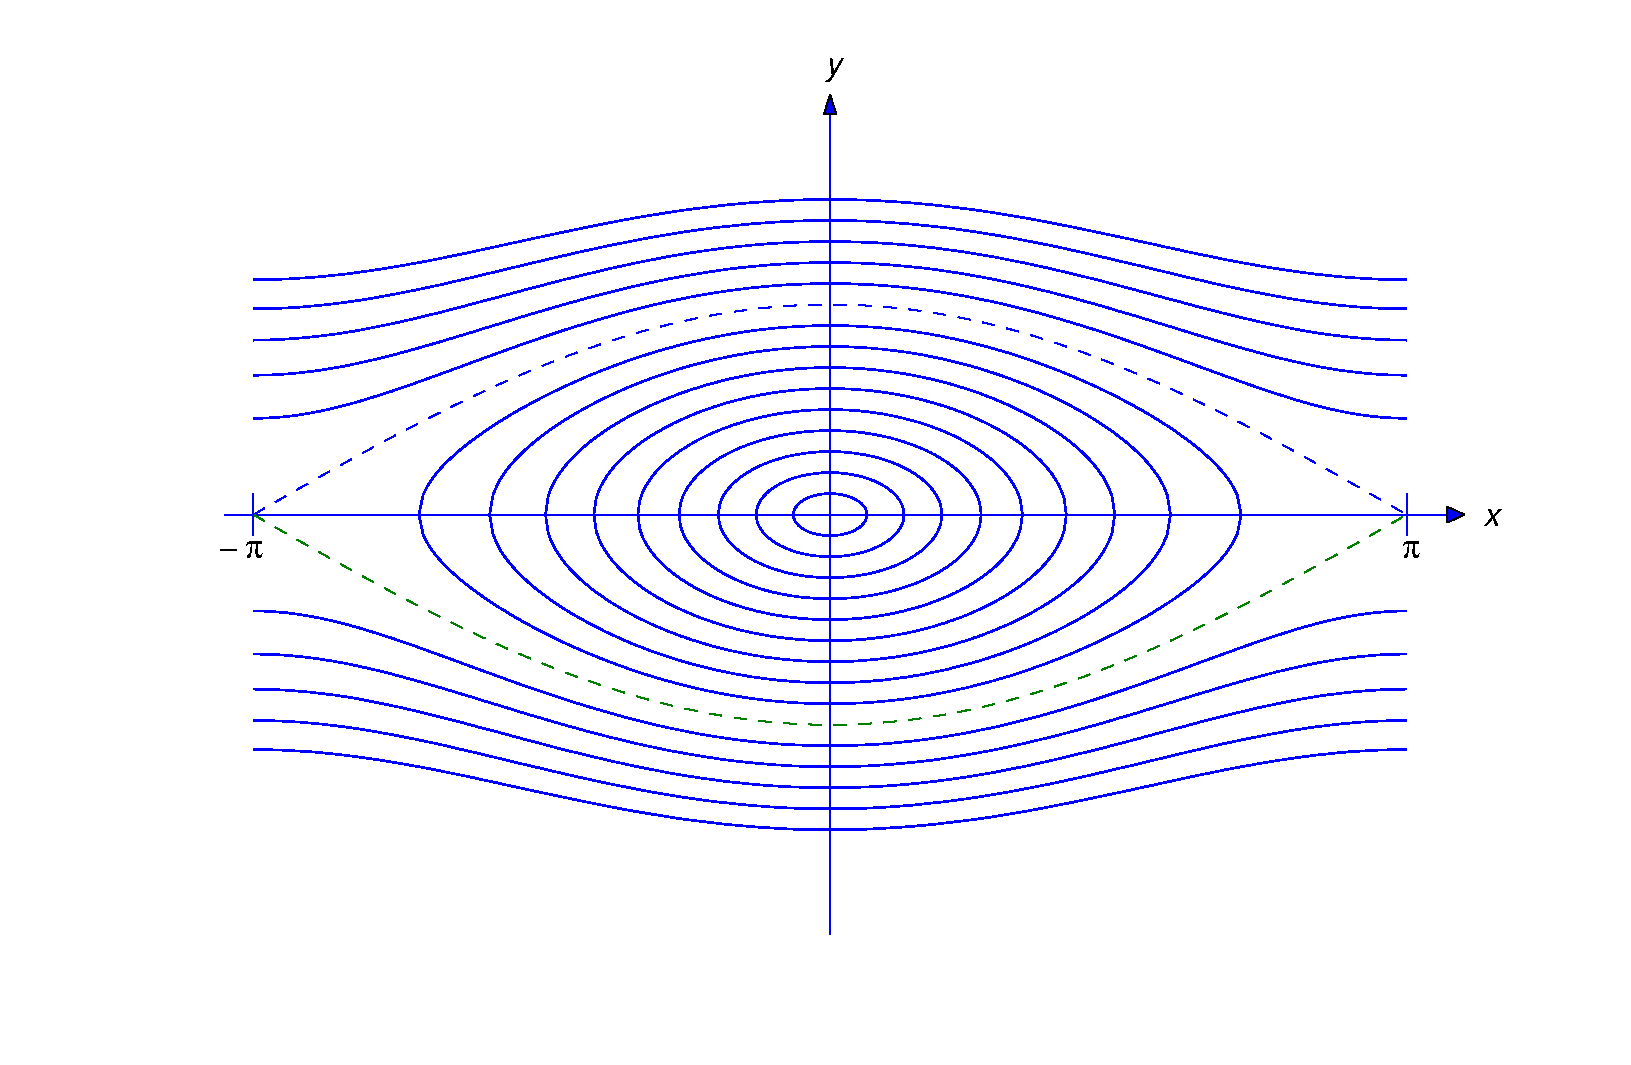
\includegraphics[bb=-78 148 689 643,width=5.67in,height=3.66in,keepaspectratio]{fig040407} }
\color{blue}
\caption{ Trajectories of the undamped pendulum}
  \label{figure:4.4.7}
\end{figure}

\vspace*{-25pt}
\begin{figure}[H]
%\begin{figure}[htbp]
\color{blue}
  \begin{minipage}[b]{0.5\linewidth}
    \centering
  \scalebox{.7}{
  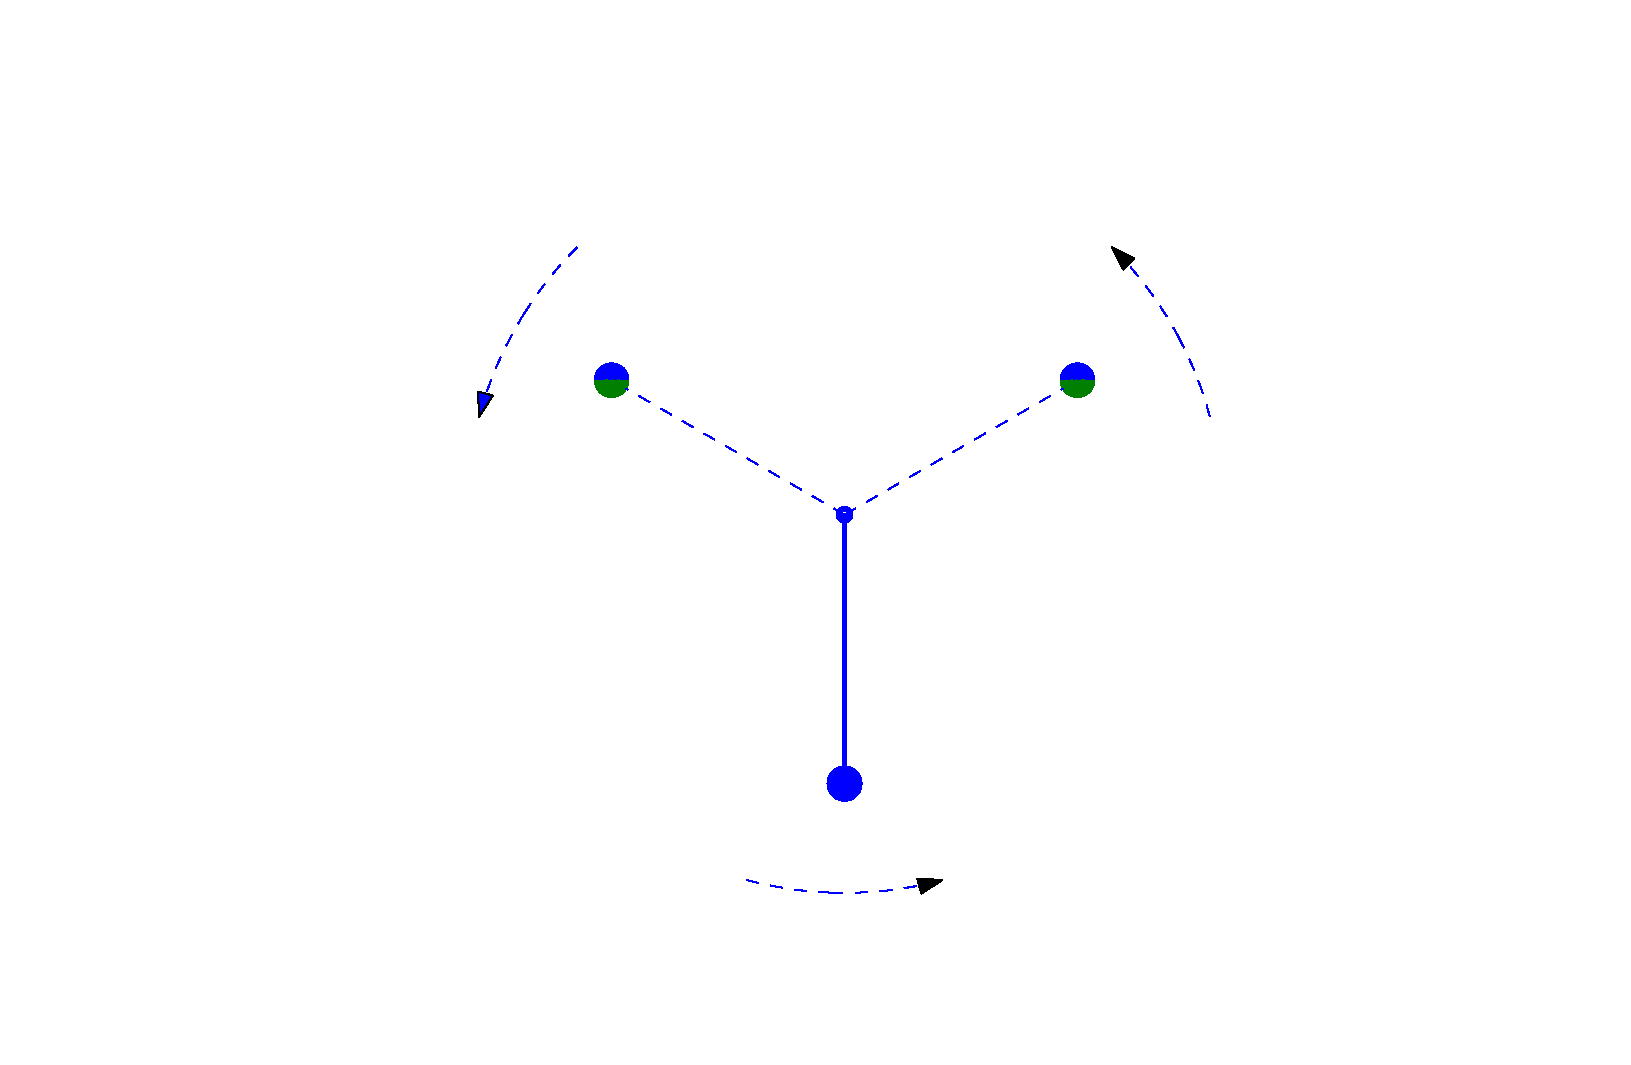
\includegraphics[bb=-78 148 689 643,width=5.67in,height=3.66in,keepaspectratio]{fig040408}}
\caption{The whirling undamped pendulum}
  \label{figure:4.4.8}
  \end{minipage}
  \hspace{0.5cm}
  \begin{minipage}[b]{0.5\linewidth}
    \centering
\scalebox{.7}{
  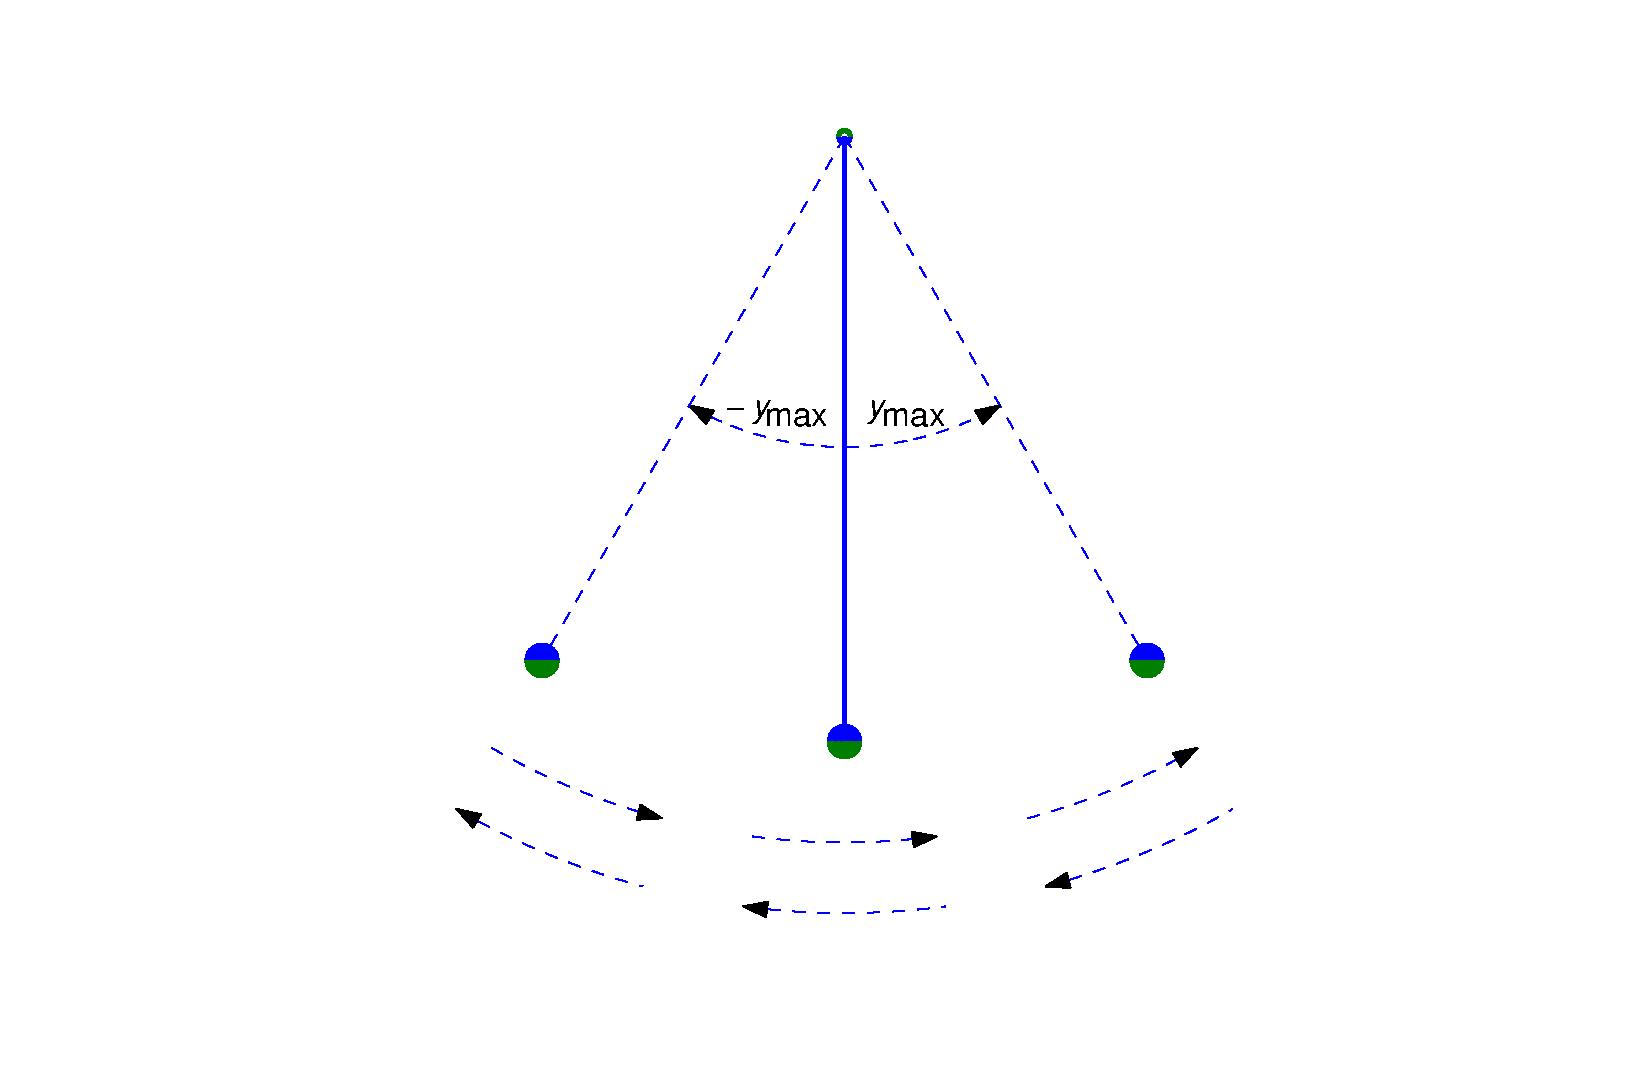
\includegraphics[bb=-78 148 689 643,width=5.67in,height=3.66in,keepaspectratio]{fig040409}}
\caption{ The oscillating undamped pendulum}
  \label{figure:4.4.9}
  \end{minipage}
\end{figure}

\boxit{Stability  and Instability Conditions for $y''+p(y)=0$}

\noindent
It can be shown (Exercise~\ref{exer:4.4.23}) that an equilibrium
$\overline y$ of an undamped equation
\begin{equation} \label{eq:4.4.18}
y''+p(y)=0
\end{equation}
is stable if there's an open interval $(a,b)$ containing $\overline
y$ such that
\begin{equation} \label{eq:4.4.19}
p(y)<0 \mbox{\; if \;}a<y<\overline y\mbox{\; and \;} p(y)>0 \mbox{\; if
\;}
\overline y<y<b.
\end{equation}
If we regard $p(y)$ as a force acting on a unit mass,
\eqref{eq:4.4.19} means that the force resists all sufficiently small
displacements from $\overline y$.

We've already seen examples illustrating this principle. The equation
\eqref{eq:4.4.9} for the undamped spring-mass system is of the form
\eqref{eq:4.4.18} with $p(y)=ky/m$, which has only the stable equilibrium
$\overline y=0$. In this case \eqref{eq:4.4.19} holds with $a=-\infty$ and
$b=\infty$. The equation \eqref{eq:4.4.13} for the undamped pendulum is of
the form \eqref{eq:4.4.18} with $p(y)=(g/L)\sin y$. We've seen that
$\overline y=2m\pi$ is a stable equilibrium if $m$ is an integer. In
this case
$$
p(y)=\sin y<0
\mbox{\; if \;}(2m-1)\pi<y<2m\pi
$$
and
$$
p(y)>0 \mbox{\; if \;}2m\pi<y<(2m+1)\pi.
$$

It can also be shown (Exercise~\ref{exer:4.4.24}) that $\overline y$ is
unstable if there's a $b>\overline y$ such that
\begin{equation} \label{eq:4.4.20}
p(y)<0\mbox{\; if \;}\overline y<y<b
\end{equation}
or an $a<\overline y$ such that
\begin{equation} \label{eq:4.4.21}
p(y)>0\mbox{\; if \;}a<y<\overline y.
\end{equation}
If we regard $p(y)$ as a force acting on a unit mass,
\eqref{eq:4.4.20} means that the force tends to increase all sufficiently
small positive displacements from $\overline y$, while \eqref{eq:4.4.21}
means that the force tends to increase the magnitude of all
sufficiently small negative displacements from $\overline y$.

The undamped pendulum also illustrates this principle. We've seen that
$\overline y=(2m+1)\pi$ is an unstable equilibrium if $m$ is an
integer. In this case
$$
\sin y<0\mbox{\; if \;}(2m+1)\pi<y<(2m+2)\pi,
$$
so \eqref{eq:4.4.20} holds with $b=(2m+2)\pi$, and
$$
\sin y>0\mbox{\; if \;}2m\pi<y<(2m+1)\pi,
$$
so \eqref{eq:4.4.21} holds with $a=2m\pi$.

\begin{example} \label{example:4.4.3}\rm
The equation
\begin{equation} \label{eq:4.4.22}
y''+y(y-1)=0
\end{equation}
is of the form \eqref{eq:4.4.18} with $p(y)=y(y-1)$. Therefore $\overline
y=0$ and $\overline y=1$ are the equilibria of \eqref{eq:4.4.22}. Since
\begin{eqnarray*}
y(y-1)>0 &\text{\, if \,} y<0\mbox{\, or \,}y>1,\\
<0&\hspace*{-22pt}\text{\, if \,} 0<y<1,
\end{eqnarray*}
$\overline y=0$ is unstable and $\overline y=1$ is
stable.

The phase plane equivalent of \eqref{eq:4.4.22} is the separable equation
$$
v{dv\over dy}+y(y-1)=0.
$$
Integrating yields
$$
{v^2\over2}+{y^3\over3}-{y^2\over2}=C,
$$
which we rewrite  as
\begin{equation} \label{eq:4.4.23}
v^2+{1\over3}y^2(2y-3)=c
\end{equation}
after renaming the constant of integration. These are the trajectories
of \eqref{eq:4.4.22}. If $y$ is any solution of \eqref{eq:4.4.22},  the
point $(y(t),v(t))$ moves along the trajectory of $y$ in the direction
of increasing $y$ in the upper half plane ($v=y'>0$), or in the
direction of decreasing $y$ in the lower half plane ($v=y'<0$).

Figure~\ref{figure:4.4.10}  shows
typical trajectories. The
dashed curve through the critical point $(0,0)$, obtained by setting
$c=0$ in \eqref{eq:4.4.23}, separates the $y$-$v$ plane into regions
that contain different kinds of trajectories; again,
 we call this curve a {\color{blue}\it separatrix\/}.
Trajectories in the region bounded by the closed loop \part{b} are closed
curves,
so solutions associated with them are periodic. Solutions associated
with other trajectories are not periodic. If $y$ is any such solution
with trajectory not  on the separatrix, then
$$
\begin{array}{llrllr}
\dst\lim_{t\to\infty}y(t)&=&-\infty, &\dst\lim_{t\to-\infty}y(t)&=&-\infty,\\
\dst\lim_{t\to\infty}v(t)&=&-\infty,
&\dst\lim_{t\to-\infty}v(t)&=&\infty.
\end{array}
$$

 \begin{figure}[H]
  \centering
  \color{blue}
  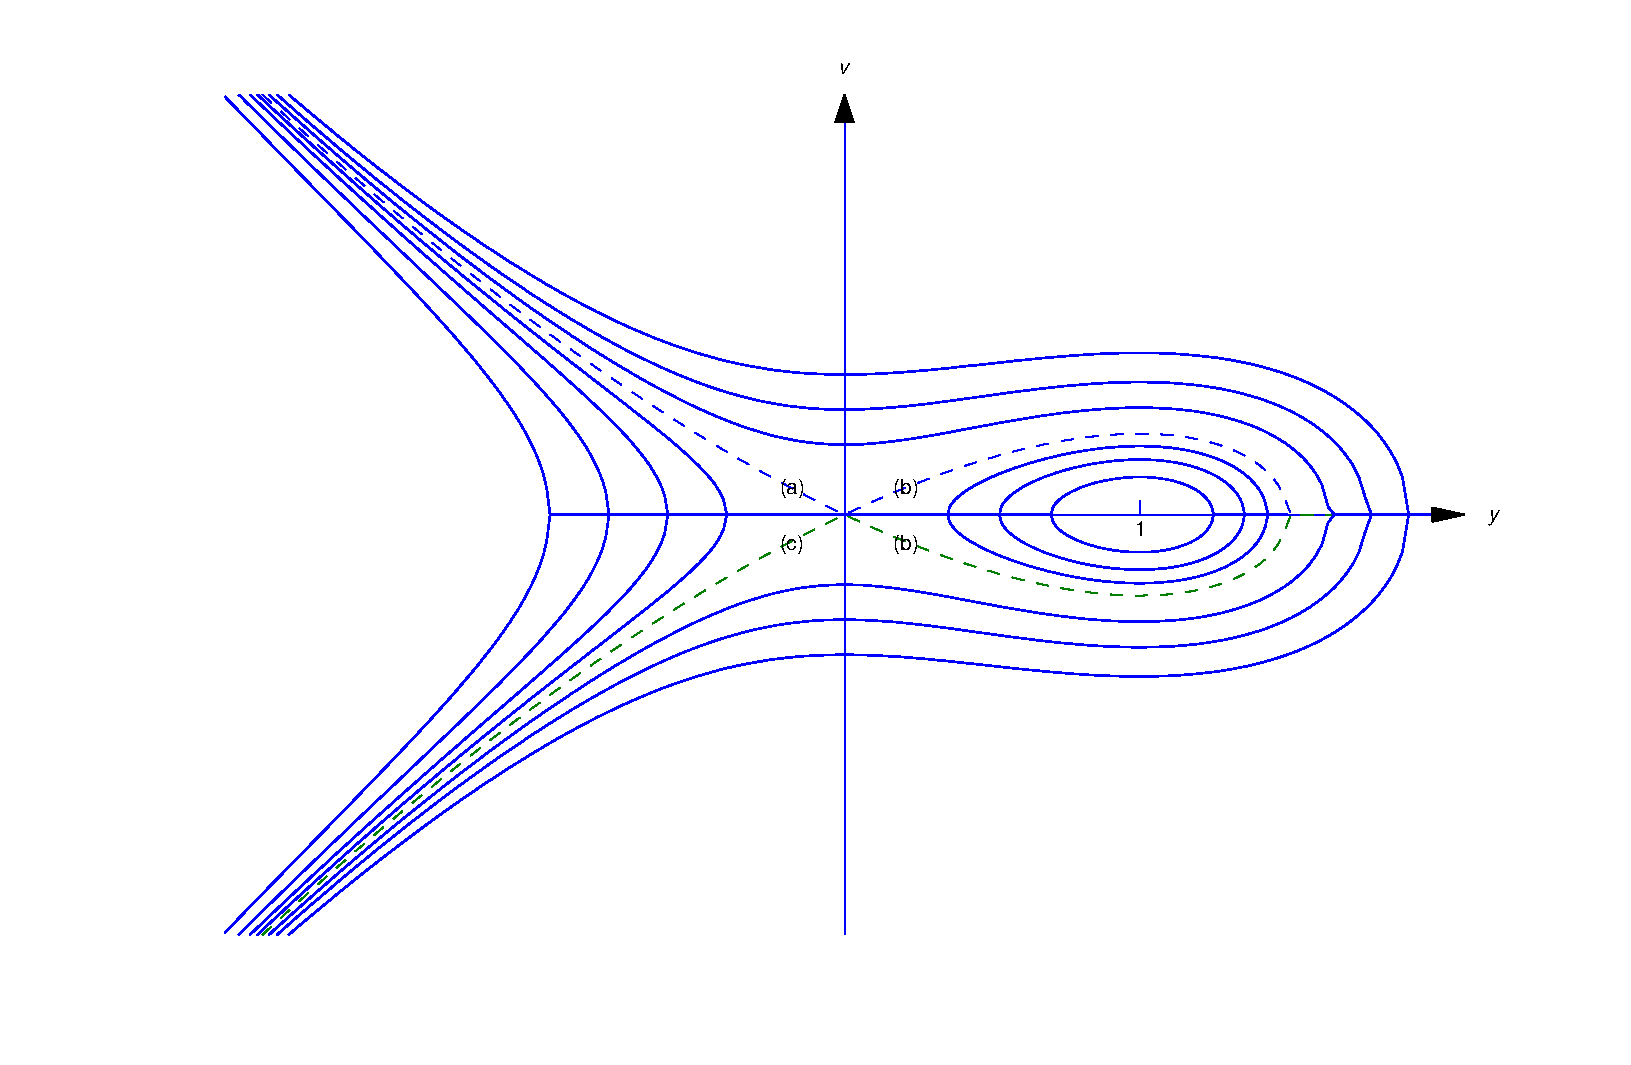
\includegraphics[bb=-78 148 689 643,width=5.67in,height=3.66in,keepaspectratio]{fig040410}
\caption{ Trajectories of $y''+y(y-1)=0$}
  \label{figure:4.4.10}
\end{figure}

The separatrix contains four trajectories of \eqref{eq:4.4.22}. One is the
point $(0,0)$, the trajectory of the equilibrium $\overline y=0$.
Since distinct trajectories can't intersect, the segments of the
separatrix marked \part{a}, \part{b}, and \part{c} -- which don't include $(0,0)$ --
are distinct trajectories, none of which can be traversed in finite
time. Solutions with these trajectories have the following asymptotic
behavior:
$$
\begin{array}{llrllrl}
\dst\lim_{t\to\infty}y(t)&=&0, &\dst\lim_{t\to-\infty}y(t)&=&-\infty,\\
\dst\lim_{t\to\infty}v(t)&=&0,
&\dst\lim_{t\to-\infty}v(t)&=&\infty\phantom{,}&
\mbox{ (on \part{a})}  \\
\dst\lim_{t\to\infty}y(t)&=&0, &\dst\lim_{t\to-\infty}y(t)&=&0,\\
\dst\lim_{t\to\infty}v(t)&=&0,
&\dst\lim_{t\to-\infty}v(t)&=&0\phantom{,}&
\mbox{ (on \part{b})}  \\
\dst\lim_{t\to\infty}y(t)&=&-\infty, &\dst\lim_{t\to-\infty}y(t)&=&0,\\
\dst\lim_{t\to\infty}v(t)&=&-\infty,
&\dst\lim_{t\to-\infty}v(t)&=&0\phantom{,}&
\mbox{ (on \part{c})}.
\end{array}.
$$
\end{example}

\boxit{The Damped Case}

\noindent
The phase plane equivalent of the damped autonomous equation
\begin{equation} \label{eq:4.4.24}
y''+q(y,y')y'+p(y)=0
\end{equation}
is
$$
v{dv\over dy}+q(y,v)v+p(y)=0.
$$
This equation isn't  separable, so we can't solve it for $v$ in terms
of
$y$,
as we did in the undamped case, and conservation of energy doesn't
hold. (For example, energy expended in overcoming friction is lost.)
However, we can study the qualitative behavior of its solutions by
rewriting it as
\begin{equation} \label{eq:4.4.25}
{dv\over dy}=-q(y,v)-{p(y)\over v}
\end{equation}
and considering the direction fields for this equation. In the
following examples we'll also be showing computer generated
trajectories of this equation, obtained by numerical methods. The
exercises call for similar computations. The methods discussed in
Chapter~3
 are not suitable for this
task, since  $p(y)/v$ in \eqref{eq:4.4.25} is undefined on the $y$ axis
of the Poincar\'e phase plane. Therefore we're forced to apply
numerical methods briefly discussed in Section~10.1 to the
system
\begin{eqnarray*}
y'&=&v\\
v'&=&-q(y,v)v-p(y),
\end{eqnarray*}
which is equivalent to \eqref{eq:4.4.24} in the sense defined in
Section~10.1. Fortunately, most differential equation software
packages  enable you to do this painlessly.

In the text we'll confine ourselves to the case where $q$
is constant, so \eqref{eq:4.4.24} and \eqref{eq:4.4.25}  reduce to
\begin{equation} \label{eq:4.4.26}
y''+cy'+p(y)=0
\end{equation}
and
$$
{dv\over dy}=-c-{p(y)\over v}.
$$
(We'll consider more general equations in the exercises.) The constant
$c$ is called the {\color{blue}\it damping constant\/}. In situations where
\eqref{eq:4.4.26} is the equation of motion of an object, $c$ is positive;
however, there are situations where  $c$ may be negative.

\boxit{The Damped Spring-Mass System}

\noindent
Earlier we considered
the spring - mass system under the assumption that the only forces
acting on the object were gravity and the spring's resistance to
changes in its length. Now we'll assume that some mechanism (for
example, friction in the spring or atmospheric resistance) opposes the
motion of the object with a force proportional to its velocity. In
Section~6.1 it will be shown that in this case Newton's
second law of motion implies that
\begin{equation} \label{eq:4.4.27}
my''+cy'+ky=0,
\end{equation}
where $c>0$ is the {\color{blue}\it damping constant\/}. Again, this
equation can
be solved easily by a method that we'll study in Section~5.2,
but that method isn't available here. Instead, we'll consider its
phase plane equivalent, which can be written in the form \eqref{eq:4.4.25}
as
\begin{equation} \label{eq:4.4.28}
{dv\over dy}=-{c\over m}-{ky\over mv}.
\end{equation}
(A minor note: the $c$ in \eqref{eq:4.4.26} actually corresponds to
$c/m$ in this equation.) Figure~\ref{figure:4.4.11} shows a
typical direction field for an equation of this form. Recalling that
motion along a trajectory must be in the direction of increasing $y$
in the upper half plane ($v>0$) and in the direction of decreasing $y$
in the lower half plane ($v<0$), you can infer that all trajectories
approach the origin in clockwise fashion. To confirm this,
Figure~\ref{figure:4.4.12} shows the same direction field with some
trajectories filled in. All the trajectories shown there correspond to
solutions of the initial value problem
$$
my''+cy'+ky=0,\quad y(0)=y_0,\quad y'(0)=v_0,
$$
where
$$
mv_0^2+ky_0^2=\rho\quad (\mbox{a positive constant});
$$
thus, if there were no damping ($c=0$),  all the solutions would
have the same dashed elliptic trajectory, shown in
Figure~\ref{figure:4.4.14}.

\begin{figure}[htbp]
\color{blue}
  \begin{minipage}[b]{0.5\linewidth}
    \centering
   \scalebox{.65}{
  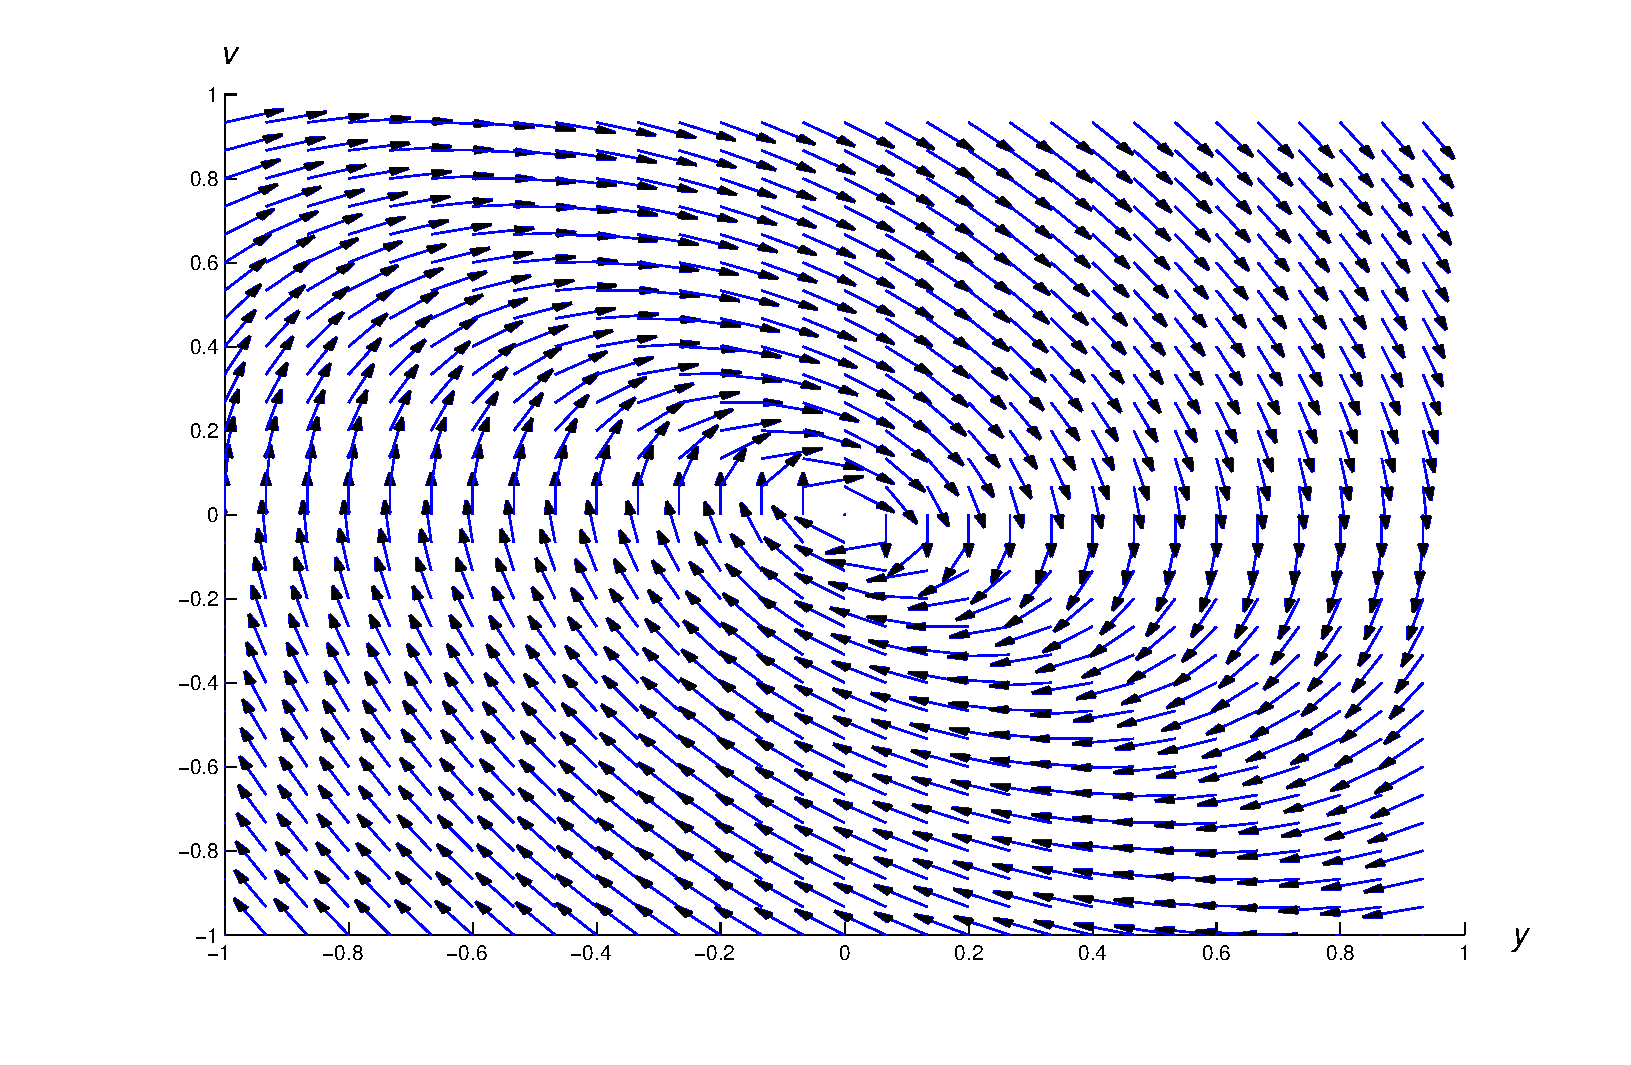
\includegraphics[bb=-78 148 689 643,width=5.67in,height=3.66in,keepaspectratio]{fig040411}}
\caption{ A typical direction field for
$my''+cy'+ky=0$ with $0<c<c_1$}
  \label{figure:4.4.11}
  \end{minipage}
  \hspace{0.6cm}
  \begin{minipage}[b]{0.5\linewidth}
    \centering
   \scalebox{.65}{
  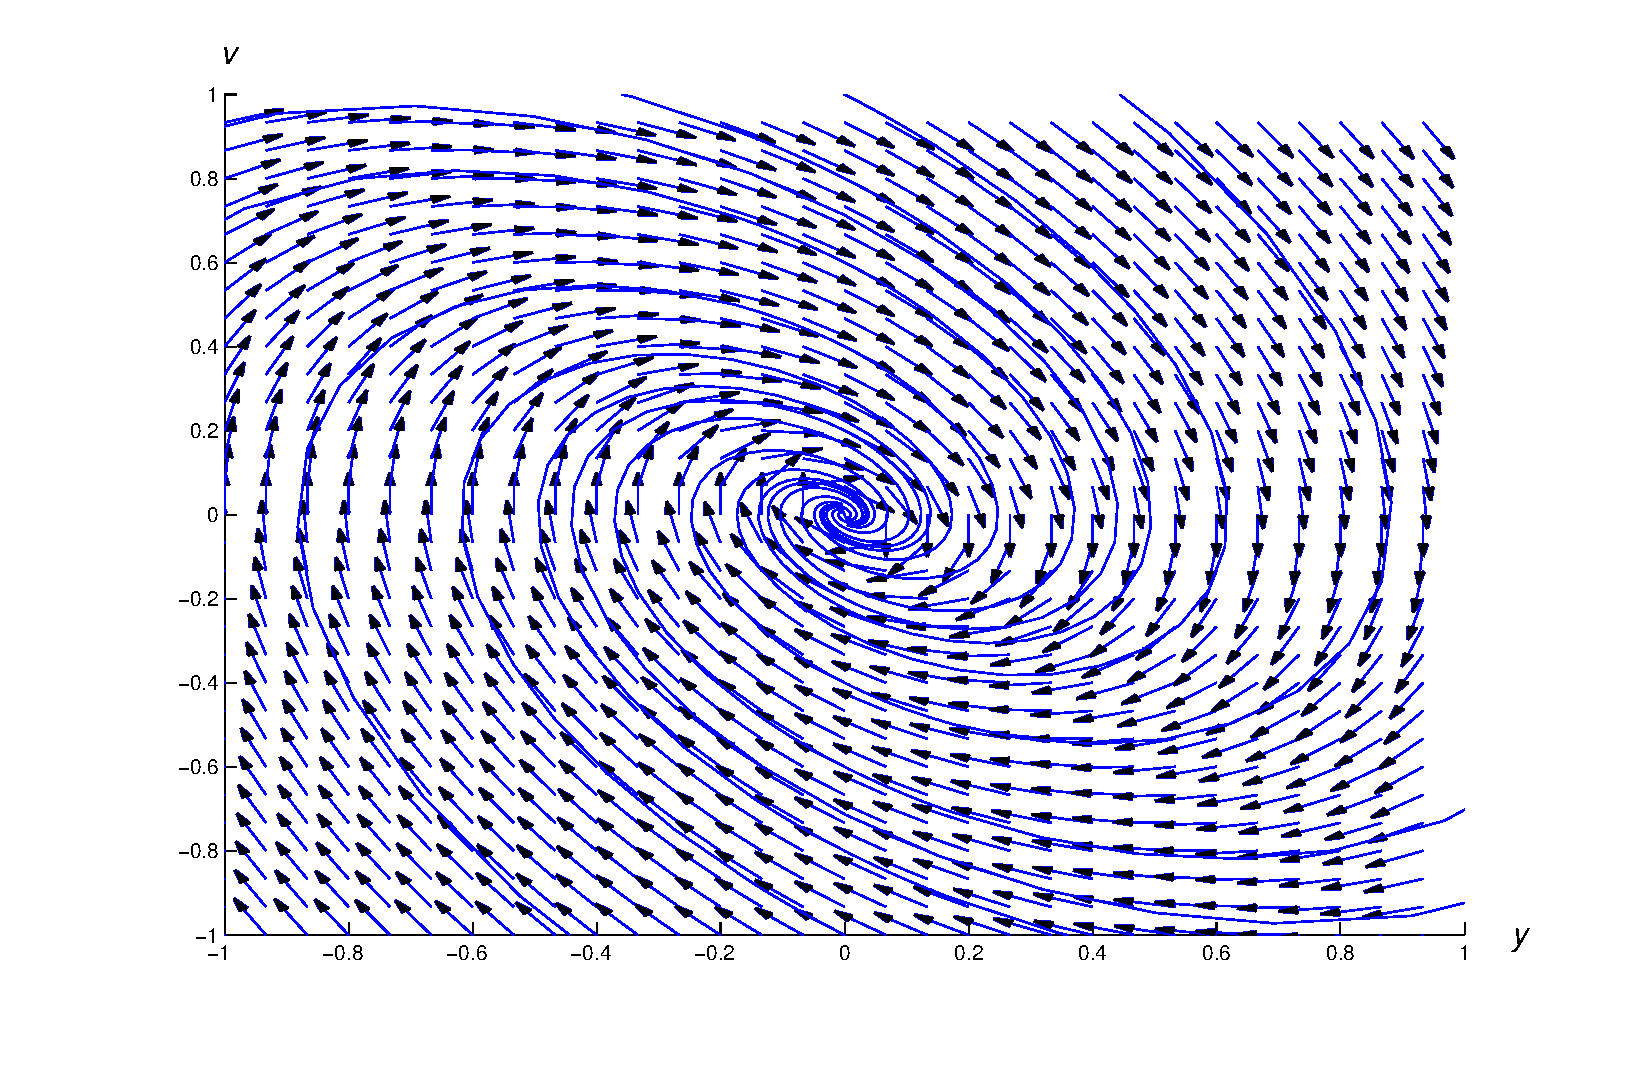
\includegraphics[bb=-78 148 689 643,width=5.67in,height=3.66in,keepaspectratio]{fig040412}}
\caption{ Figure~\ref{figure:4.4.11}
with some trajectories added}
  \label{figure:4.4.12}
  \end{minipage}
\end{figure}

Solutions corresponding to the trajectories in
Figure~\ref{figure:4.4.12} cross the $y$-axis infinitely many times.
The corresponding solutions are said to be {\color{blue}\it
oscillatory\/} (Figure~\ref{figure:4.4.13}) It is shown in
Section~6.2 that there's a number $c_1$ such that if $0\le
c<c_1$ then  all solutions of \eqref{eq:4.4.27} are oscillatory, while if
$c\ge c_1$,  no solutions of \eqref{eq:4.4.27} have this property. (In
fact, no solution not identically zero can have more than two zeros in
this case.) Figure~\ref{figure:4.4.14} shows a direction field and
some integral curves for \eqref{eq:4.4.28} in this case.

\begin{figure}[H]
  \centering
\scalebox{.7}{
  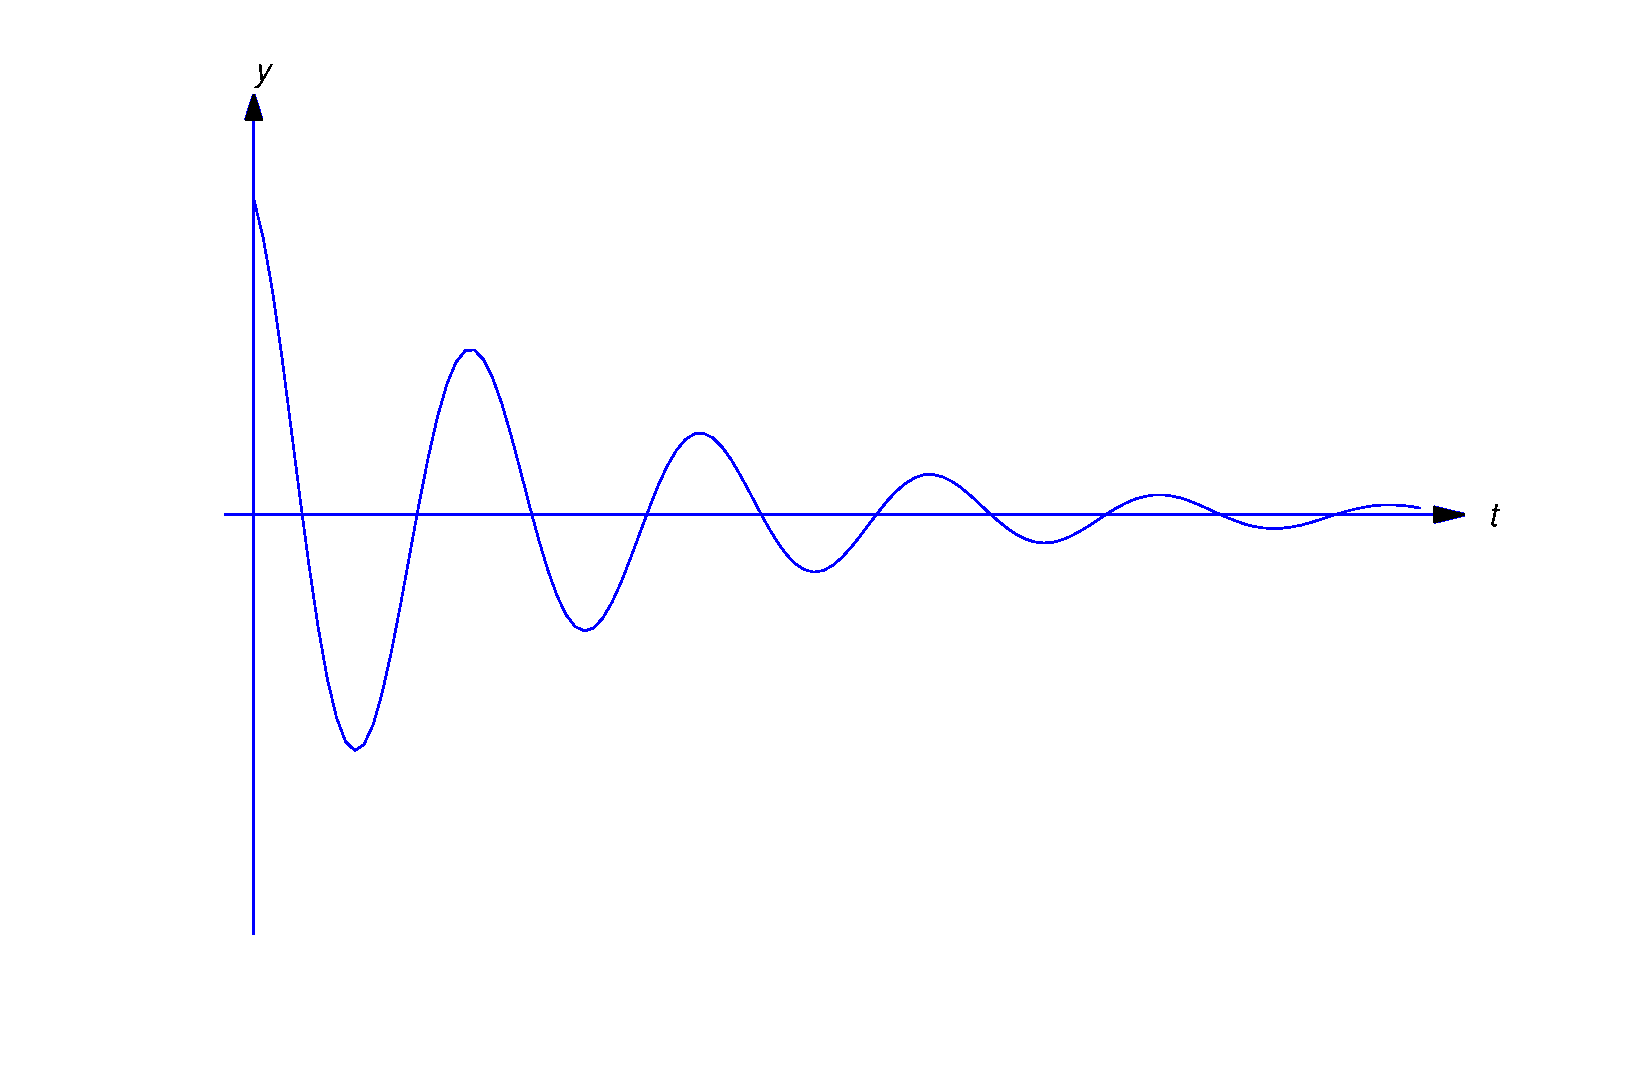
\includegraphics[bb=-78 148 689 643,width=5.67in,height=3.66in,keepaspectratio]{fig040413}}
\color{blue}
\caption{ An oscillatory solution of $my''+cy'+ky=0$}
  \label{figure:4.4.13}
\end{figure}

\begin{example}[The Damped Pendulum]\label{example:4.4.5} \rm
Now we
return to the pendulum. If we assume that
some mechanism (for example, friction in the axle or atmospheric
resistance) opposes the motion of the pendulum with a force
proportional to its angular velocity,  Newton's second law of
motion implies that
\begin{equation} \label{eq:4.4.29}
mLy''=-cy'-mg\sin y,
\end{equation}
where $c>0$ is the damping constant. (Again, a minor note: the $c$
in \eqref{eq:4.4.26} actually corresponds to $c/mL$ in this equation.)
To plot a direction field for \eqref{eq:4.4.29} we write its phase plane
equivalent as
$$
{dv\over dy}=-{c\over mL}-{g\over Lv}\sin y.
$$
Figure~\ref{figure:4.4.15} shows
trajectories of four solutions of \eqref{eq:4.4.29}, all satisfying
$y(0)=0$. For each $m=0$, $1$, $2$, $3$, imparting the initial velocity
$v(0)=v_m$ causes the pendulum to make $m$ complete revolutions and
then settle into decaying oscillation about the stable equilibrium
$\overline y=2m\pi$.
\end{example}

\begin{figure}[H]
  \centering
\scalebox{.8}{
  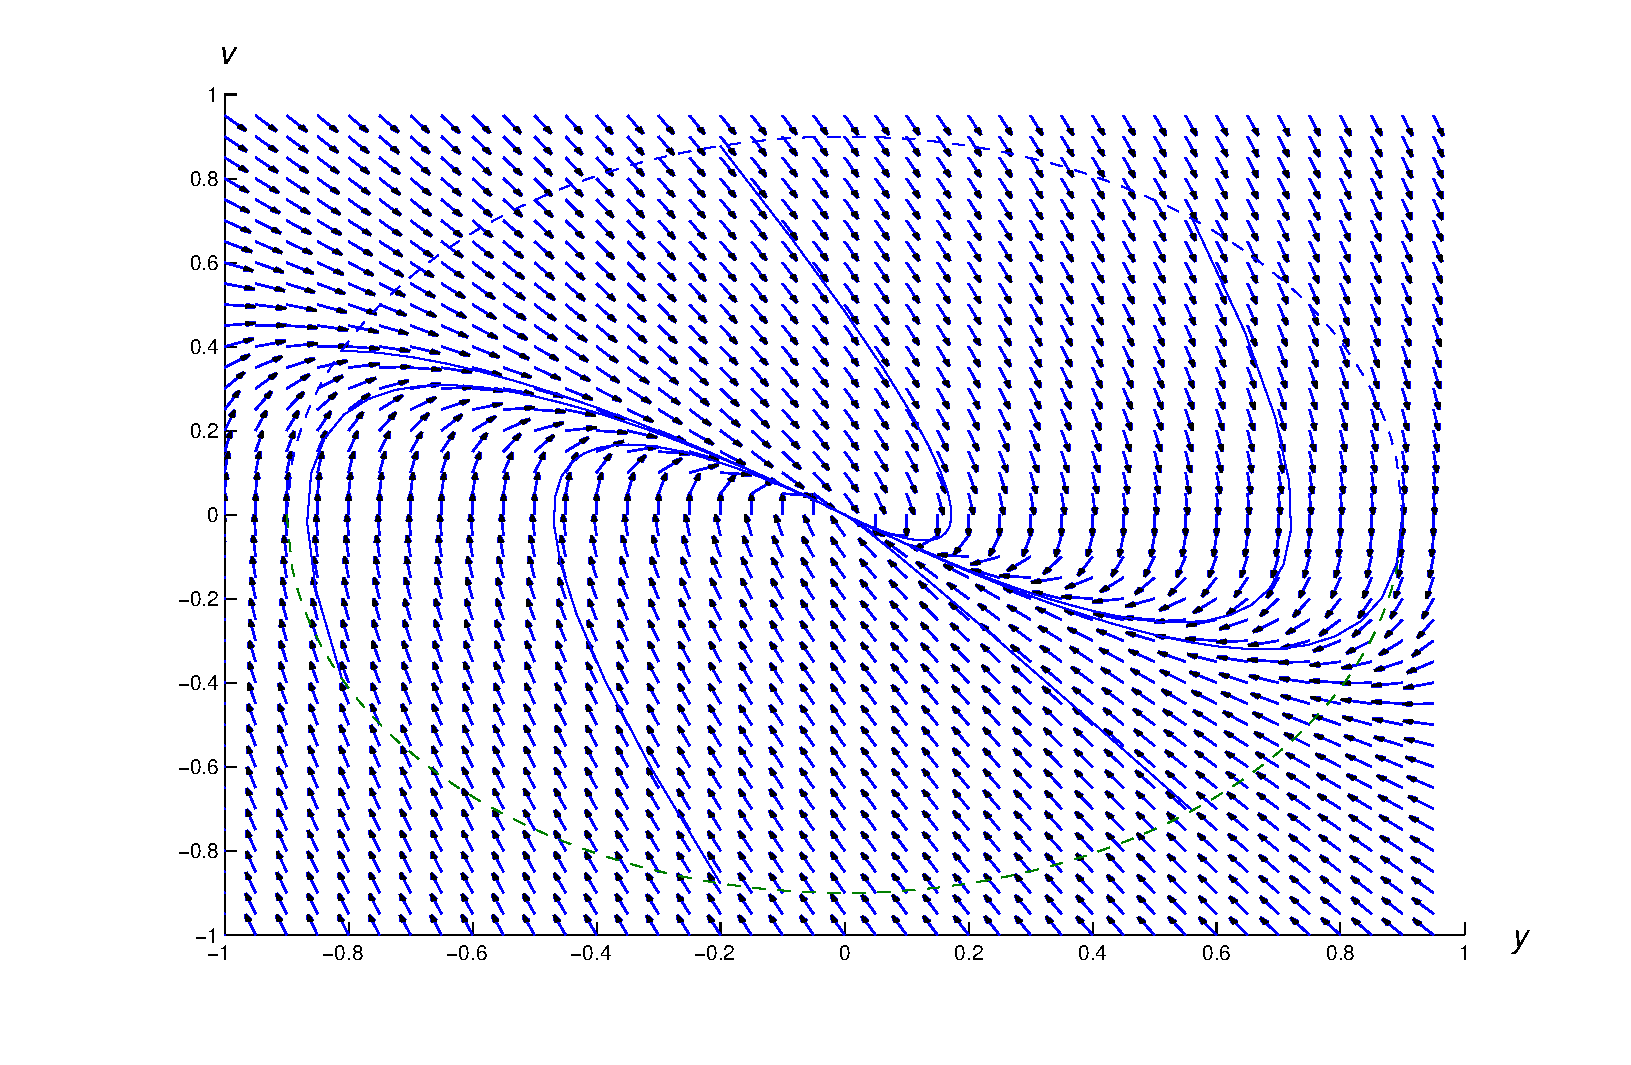
\includegraphics[bb=-78 148 689 643,width=5.67in,height=3.66in,keepaspectratio]{fig040414}}
\color{blue}
\caption{ A typical direction field for
$my''+cy'+ky=0$ with $c>c_1$}
  \label{figure:4.4.14}
\end{figure}

\begin{figure}[H]
  \centering
  \scalebox{.8}{
  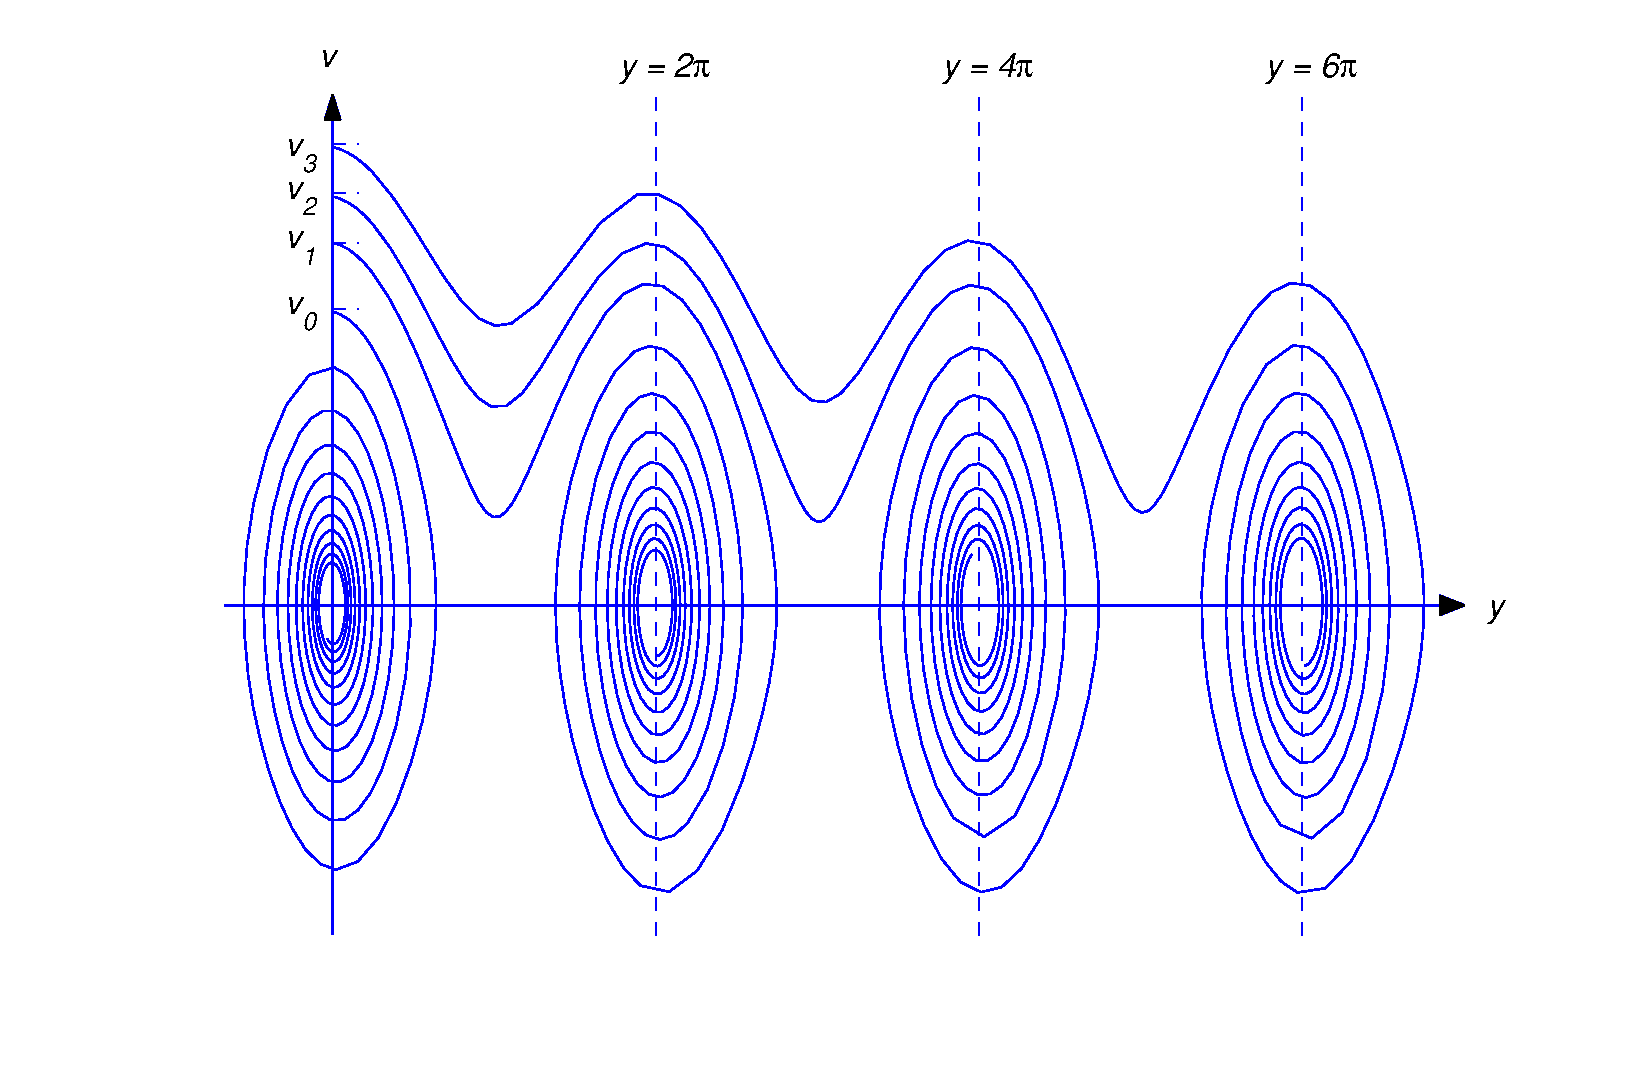
\includegraphics[bb=-78 148 689 643,width=5.67in,height=3.66in,keepaspectratio]{fig040415}}
\color{blue}
\caption{ Four  trajectories of the damped pendulum}
  \label{figure:4.4.15}
\end{figure}

\newpage

\exercises
In Exercises~\ref{exer:4.4.1}--\ref{exer:4.4.4} find the equations of the
trajectories of the given undamped equation. Identify the equilibrium
solutions, determine whether they are stable or unstable, and
plot some trajectories. \hint{Use Eqn.~\eqref{eq:4.4.8} to
obtain the equations of the trajectories.}

\begin{exerciselist}
\begin{tabular}[t]{@{}p{168pt}@{}p{168pt}}
\item\label{exer:4.4.1} \CGex $y''+y^3=0$ &
\vspace*{10pt}\item\label{exer:4.4.2} \CGex $y''+y^2=0$
\end{tabular}

\begin{tabular}[t]{@{}p{168pt}@{}p{168pt}}
\item\label{exer:4.4.3} \CGex$ y''+y|y|=0$ &
\item\label{exer:4.4.4} \CGex $y''+ye^{-y}=0$
\end{tabular}

\exercisetext{
In Exercises~\ref{exer:4.4.5}--\ref{exer:4.4.8} find the equations of the
trajectories of the given undamped equation. Identify the equilibrium
solutions,
determine whether they are stable or unstable, and find the equations
of the separatrices (that is, the curves through the unstable
equilibria). Plot the separatrices and some
trajectories in each of the regions of Poincar\'e plane determined by
them. \hint{Use Eqn.~\eqref{eq:4.4.17} to determine the separatrices.}}

\begin{tabular}[t]{@{}p{168pt}@{}p{168pt}}
\item\label{exer:4.4.5} \CGex $y''-y^3+4y=0$ &
\vspace*{10pt}\item\label{exer:4.4.6} \CGex $y''+y^3-4y=0$
\end{tabular}

%\begin{tabular}[t]{@{}p{168pt}@{}p{168pt}}
\begin{tabular}[t]{@{}p{178pt}@{}p{168pt}}
\item\label{exer:4.4.7} \CGex $y''+y(y^2-1)(y^2-4)=0$&
\item\label{exer:4.4.8} \CGex $y''+y(y-2)(y-1)(y+2)=0$
\end{tabular}

\exercisetext{In Exercises~\ref{exer:4.4.9}--\ref{exer:4.4.12}
plot some trajectories of the given equation for various values
(positive, negative, zero) of the parameter $a$. Find the equilibria
of the equation and classify them as stable or unstable. Explain why
the phase plane plots corresponding to positive and negative values of
$a$ differ so markedly. Can you think of a reason why zero deserves to
be called the {\color{blue}\it critical value\/} of $a$?}

\begin{tabular}[t]{@{}p{168pt}@{}p{168pt}}
\item\label{exer:4.4.9} \Lex $y''+y^2-a=0$&
\vspace*{10pt}\item\label{exer:4.4.10} \Lex $y''+y^3-ay=0$
\end{tabular}

\begin{tabular}[t]{@{}p{168pt}@{}p{168pt}}
\item\label{exer:4.4.11} \Lex $y''-y^3+ay=0$&
\item\label{exer:4.4.12} \Lex $y''+y-ay^3=0$
\end{tabular}
\exercisetext{In Exercises~\ref{exer:4.4.13}-\ref{exer:4.4.18}
plot trajectories of the given equation for $c=0$ and small nonzero
(positive and negative) values of $c$ to observe the effects of
damping.}

\begin{tabular}[t]{@{}p{168pt}@{}p{168pt}}
\item\label{exer:4.4.13} \Lex $y''+cy'+y^3=0$&
\vspace*{10pt}\item\label{exer:4.4.14} \Lex $y''+cy'-y=0$
\end{tabular}

\begin{tabular}[t]{@{}p{168pt}@{}p{168pt}}
\item\label{exer:4.4.15} \Lex $y''+cy'+y^3=0$&
\item\label{exer:4.4.16} \Lex $y''+cy'+y^2=0$
\end{tabular}

\begin{tabular}[t]{@{}p{168pt}@{}p{168pt}}
\item\label{exer:4.4.17} \Lex $y''+cy'+y|y|=0$&
\item\label{exer:4.4.18} \Lex $y''+y(y-1)+cy=0$
\end{tabular}

\item\label{exer:4.4.19} \Lex
The \href{https://mathshistory.st-andrews.ac.uk/Biographies/Van_der_Pol/}
{\color{blue}\it van der Pol equation}
$$
y''-\mu(1-y^2)y'+y=0,
\eqno{\rm(A)}
$$
where $\mu$ is a positive constant and $y$ is electrical current
(Section~6.3), arises in the study of an electrical circuit
whose resistive properties depend upon the current. The damping term \\
$-\mu(1-y^2)y'$ works to reduce $|y|$ if $|y|<1$ or to increase $|y|$
if
$|y|>1$. It can be shown that van der
Pol's equation has exactly one closed trajectory, which is called a
{\color{blue}\it limit cycle\/}. Trajectories inside the limit cycle spiral
outward to it, while trajectories outside the limit cycle spiral
inward to it (Figure~\ref{figure:4.4.16}). Use your favorite
differential equations software  to verify this for
$\mu=.5,1.1.5,2$. Use a grid with $-4<y<4$ and $-4<v<4$.

\begin{figure}[H]
  \centering
  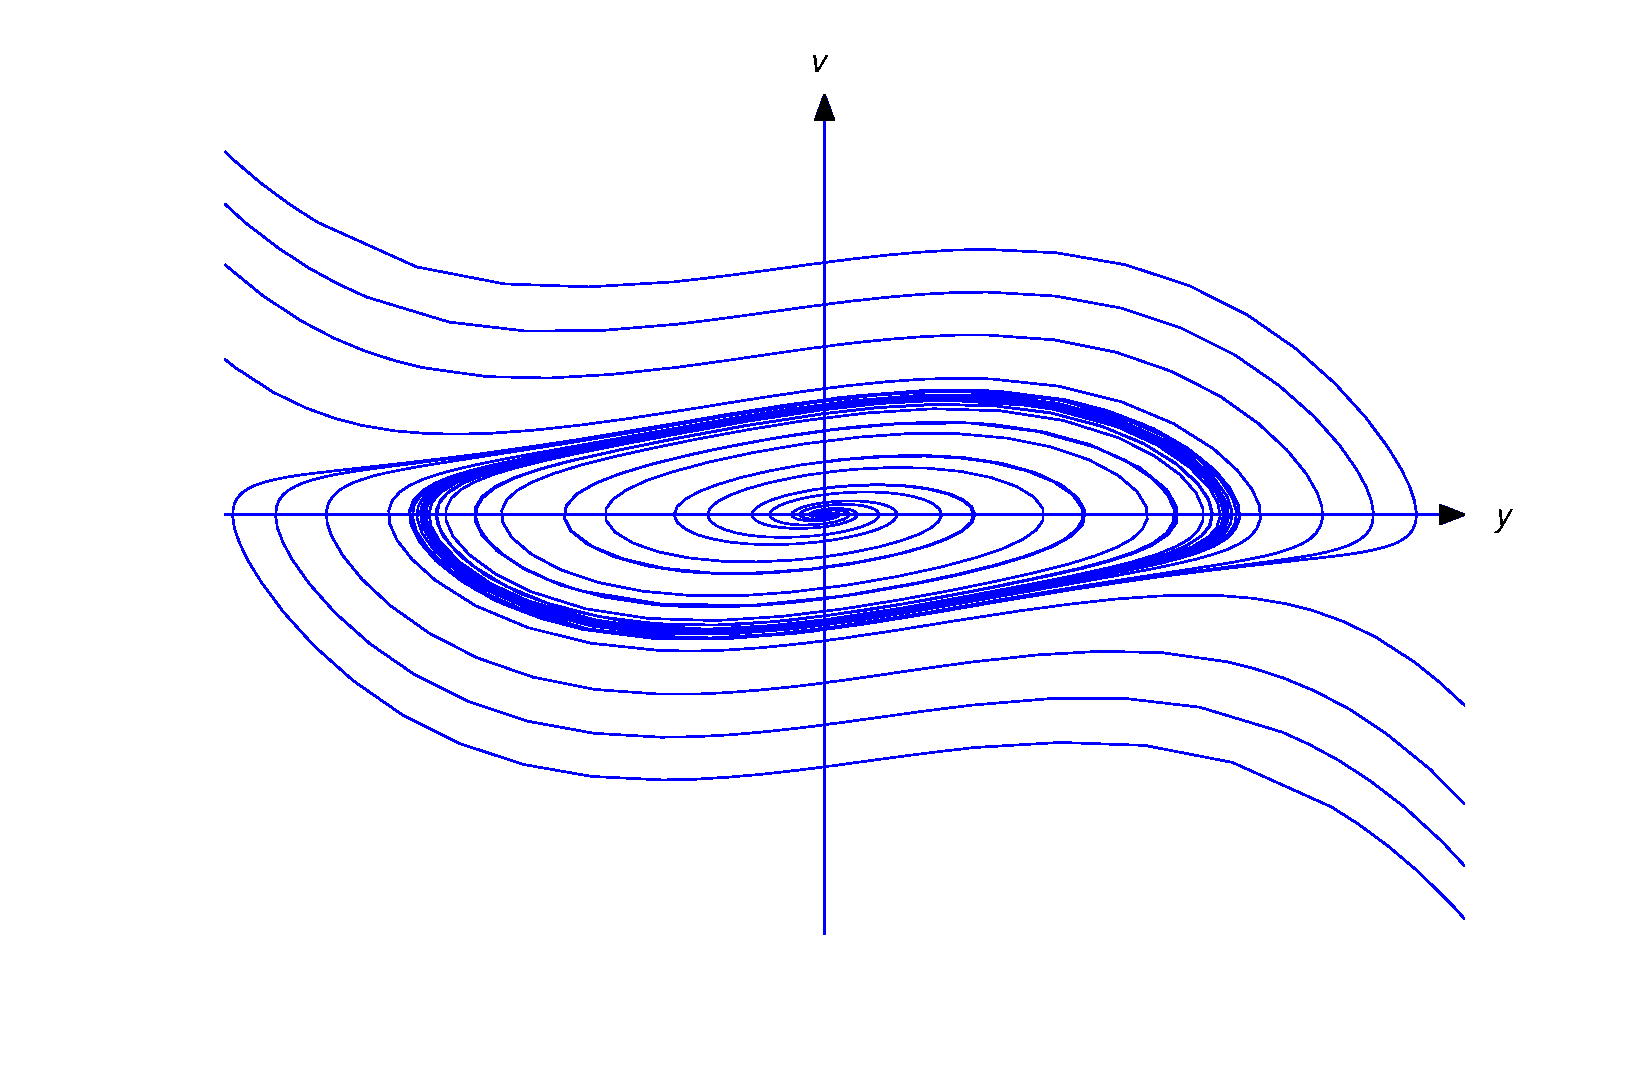
\includegraphics[bb=-78 148 689 643,width=5.67in,height=3.66in,keepaspectratio]{fig040416}
  \caption{Trajectories of van der Pol's equation}
  \label{figure:4.4.16}
\end{figure}

\item\label{exer:4.4.20}  \Lex
\href{https://mathshistory.st-andrews.ac.uk/Biographies/Rayleigh/}
{\color{blue}\it Rayleigh's equation},
$$
y''-\mu(1-(y')^2/3)y'+y=0
$$
also has a limit cycle. Follow the directions of
Exercise~\ref{exer:4.4.19} for this equation.

\item\label{exer:4.4.21}
In connection with Eqn~\eqref{eq:4.4.15},
suppose   $y(0)=0$ and $y'(0)=v_0$, where $0<v_0<v_c$.
\begin{alist}
\item % (a)
Let  $T_1$ be the time
required for  $y$ to increase from zero to
$y_{\max}=2\sin^{-1}(v_0/v_c)$. Show that
$$
{dy\over dt}=\sqrt{v_0^2-v_c^2\sin^2y/2},\quad 0\le t<T_1.
\eqno{\rm(A)}
$$
\item % (b)
Separate variables in (A) and show that
$$
T_1=\int_0^{y_{\max}}{du\over\sqrt{v_0^2-v_c^2\sin^2u/2}}
\eqno{\rm(B)}
$$
\item % (c)
Substitute $\sin u/2=(v_0/v_c)\sin\theta$ in (B) to obtain
$$
T_1=2\int_0^{\pi/2}{d\theta\over\sqrt{v_c^2-v_0^2\sin^2\theta}}.
\eqno{\rm(C)}
$$
\item % (d)
Conclude from  symmetry
that  the time required for  $(y(t),v(t))$ to traverse the
trajectory
$$
v^2=v_0^2-v_c^2\sin^2y/2
$$
is $T=4T_1$, and that consequently $y(t+T)=y(t)$ and $v(t+T)=v(t)$;
that is, the oscillation is periodic with period $T$.
\item % (e)
Show that if $v_0=v_c$,  the integral in (C) is improper and
diverges to $\infty$. Conclude from this  that $y(t)<\pi$
for all $t$ and $\lim_{t\to\infty}y(t)=\pi$.
\end{alist}

\item\label{exer:4.4.22}
Give a direct definition of an unstable equilibrium of $y''+p(y)=0$.

\item\label{exer:4.4.23}
Let $p$ be continuous for all $y$ and $p(0)=0$. Suppose there's
a positive number $\rho$ such that $p(y)>0$ if $0<y\le \rho$ and
$p(y)<0$ if $-\rho\le y<0$. For $0<r\le\rho$ let
$$
\alpha(r)=\min\left\{\int_0^r p(x)\,dx,\ \int_{-r}^0
|p(x)|\,dx\right\}
\mbox{\quad and \quad}
\beta(r)=\max\left\{\int_0^r p(x)\,dx,\ \int_{-r}^0
|p(x)|\,dx\right\}.
$$
Let $y$ be the solution of the initial value problem
$$
y''+p(y)=0,\quad y(0)=v_0,\quad y'(0)=v_0,
$$
and define
$c(y_0,v_0)=v_0^2+2\int_0^{y_0}p(x)\,dx$.
\begin{alist}
\item % (a)
Show that
$$
0<c(y_0,v_0) <v_0^2+2\beta(|y_0|)\mbox{\quad if \quad} 0<|y_0|\le\rho.
$$
\item % (b)
Show that
$$
v^2+2\int_0^y p(x)\,dx=c(y_0,v_0),\quad t>0.
$$
\item % (c)
Conclude from \part{b} that if $c(y_0,v_0)<2\alpha(r)$ then $|y|<r$, $t>0$.
\item % (d)
Given $\epsilon>0$, let  $\delta>0$ be chosen so that
$$
\delta^2+2\beta(\delta)<\max\left\{\epsilon^2/2,2\alpha(\epsilon/\sqrt2)
\right\}.
$$
Show that if $\sqrt{y_0^2+v_0^2}<\delta$ then
$\sqrt{y^2+v^2}<\epsilon$ for $t>0$, which implies that $\overline
  y=0$ is a stable equilibrium of $y''+p(y)=0$.
\item % (e)
Now let $p$
be continuous for all $y$ and $p(\overline y)=0$, where $\overline y$
is not necessarily zero. Suppose there's a positive number
$\rho$ such that $p(y)>0$ if $\overline y<y\le \overline y+\rho$ and
$p(y)<0$ if $\overline y-\rho\le y<\overline y$. Show that $\overline
y$ is a stable equilibrium of $y''+p(y)=0$.
\end{alist}

\item\label{exer:4.4.24}
Let $p$ be continuous for all $y$.
\begin{alist}
\item % (a)
Suppose $p(0)=0$ and there's a positive number $\rho$ such that
$p(y)<0$ if  $0<y\le \rho$. Let $\epsilon$ be any
number such that
$0<\epsilon<\rho$.
Show that if $y$ is the solution of the initial value problem
$$
y''+p(y)=0,\quad y(0)=y_0,\quad y'(0)=0
$$
with $0<y_0<\epsilon$, then
$y(t)\ge\epsilon$ for some
$t>0$. Conclude that $\overline y=0$ is an unstable equilibrium of
$y''+p(y)=0$. \hint{Let $k=\min_{y_0\le
x\le\epsilon}\left(-p(x)\right)$,
which is positive. Show that if $y(t)<\epsilon$ for $0\le t<T$ then
$kT^2<2(\epsilon-y_0)$.}
\item % (b)
Now let $p(\overline y)=0$, where $\overline y$ isn't  necessarily
zero. Suppose there's a positive number $\rho$ such that
$p(y)<0$ if $\overline y<y\le \overline y+\rho$. Show that $\overline
y$ is an unstable equilibrium of $y''+p(y)=0$.
\item % (c)
Modify your proofs of \part{a} and \part{b} to show that if there's a
positive
number $\rho$ such that $p(y)>0$ if $\overline y-\rho\le y<\overline
y$, then $\overline y$ is an unstable equilibrium of $y''+p(y)=0$.
\end{alist}

\end{exerciselist}


\section{Applications to Curves}

\noindent
\boxit{One-Parameter Families of Curves}

\noindent
We begin with two examples of families of curves generated by varying
a parameter over a set of real numbers.

\begin{example}\label{example:4.5.1} \rm
For each value of the parameter $c$, the equation
\begin{equation} \label{eq:4.5.1}
y-cx^2=0
\end{equation}
defines a curve in the $xy$-plane. If $c \ne0$, the curve is a
parabola through the origin, opening upward if $c>0$ or downward if
$c<0$.   If $c=0$, the curve is the $x$ axis (Figure~\ref{figure:4.5.1}).
\end{example}

\begin{figure}[H]
  \centering
  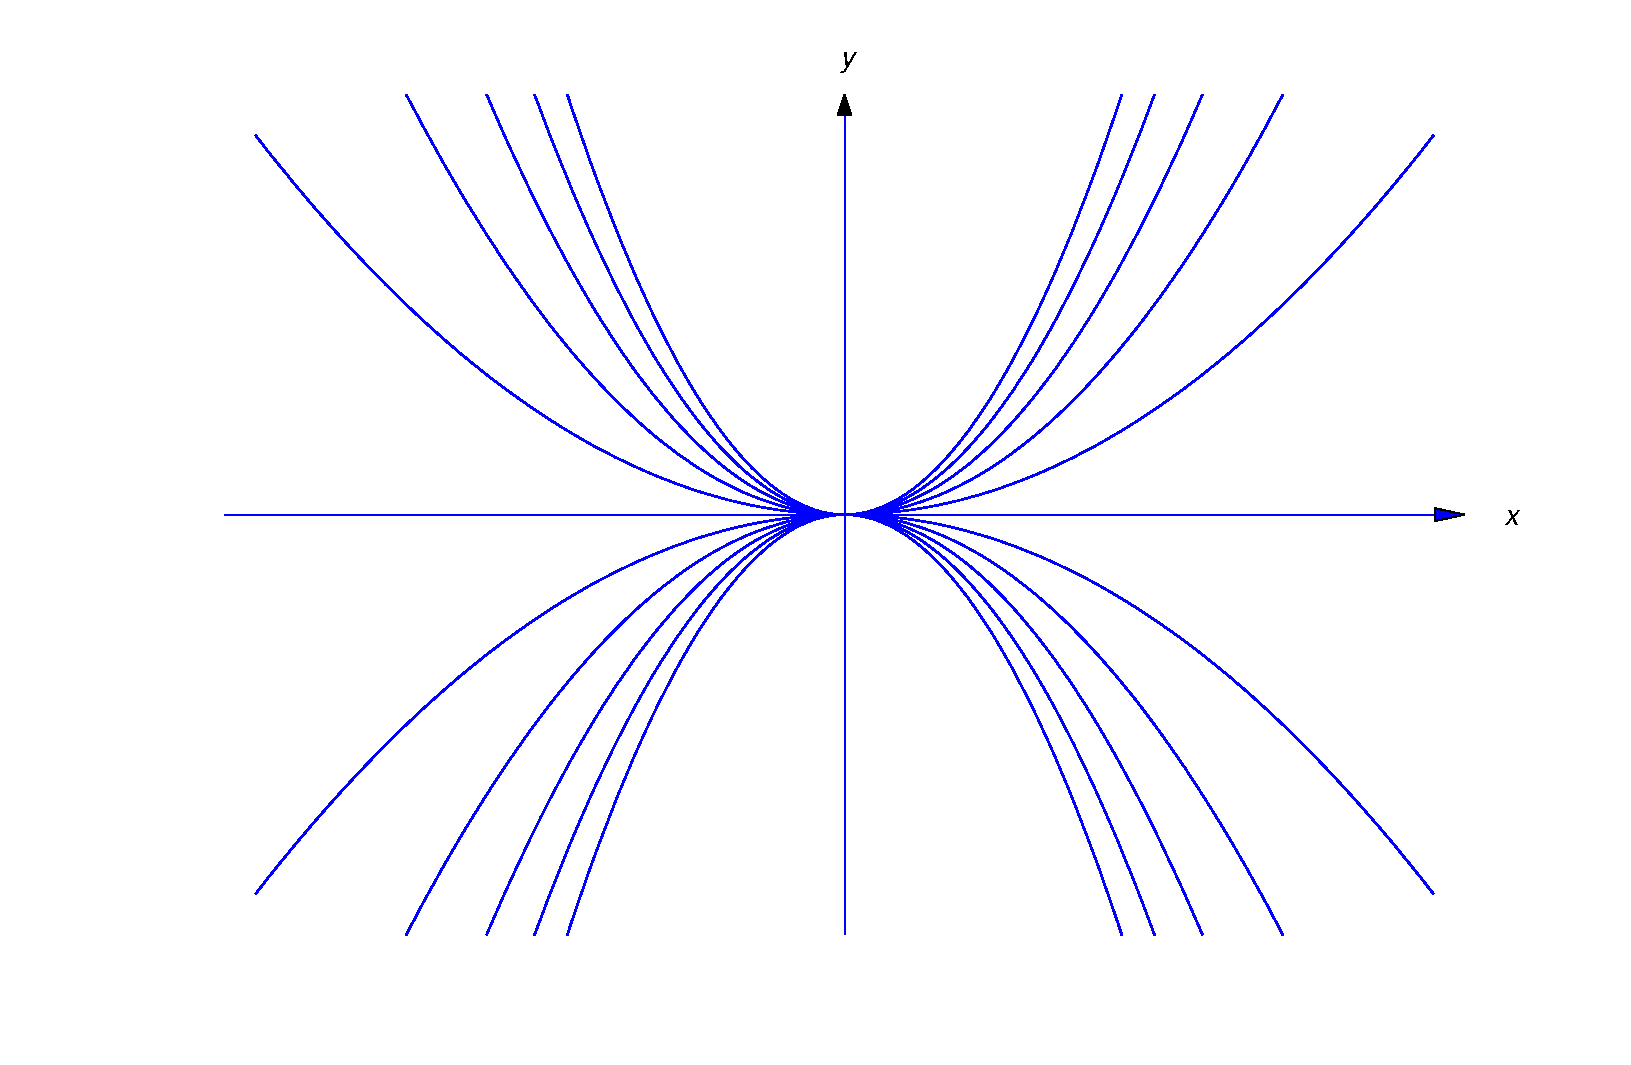
\includegraphics[bb=-78 148 689 643,width=5.67in,height=3.66in,keepaspectratio]{fig040501}
\color{blue}
  \caption{ A family of curves defined by $y-cx^2=0$}
  \label{figure:4.5.1}
\end{figure}

\begin{example} \label{example:4.5.2} \rm
For each value of the parameter $c$ the equation
\begin{equation} \label{eq:4.5.2}
y=x+c
\end{equation}
 defines a line with slope 1(Figure~\ref{figure:4.5.2}).
\end{example}

\begin{figure}[htbp]
\color{blue}
  \begin{minipage}[b]{0.5\linewidth}
    \centering
   \scalebox{.65}{
  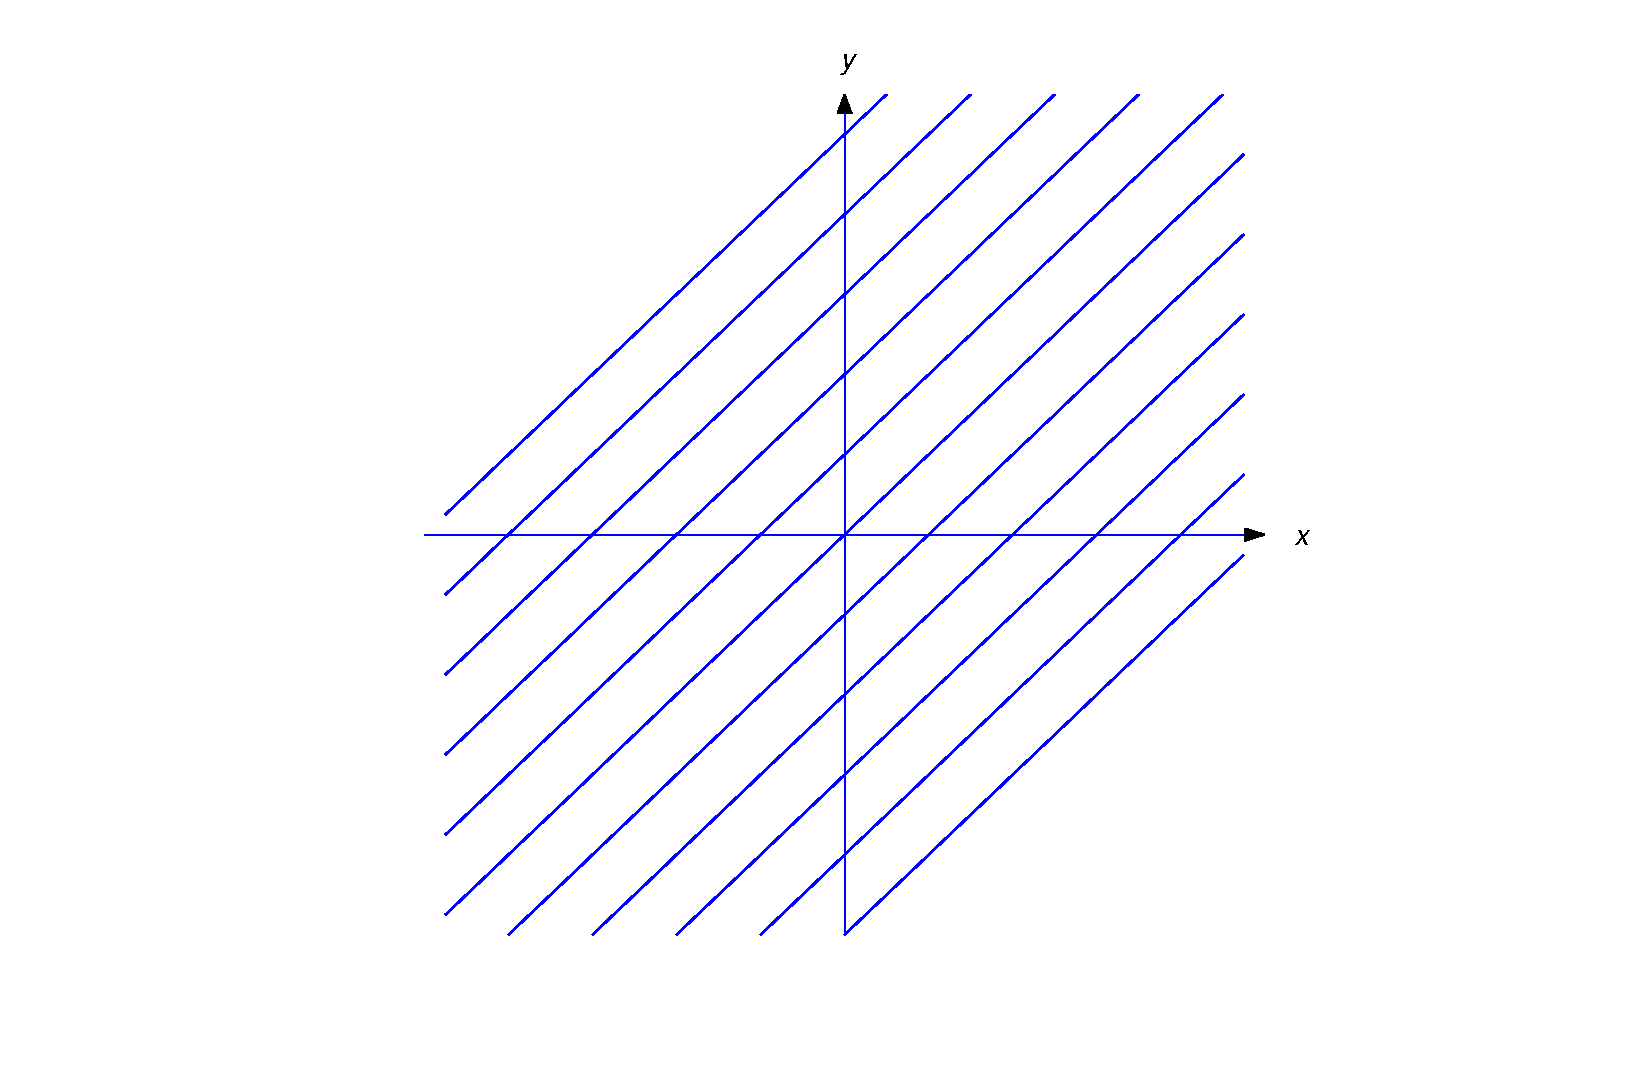
\includegraphics[bb=-78 148 689 643,width=5.67in,height=3.66in,keepaspectratio]{fig040502}}
  \caption{ A family of lines defined by $y=x+c$}
  \label{figure:4.5.2}
  \end{minipage}
  \hspace{0.6cm}
  \begin{minipage}[b]{0.5\linewidth}
    \centering
   \scalebox{.65}{
  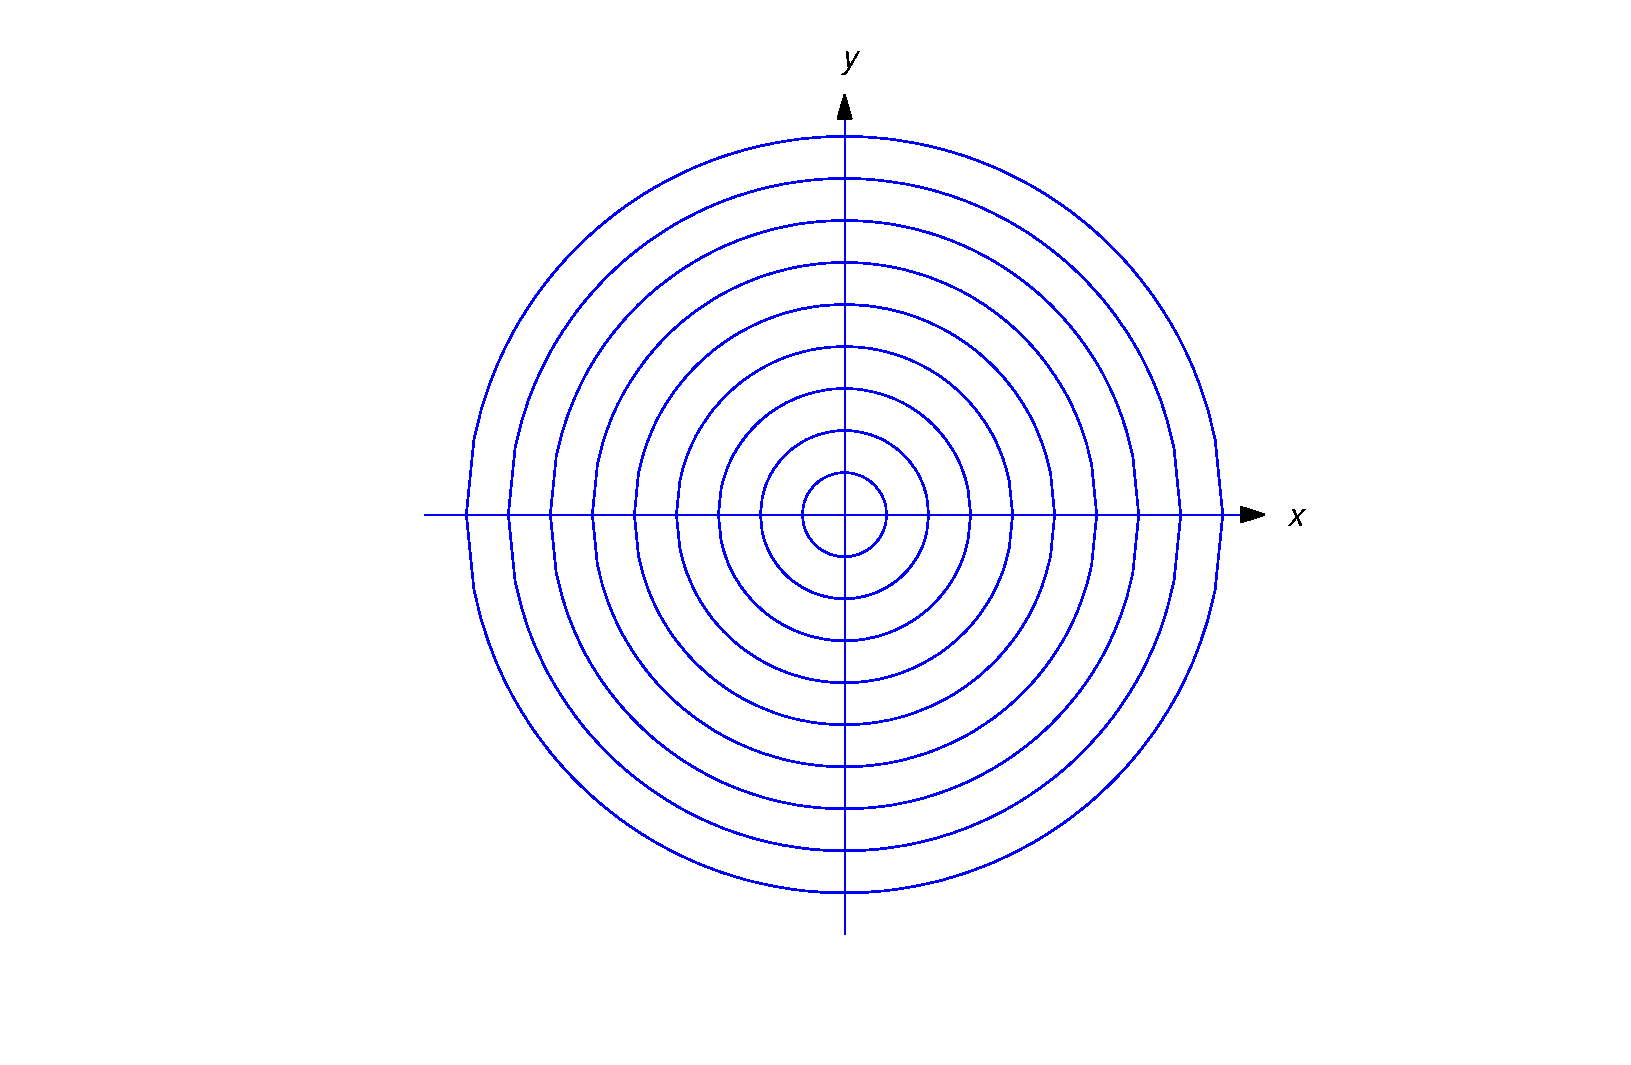
\includegraphics[bb=-78 148 689 643,width=5.67in,height=3.66in,keepaspectratio]{fig040503}}
  \caption{ A family of circles defined by $x^2+y^2-c^{2}=0$}
  \label{figure:4.5.3}
  \end{minipage}
\end{figure}

\begin{definition}\color{blue} \label{thmtype:4.5.1}
\rm An equation that can be written in the form
 \begin{equation} \label{eq:4.5.3}
H(x,y,c)=0
\end{equation}
is said to define a {\color{blue}\it one-parameter family of curves\/} if, for
each value of $c$ in some nonempty set of real numbers, the set of
points $(x,y)$ that satisfy  \eqref{eq:4.5.3} forms a curve in the
$xy$-plane.
\end{definition}

Equations \eqref{eq:4.5.1} and \eqref{eq:4.5.2} define one--parameter families
of curves. (Although \eqref{eq:4.5.2} isn't  in the form \eqref{eq:4.5.3}, it
can be written in this form as $y-x-c=0$.)

\begin{example}\label{example:4.5.3} \rm
If $c>0$,  the graph of the equation
\begin{equation} \label{eq:4.5.4}
x^2+y^2-c=0
\end{equation}
is a circle with center at $(0,0)$ and radius $\sqrt{c}$. If $c=0$, the
graph is the single point $(0,0)$. (We don't regard a single point as
a curve.) If $c<0$, the equation has no graph. Hence, \eqref{eq:4.5.4}
defines a one--parameter family of curves for positive values of $c$.
This family consists of all circles centered at $(0,0)$
(Figure~\ref{figure:4.5.3}).
\end{example}

\begin{example}\label{example:4.5.4} \rm
 The equation
$$
x^2+y^2+c^2=0
$$
does not define a one-parameter family of curves, since no $(x,y)$
satisfies the equation if $c\ne0$, and only the single point $(0,0)$
satisfies it if $c=0$. \bbox
\end{example}

Recall from Section~1.2 that the graph of a solution of a
differential equation is called an {\color{blue}\it integral curve\/} of the
equation. Solving a first order differential equation usually produces
a one--parameter family of integral curves of the equation. Here we
are interested in the converse problem:
given a one--parameter family of curves, is there a first order
differential equation for which every  member of the family is an integral
curve.
This suggests the next definition.

\begin{definition}\color{blue} \label{thmtype:4.5.2}
\rm If every curve in a one-parameter family defined by the equation
\begin{equation} \label{eq:4.5.5}
H(x,y,c)=0
\end{equation}
is an integral curve of the first order differential equation
\begin{equation} \label{eq:4.5.6}
F(x,y,y')=0,
\end{equation}
then  \eqref{eq:4.5.6} is said to be a {\color{blue}\it differential equation
for the family.\/}
\end{definition}

To find a differential equation for a one--parameter family we
differentiate its defining equation \eqref{eq:4.5.5} implicitly with
respect to $x$, to obtain
\begin{equation} \label{eq:4.5.7}
H_x(x,y,c)+H_y(x,y,c)y'=0.
\end{equation}
If this equation doesn't, then it's a differential
equation for the family. If it does contain $c$, it may be
possible to obtain a differential equation for the family by
eliminating $c$ between \eqref{eq:4.5.5} and \eqref{eq:4.5.7}.

\begin{example}\label{example:4.5.5}  \rm
Find a differential equation for the family of curves defined by
\begin{equation}  \label{eq:4.5.8}
y=cx^2.
\end{equation}
\end{example}

\solution Differentiating
\eqref{eq:4.5.8} with respect to $x$ yields
$$
y'=2cx.
$$
 Therefore $c=y'/2x$, and substituting this into
\eqref{eq:4.5.8} yields
$$
y={xy'\over2}
$$
 as a differential equation for the family of
curves defined by \eqref{eq:4.5.8}.  The graph of any function of
the form $y=cx^2$ is an integral curve of this equation. \bbox

The next example shows that members of a given family of curves
may be obtained by joining  integral curves for more than one
differential equation.

\begin{example}\label{example:4.5.6} \rm
\mbox{}
\begin{alist}
\item %(a)
Try to find a differential equation for the family of lines tangent
to the parabola $y=x^2$.

\item %(b)
Find two tangent lines to  the parabola $y=x^2$ that pass
through $(2,3)$, and find the points of tangency.
\end{alist}
\end{example}

\solutionpart{a} The equation of the line through a given point
$(x_0,y_0)$ with slope $m$ is
\begin{equation}  \label{eq:4.5.9}
y=y_0+m(x-x_0).
\end{equation}
If $(x_0,y_0)$ is on the parabola, then $y_0=x_0^2$ and the slope of
the tangent line through ($x_0,x_0^2)$ is $m=2x_0$; hence,
\eqref{eq:4.5.9} becomes
$$
y=x_0^2+2x_0(x-x_0),
$$
 or, equivalently,
\begin{equation} \label{eq:4.5.10}
y=-x_0^2+2x_0x.
\end{equation}
Here $x_0$ plays the role of the constant $c$ in
Definition~\ref{thmtype:4.5.1}; that is, varying $x_0$ over
$(-\infty,\infty)$ produces the family of tangent lines to the
parabola $y=x^2$.

Differentiating \eqref{eq:4.5.10} with respect to $x$ yields
$y'=2x_0$..
We can express $x_0$ in terms of $x$ and $y$ by rewriting
\eqref{eq:4.5.10} as
$$
x_0^2-2x_0x+y=0
$$
and using the quadratic formula to obtain
 \begin{equation}\label{eq:4.5.11}
 x_0=x\pm\sqrt{x^2-y}.
\end{equation}
We must choose the plus sign in \eqref{eq:4.5.11} if $x<x_0$
and the minus sign if $x>x_0$;   thus,
$$
x_0=\left(x+\sqrt{x^2-y}\right)\mbox{\, if \,} x<x_0
$$
 and
$$
x_0=\left(x-\sqrt{x^2-y}\right)\mbox{\, if \,} x>x_0.
$$
Since $y'=2x_0$, this implies that
\begin{equation} \label{eq:4.5.12}
y'=2\left(x+\sqrt{x^2-y}\right),\mbox{\quad if \quad} x<x_0
\end{equation}
 and
\begin{equation} \label{eq:4.5.13}
y'=2\left(x-\sqrt{x^2-y}\right),\mbox{\quad if \quad}x>x_0.
\end{equation}
Neither \eqref{eq:4.5.12} nor \eqref{eq:4.5.13} is a differential equation for
the family of tangent lines to the parabola $y=x^2$. However, if each
tangent line is regarded as consisting of two {\color{blue}\it tangent half
lines\/} joined at the point of tangency,   \eqref{eq:4.5.12} is a
differential equation for the family of tangent half lines on which
$x$ is less than the abscissa of the point of tangency
(Figure~\ref{figure:4.5.4}\part{a}), while \eqref{eq:4.5.13} is a
differential
equation for the family of tangent half lines on which $x$ is greater
than this abscissa (Figure~\ref{figure:4.5.4}(b)). The
parabola $y=x^2$ is also an integral curve of both \eqref{eq:4.5.12} and
\eqref{eq:4.5.13}.

\begin{figure}[H]
  \centering
  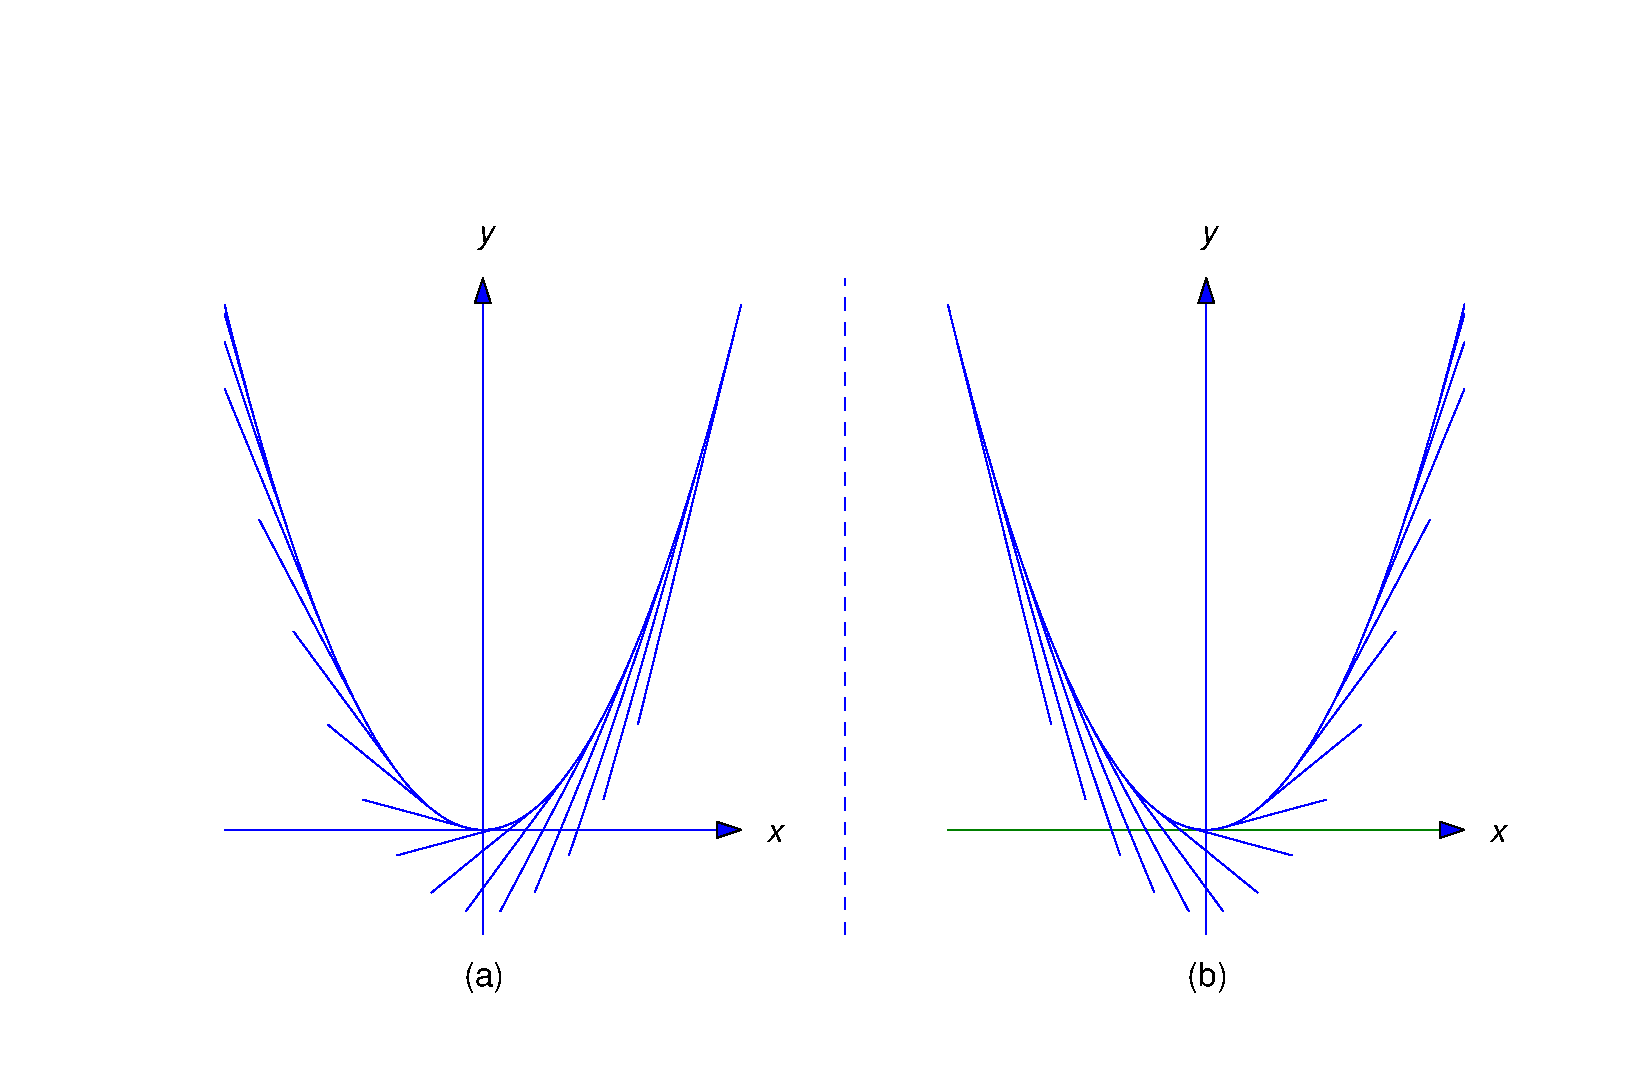
\includegraphics[bb=-78 148 689 643,width=5.67in,height=3.66in,keepaspectratio]{fig040504}
\color{blue}
  \caption{}
  \label{figure:4.5.4}
\end{figure}

\solutionpart{b}
From \eqref{eq:4.5.10} the point $(x,y)=(2,3)$ is on the tangent line
through $(x_0,x_0^2)$ if and only if
$$
3=-x_0^2+4x_0,
$$
which is equivalent to
$$
x_0^2-4x_0+3=(x_0-3)(x_0-1)=0.
$$
Letting $x_0=3$ in \eqref{eq:4.5.10} shows that $(2,3)$ is on the line
$$
y=-9+6x,
$$
which is tangent to the parabola at $(x_0,x_0^2)=(3,9)$, as shown in
Figure~\ref{figure:4.5.5}

Letting $x_0=1$ in \eqref{eq:4.5.10} shows that $(2,3)$ is on the line
$$
y=-1+2x,
$$
which is tangent to the parabola at $(x_0,x_0^2)=(1,1)$, as shown in
Figure~\ref{figure:4.5.5}.

 \vspace*{-15pt}
\begin{figure}[H]
  \centering
  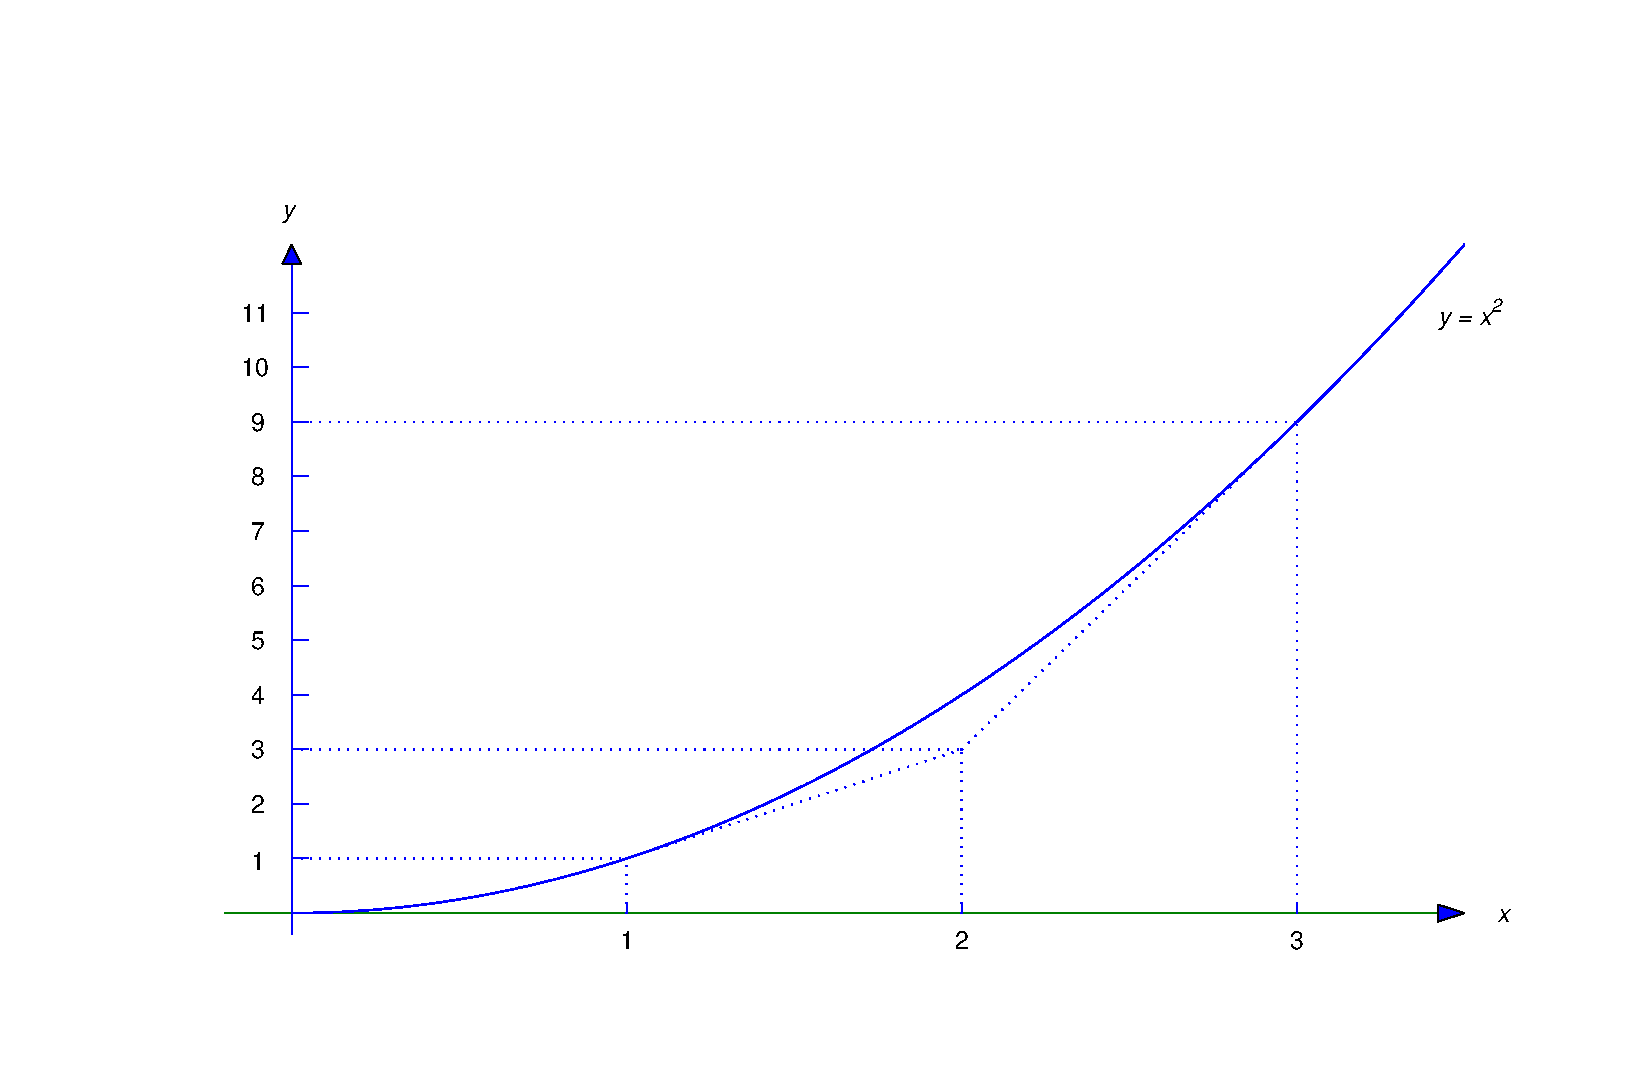
\includegraphics[bb=-78 148 689 643,width=5.67in,height=3.66in,keepaspectratio]{fig040505}
  \caption{}
  \label{figure:4.5.5}
\end{figure}

\boxit{Geometric Problems}

\noindent
We now consider some geometric problems that can be solved by means of
differential equations.

\begin{example}\label{example:4.5.7}   \rm
Find curves $y=y(x)$ such that every point $(x_0,y(x_0))$ on the curve
is the midpoint of the line segment with endpoints on the coordinate
axes and tangent to the curve at $(x_0,y(x_0))$
(Figure~\ref{figure:4.5.6}).
\end{example}

\solution
 The equation of the  line tangent to the curve at $P=(x_0,y(x_0)$ is
$$
y=y(x_0)+y'(x_0)(x-x_0).
$$
If we denote the $x$ and $y$ intercepts of the tangent line by $x_I$
and $y_I$ (Figure~\ref{figure:4.5.6}), then
\begin{equation} \label{eq:4.5.14}
0=y(x_0)+y'(x_0)(x_I-x_0)
\end{equation}
 and
\begin{equation} \label{eq:4.5.15}
y_I=y(x_0)-y'(x_0)x_0.
\end{equation}
From Figure~\ref{figure:4.5.6}, $P$ is the midpoint of the line segment
connecting $(x_I,0)$ and $(0,y_I)$ if and only if $x_I=2x_0$ and
$y_I=2y(x_0)$. Substituting the first of these conditions into
\eqref{eq:4.5.14} or the second into \eqref{eq:4.5.15} yields
$$
y(x_0)+y'(x_0)x_0=0.
$$
Since $x_0$ is arbitrary we drop the subscript and conclude that
$y=y(x)$  satisfies
$$
y+xy'=0,
$$
which can be rewritten as
$$
(xy)'=0.
$$
Integrating  yields $xy=c$,  or
$$
y={c\over x}.
$$
If $c=0$ this curve is the line $y=0$, which does not satisfy the
geometric requirements imposed by the problem;   thus, $c\ne0$, and the
solutions define a family of hyperbolas (Figure~\ref{figure:4.5.7}).

\begin{figure}[htbp]
\color{blue}
  \begin{minipage}[b]{0.5\linewidth}
    \centering
   \scalebox{.65}{
  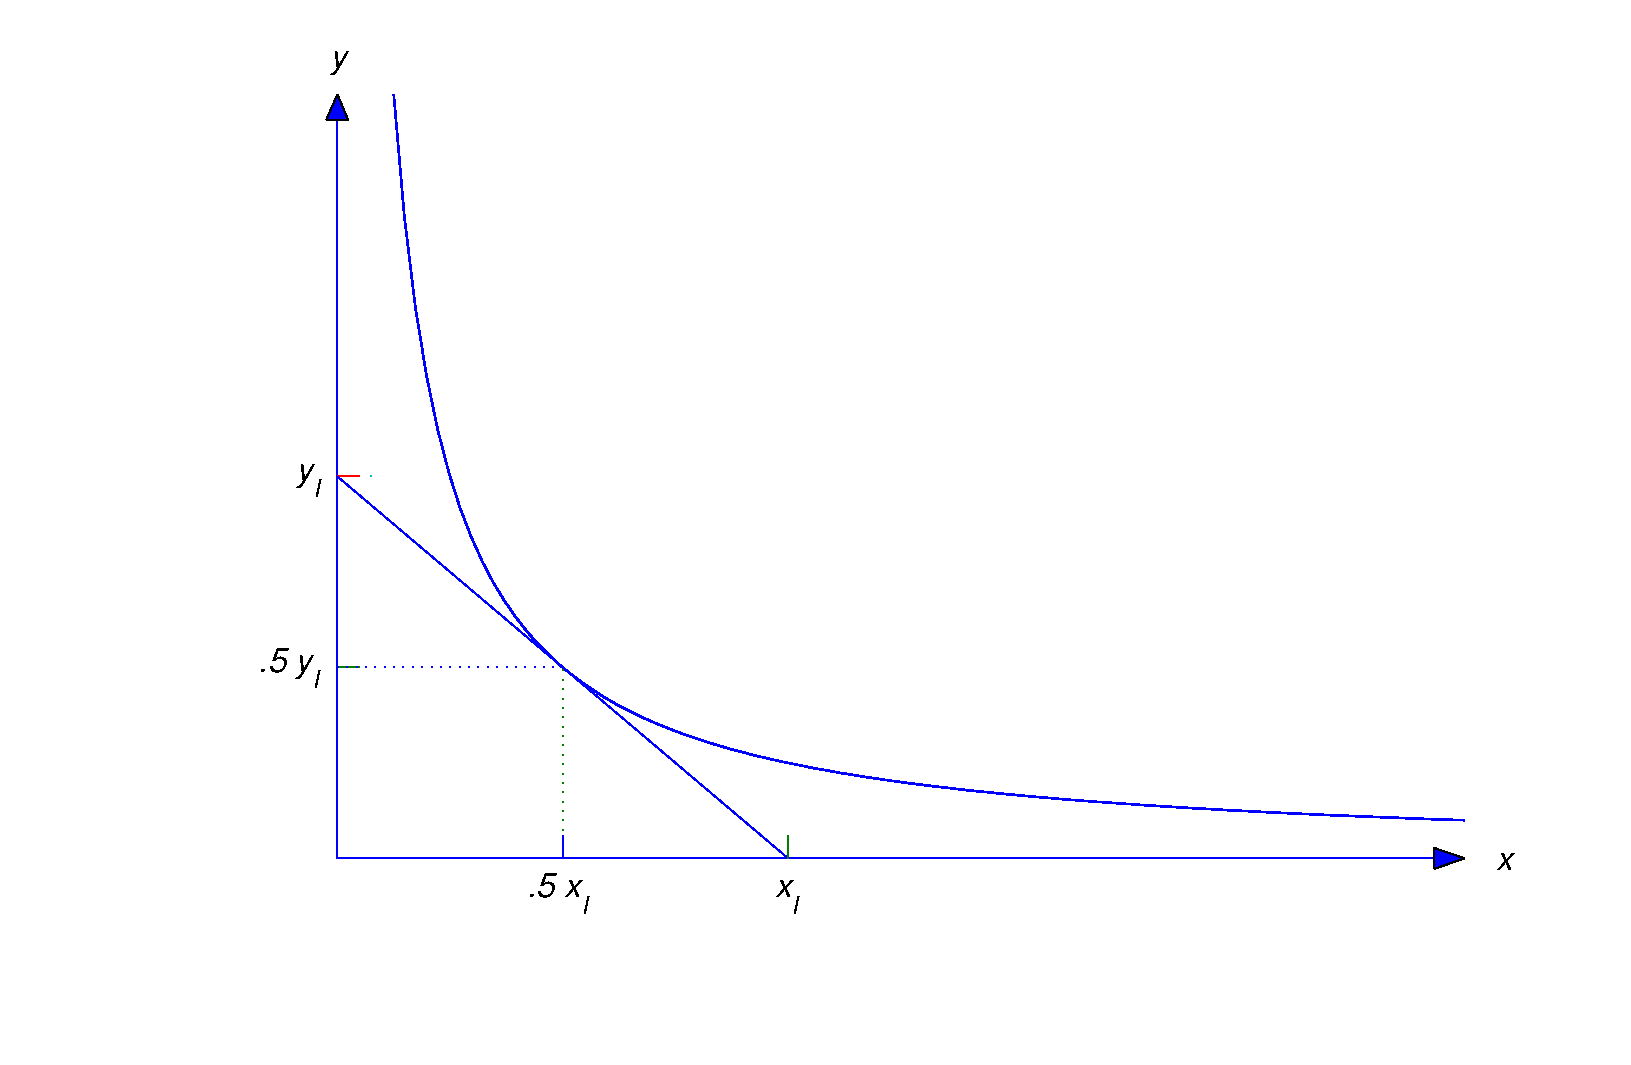
\includegraphics[bb=-78 148 689 643,width=5.67in,height=3.66in,keepaspectratio]{fig040506} }
\caption{}
  \label{figure:4.5.6}
  \end{minipage}
  \hspace{0.6cm}
  \begin{minipage}[b]{0.5\linewidth}
    \centering
   \scalebox{.65}{
  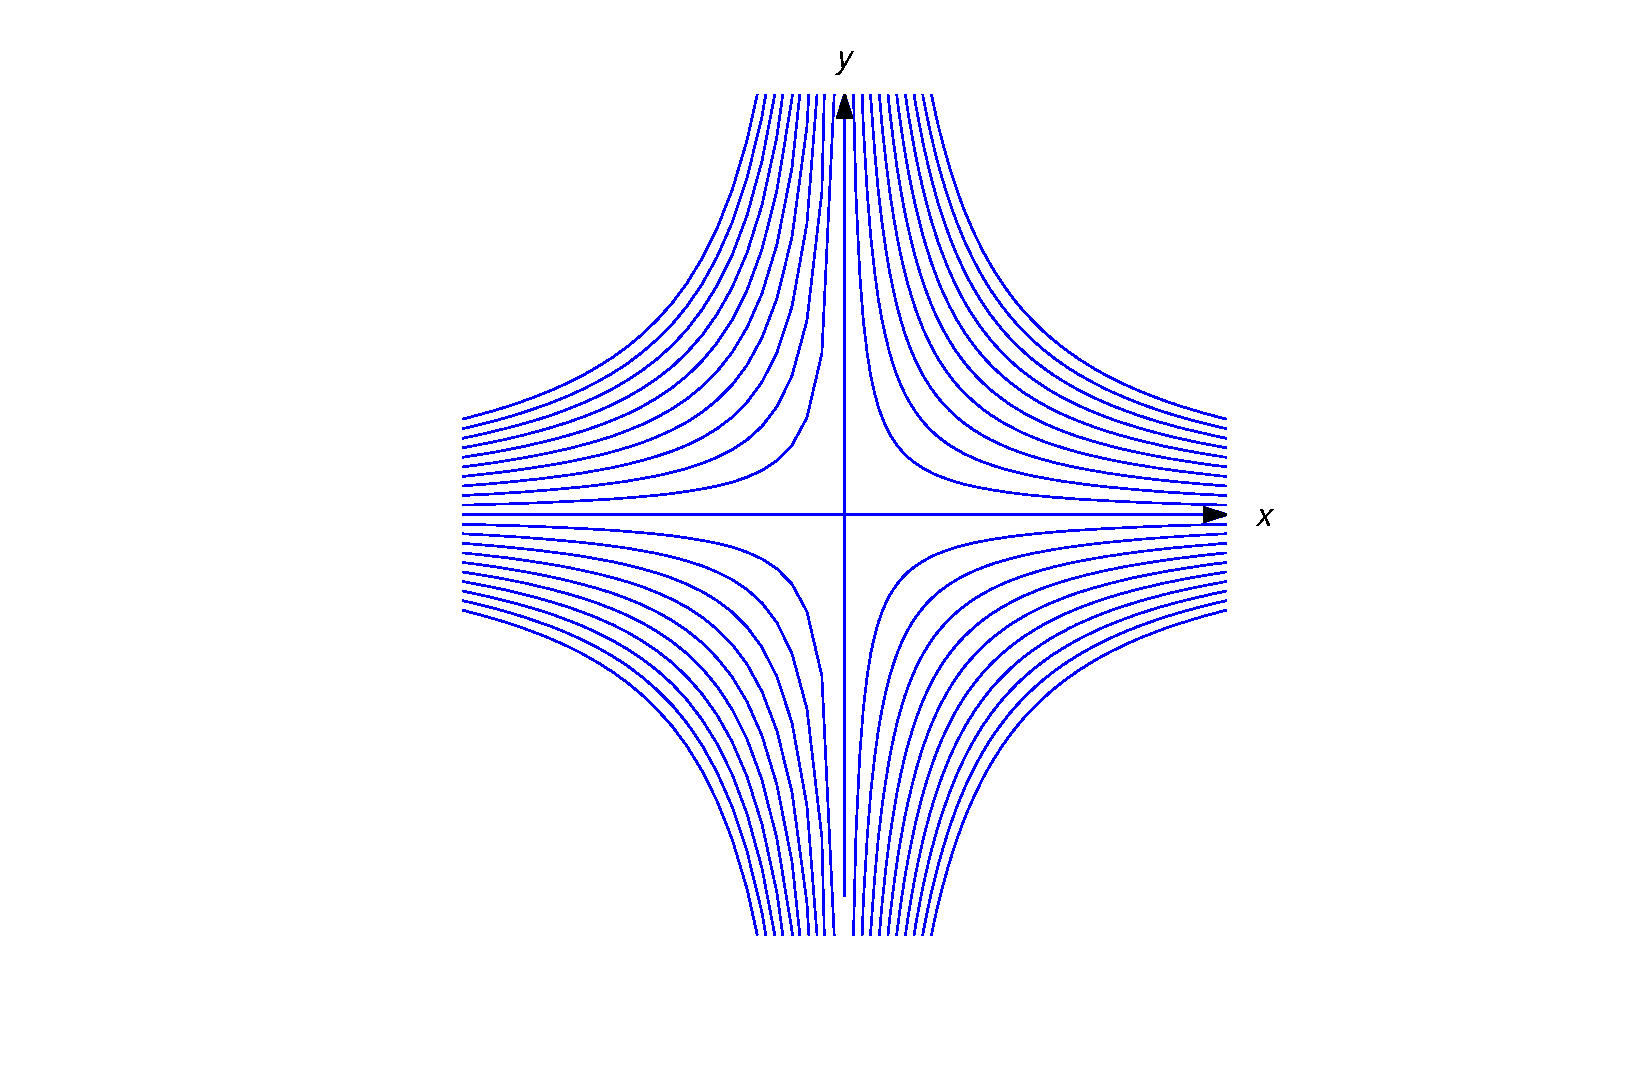
\includegraphics[bb=-78 148 689 643,width=5.67in,height=3.66in,keepaspectratio]{fig040507}}
\caption{}
  \label{figure:4.5.7}
  \end{minipage}
\end{figure}

\begin{example}\label{example:4.5.8}\rm
Find curves $y=y(x)$ such that the tangent line to the curve at any
point $(x_0,y(x_0))$ intersects the $x$-axis at $(x^2_0,0)$.
Figure~\ref{figure:4.5.8} illustrates the situation in the case where
the curve is in the first quadrant and $0<x<1$.
\end{example}

\begin{figure}[htbp]
\color{blue}
  \begin{minipage}[b]{0.5\linewidth}
    \centering
   \scalebox{.65}{
  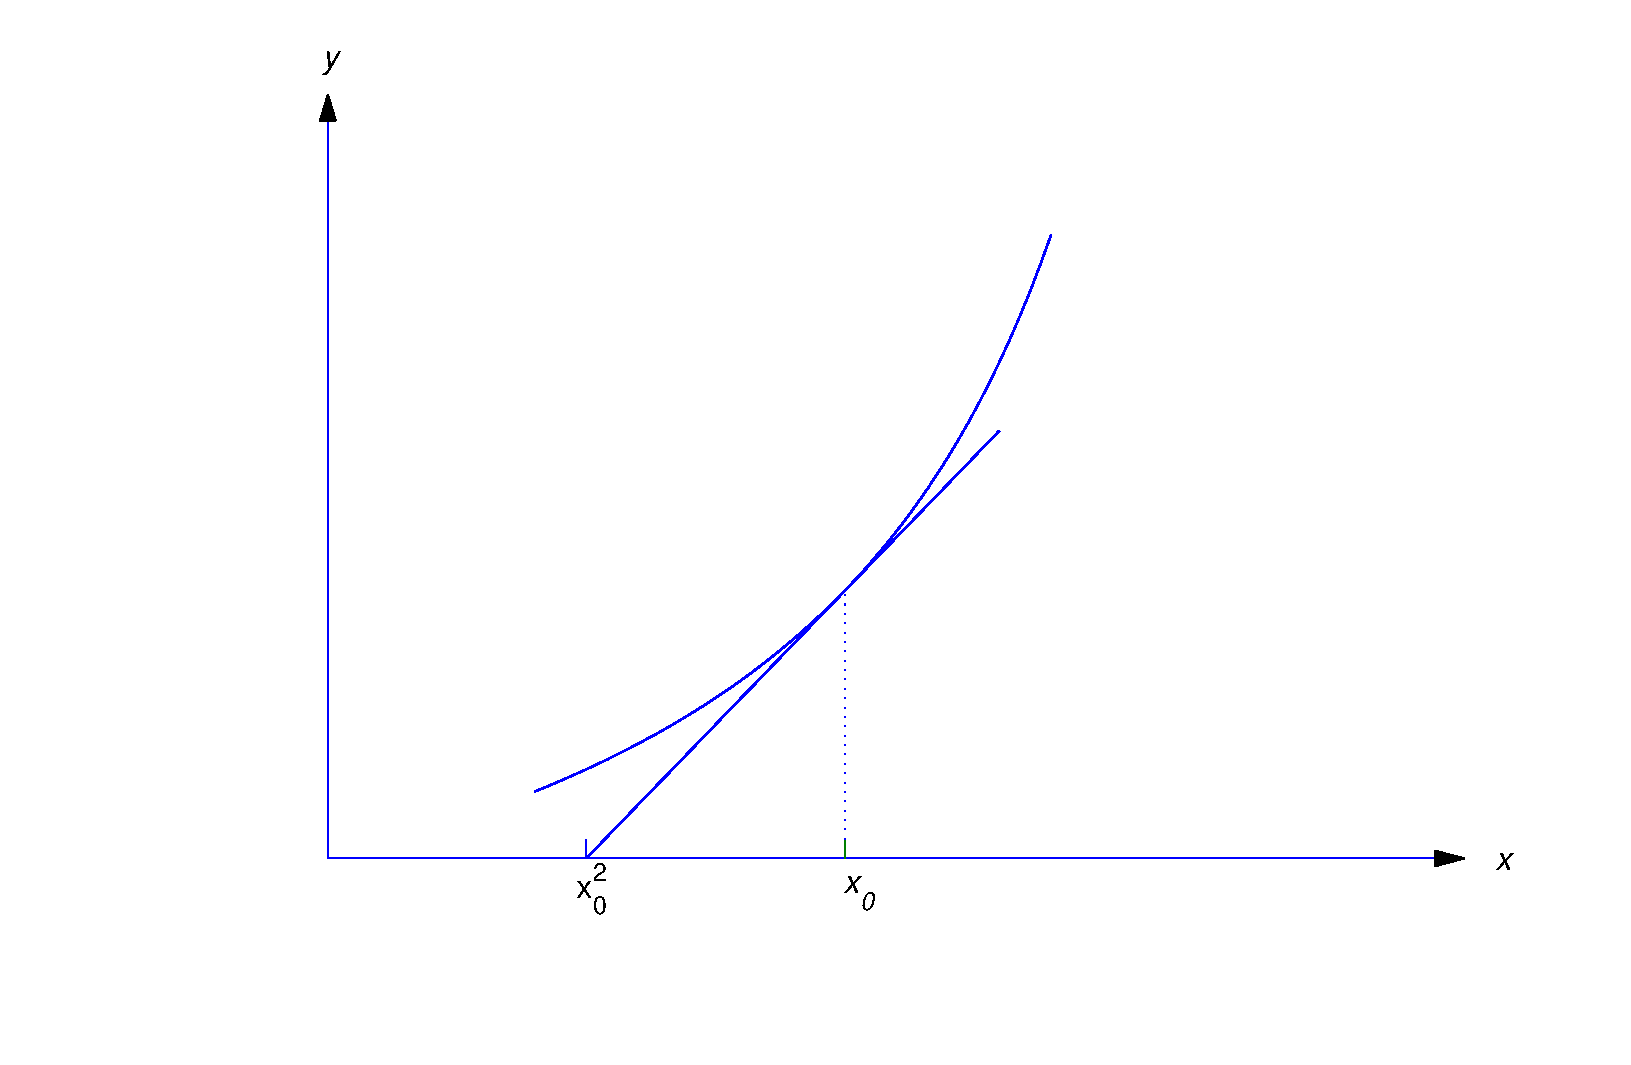
\includegraphics[bb=-78 148 689 643,width=5.67in,height=3.66in,keepaspectratio]{fig040508} }
\caption{}
  \label{figure:4.5.8}
  \end{minipage}
  \hspace{0.6cm}
  \begin{minipage}[b]{0.5\linewidth}
    \centering
   \scalebox{.65}{
  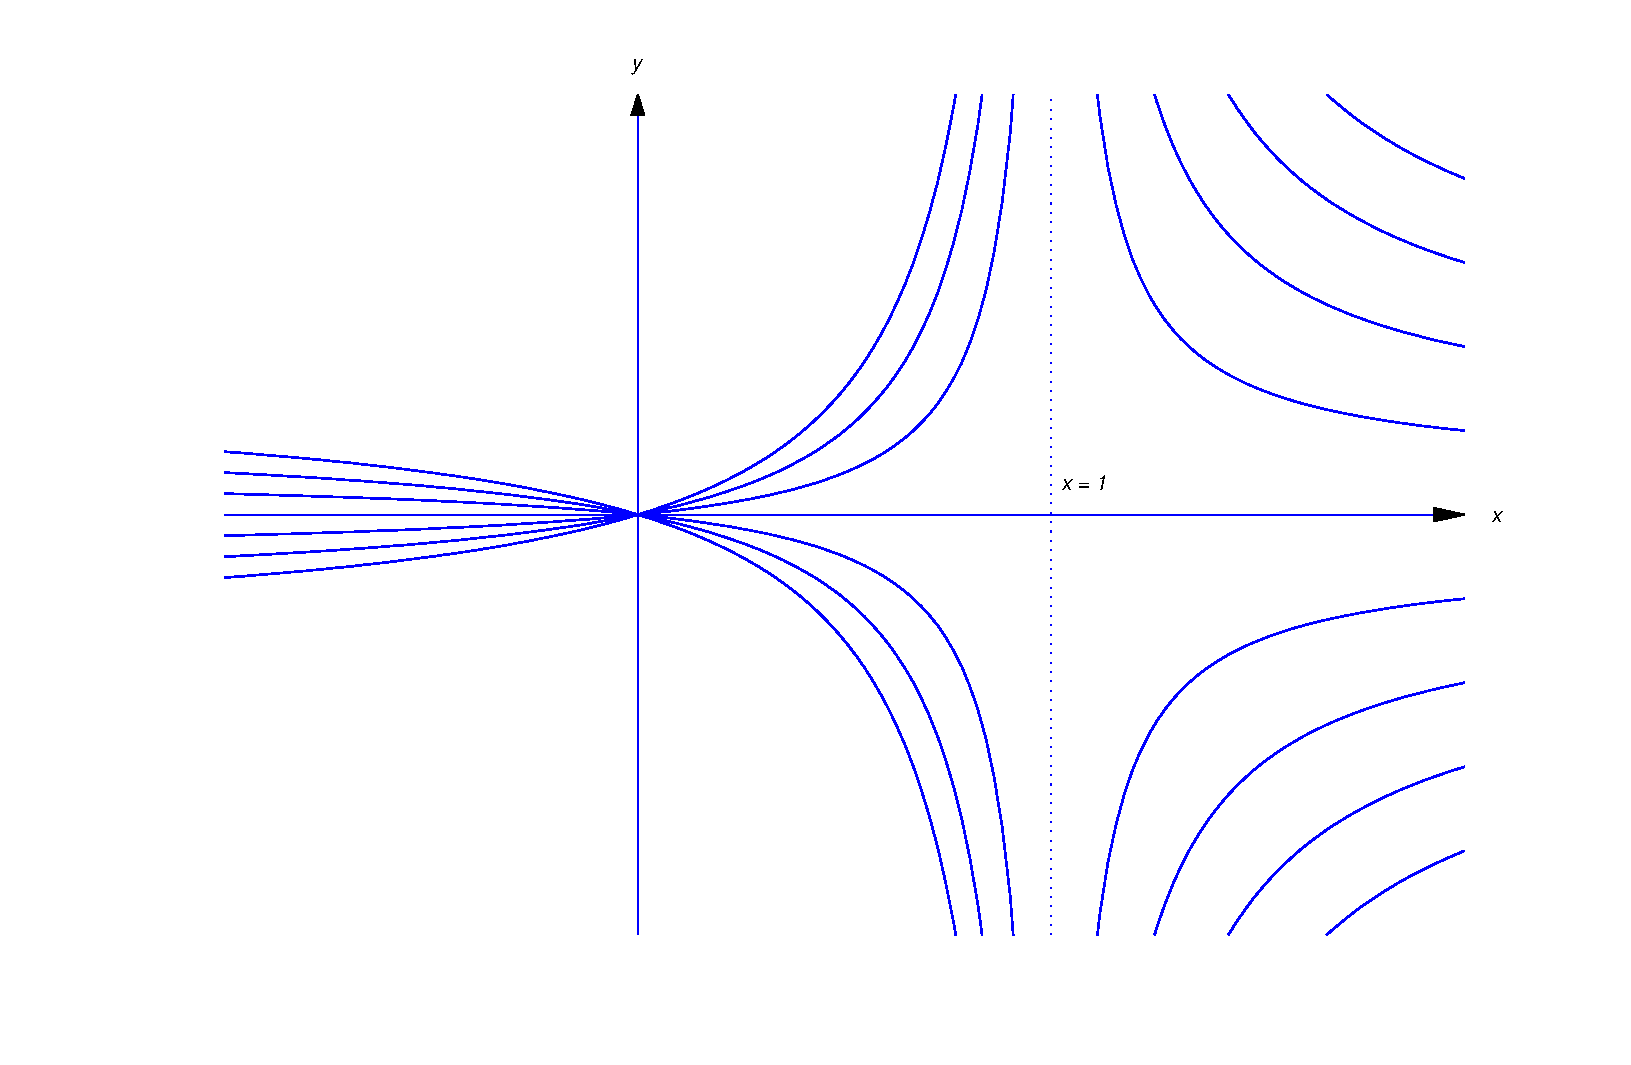
\includegraphics[bb=-78 148 689 643,width=5.67in,height=3.66in,keepaspectratio]{fig040509} }
\caption{}
  \label{figure:4.5.9}
  \end{minipage}
\end{figure}

\solution
The equation of the line tangent to the curve at $(x_0,y(x_0))$ is
$$
y=y(x_0)+y'(x_0)(x-x_0).
$$
Since $(x^2_0,0)$ is on the tangent line,
$$
0=y(x_0)+y'(x_0)(x^2_0-x_0).
$$
Since $x_0$ is arbitrary we drop the subscript and conclude that
$y=y(x)$ satisfies
$$
y+y'(x^2-x)=0.
$$
Therefore
$$
{y'\over y}=-{1\over x^2-x}=-{1\over x(x-1)}={1\over x}-{1\over x-1},
$$
so
$$
\ln|y|=\ln|x|-\ln|x-1|+k=
\ln\left|{x\over x-1}\right|+k,
$$
and
$$
y={cx\over x-1}.
$$
If $c=0$, the graph of this function is the $x$-axis.   If $c\ne0$, it's
a hyperbola with vertical asymptote $x=1$ and horizontal asymptote
$y=c$. Figure~\ref{figure:4.5.9} shows the graphs for $c\ne0$.

\boxit{Orthogonal Trajectories}

\noindent
Two curves $C_1$ and $C_2$ are said to be \it orthogonal \rm at a
point of intersection $(x_0,y_0)$ if they have perpendicular tangents
at $(x_0,y_0)$. (Figure~\ref{figure:4.5.10}). A curve is said to be an
{\color{blue}\it orthogonal trajectory \/} of a given family of curves if it's
orthogonal to every curve in the family. For example, every line
through the origin is an orthogonal trajectory of the family of
circles centered at the origin.  Conversely,
any such circle is an orthogonal trajectory of the family of lines
through the origin (Figure~\ref{figure:4.5.11}).

\begin{figure}[htbp]
\color{blue}
  \begin{minipage}[b]{0.5\linewidth}
    \centering
   \scalebox{.7}{
  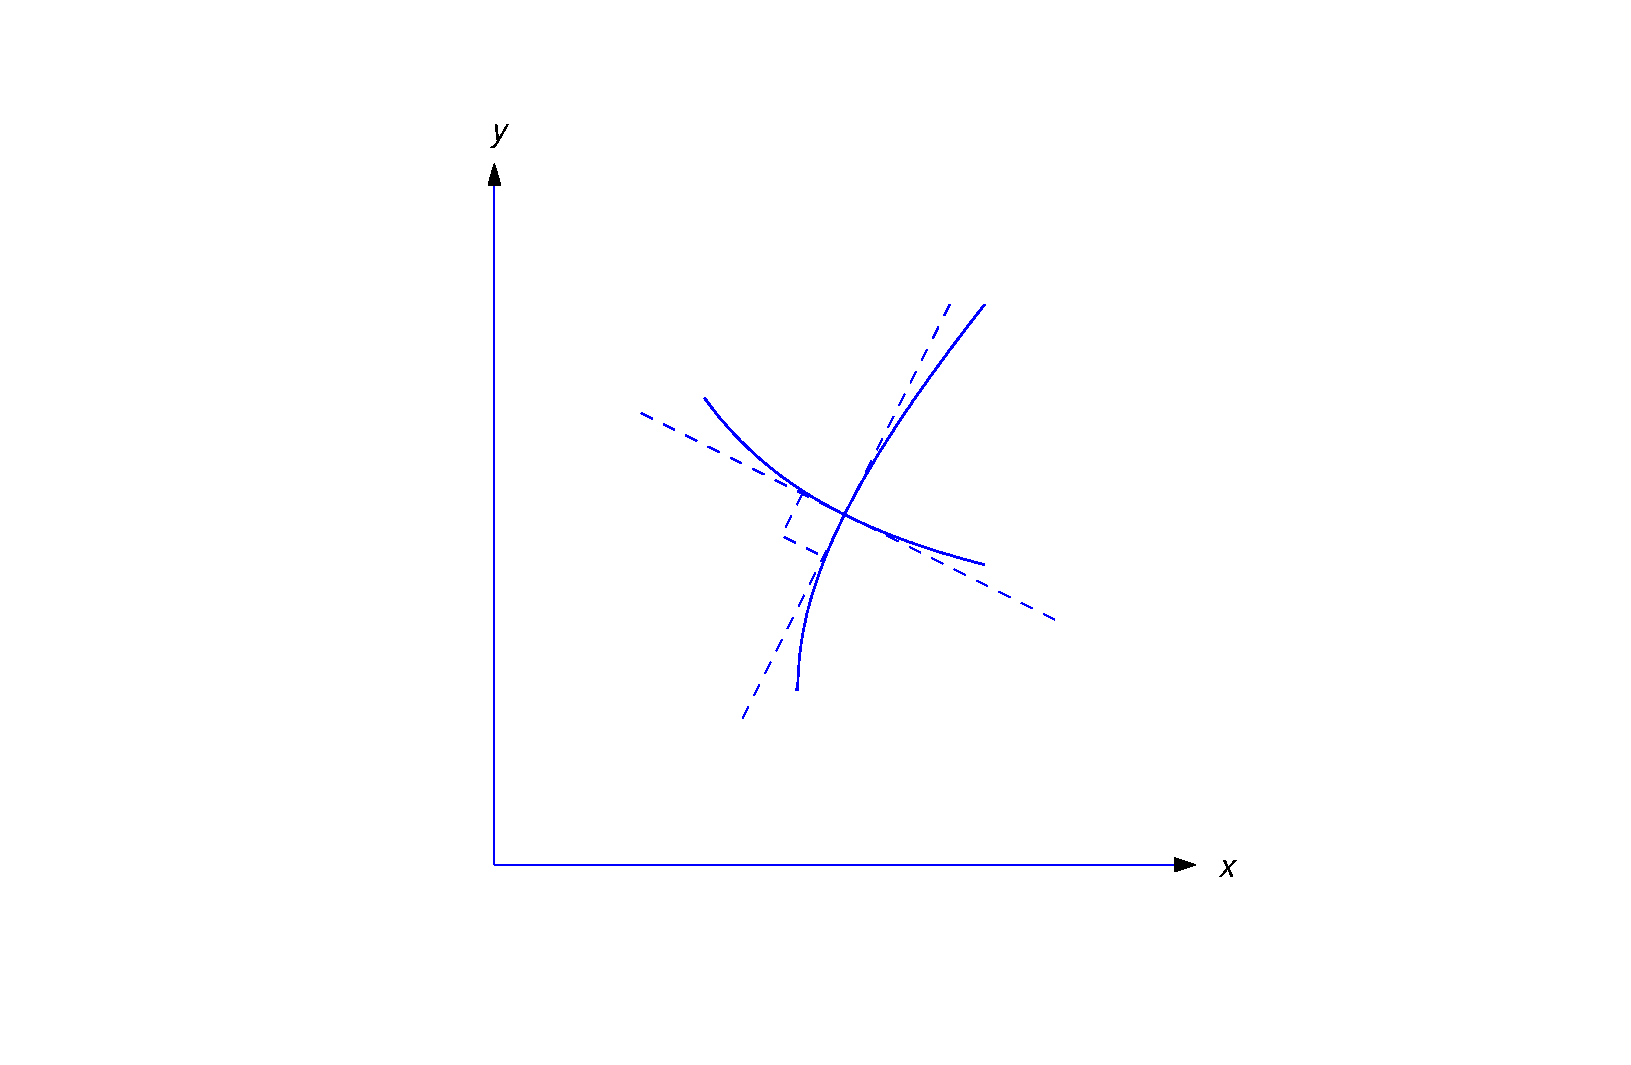
\includegraphics[bb=-78 148 689 643,width=5.67in,height=3.66in,keepaspectratio]{fig040510}}
  \caption{Curves orthogonal at a point of intersection}
  \label{figure:4.5.10}
\end{minipage}
  \begin{minipage}[b]{0.5\linewidth}
    \centering
   \scalebox{.7}{
  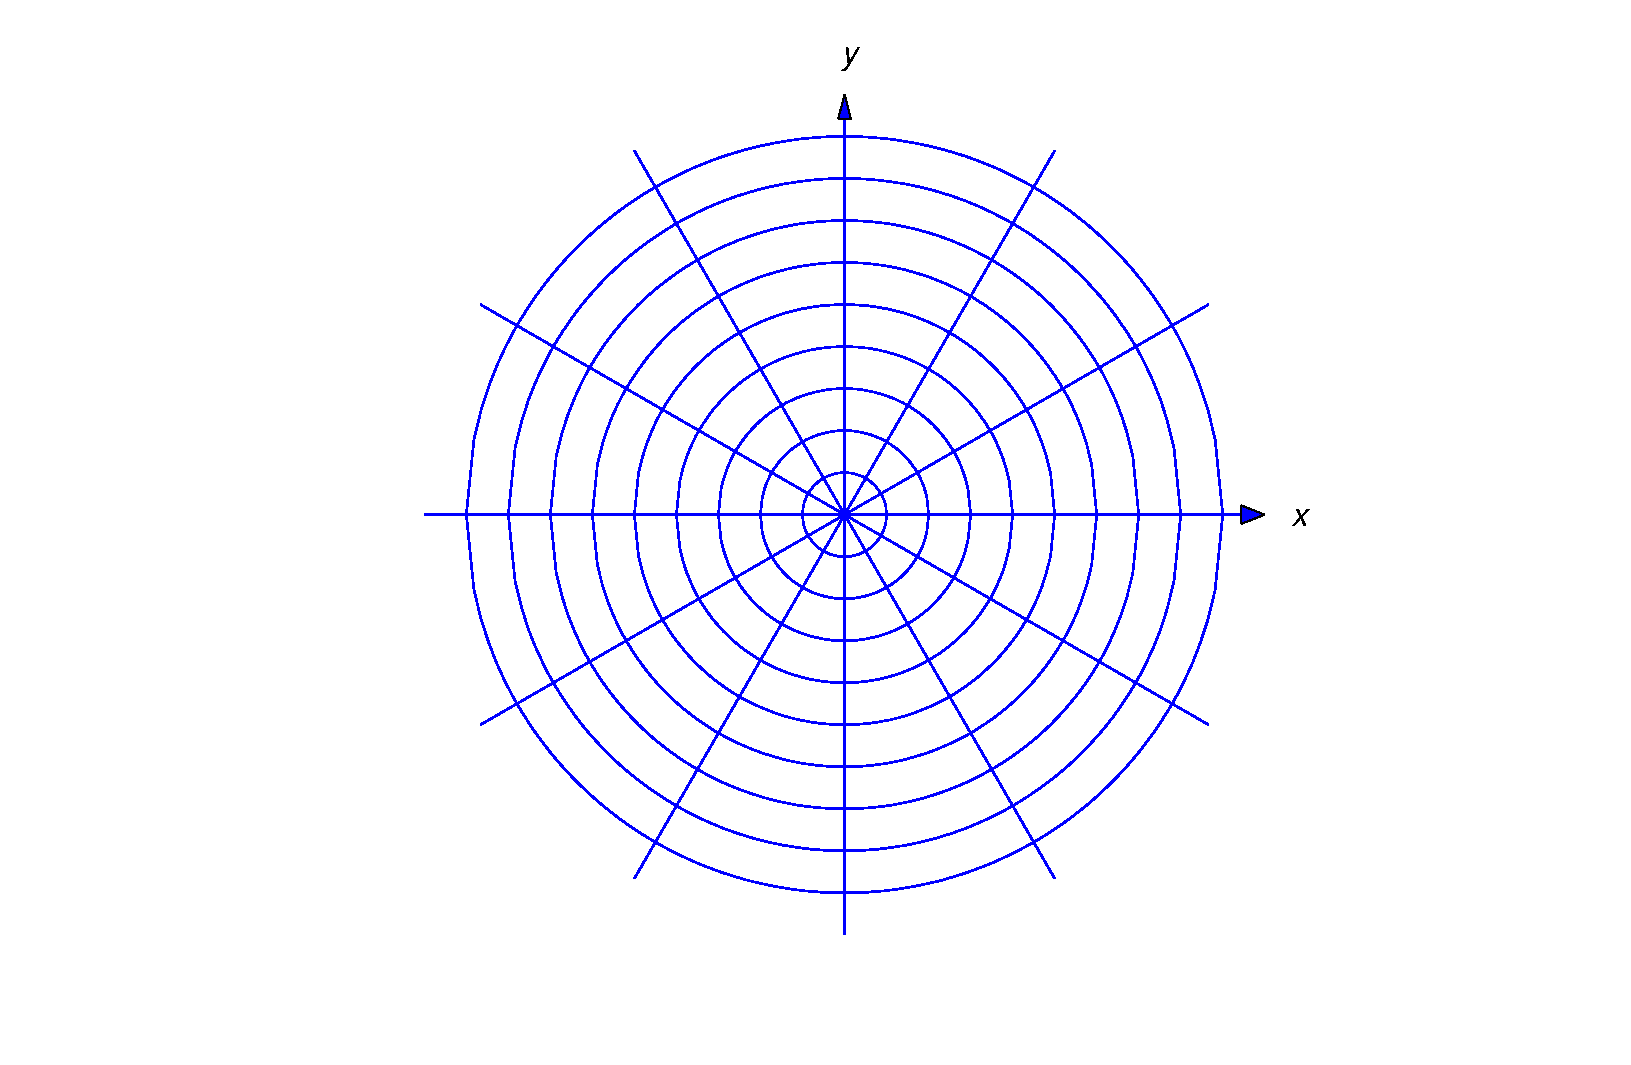
\includegraphics[bb=-78 148 689 643,width=5.67in,height=3.66in,keepaspectratio]{fig040511}}
  \caption{Orthogonal families of circles and lines}
  \label{figure:4.5.11}
\end{minipage}
\end{figure}

Orthogonal trajectories occur in many physical applications.
For example, if $u=u(x,y)$ is the temperature at a point $(x,y)$,  the
curves defined by
\begin{equation} \label{eq:4.5.16}
u(x,y)=c
\end{equation}
are called {\color{blue}\it isothermal\/} curves. The orthogonal trajectories of
this family are called {\color{blue}\it heat-flow\/} lines, because at any given
point the direction of maximum heat flow is perpendicular to the
isothermal through the point. If $u$ represents the potential energy
of an object moving under a force that depends upon $(x,y)$,  the
curves \eqref{eq:4.5.16} are called {\color{blue}\it equipotentials\/}, and the
orthogonal trajectories are called {\color{blue}\it lines of force\/}.

From analytic geometry we know that two nonvertical lines $L_1$ and
$L_2$ with slopes $m_1$ and $m_2$, respectively, are perpendicular if
and only if $m_2=-1/m_1$;  therefore, the integral curves of the
differential equation
$$
y'=-{1\over f(x,y)}
$$
are orthogonal trajectories of the integral curves of the differential
equation
$$
y'=f(x,y),
$$
because at any point $(x_0,y_0)$ where curves from the two families
intersect the slopes of the respective tangent lines are
$$
m_1=f(x_0,y_0)\mbox{\quad and \quad} m_2=-{1\over f(x_0,y_0)}.
$$

This suggests a  method for finding orthogonal trajectories
of a family of integral curves of a first order equation.

\boxit{Finding Orthogonal Trajectories}

{\bf Step 1.} Find a differential equation
$$
y'=f(x,y)
$$
 for the given family.

\medskip

{\bf Step 2.} Solve the differential equation
$$
y'=-{1\over f(x,y)}
$$
to find the orthogonal trajectories.

\begin{example}\label{example:4.5.9} \rm
Find the orthogonal trajectories of the family of circles
\begin{equation} \label{eq:4.5.17}
x^2+y^2=c^2 \quad (c>0).
\end{equation}
\end{example}

\solution
To find a differential equation for the family of circles we
differentiate \eqref{eq:4.5.17} implicitly with respect to $x$ to obtain
$$
2x+2yy'=0,
$$
or
$$
y'=-{x\over y}.
$$
Therefore the integral curves  of
$$
y'={y\over x}
$$
are orthogonal trajectories of the given family. We leave it to you to
verify that the general solution of this equation is
$$
y=kx,
$$
where $k$ is an arbitrary constant. This is the equation of a
nonvertical line through $(0,0)$. The $y$ axis is also an orthogonal
trajectory of the given family. Therefore every line through the
origin is an orthogonal trajectory of the given family \eqref{eq:4.5.17}
(Figure~\ref{figure:4.5.11}). This is consistent with the theorem of plane
geometry which states that a diameter of a circle and a tangent line
to the circle at the end of the diameter are perpendicular.

\begin{example}\label{example:4.5.10} \rm
Find the orthogonal trajectories of the family of hyperbolas
\begin{equation}  \label{eq:4.5.18}
xy=c \quad (c\ne0)
\end{equation}
(Figure~\ref{figure:4.5.7}).
\end{example}

\solution
Differentiating \eqref{eq:4.5.18} implicitly with respect to $x$ yields
$$
y+xy'=0,
$$
or
$$
y'=-{y\over x};
$$
 thus, the integral curves of
$$
y'={x\over y}
$$
are orthogonal trajectories of the given family. Separating variables
yields
$$
y'y=x
$$
and integrating yields
$$
y^2-x^2=k,
$$
which is the equation of a hyperbola if $k \ne0$, or of the lines
$y=x$ and $y=-x$ if $k=0$ (Figure~\ref{figure:4.5.12}).

\begin{figure}[tbp]
  \centering
  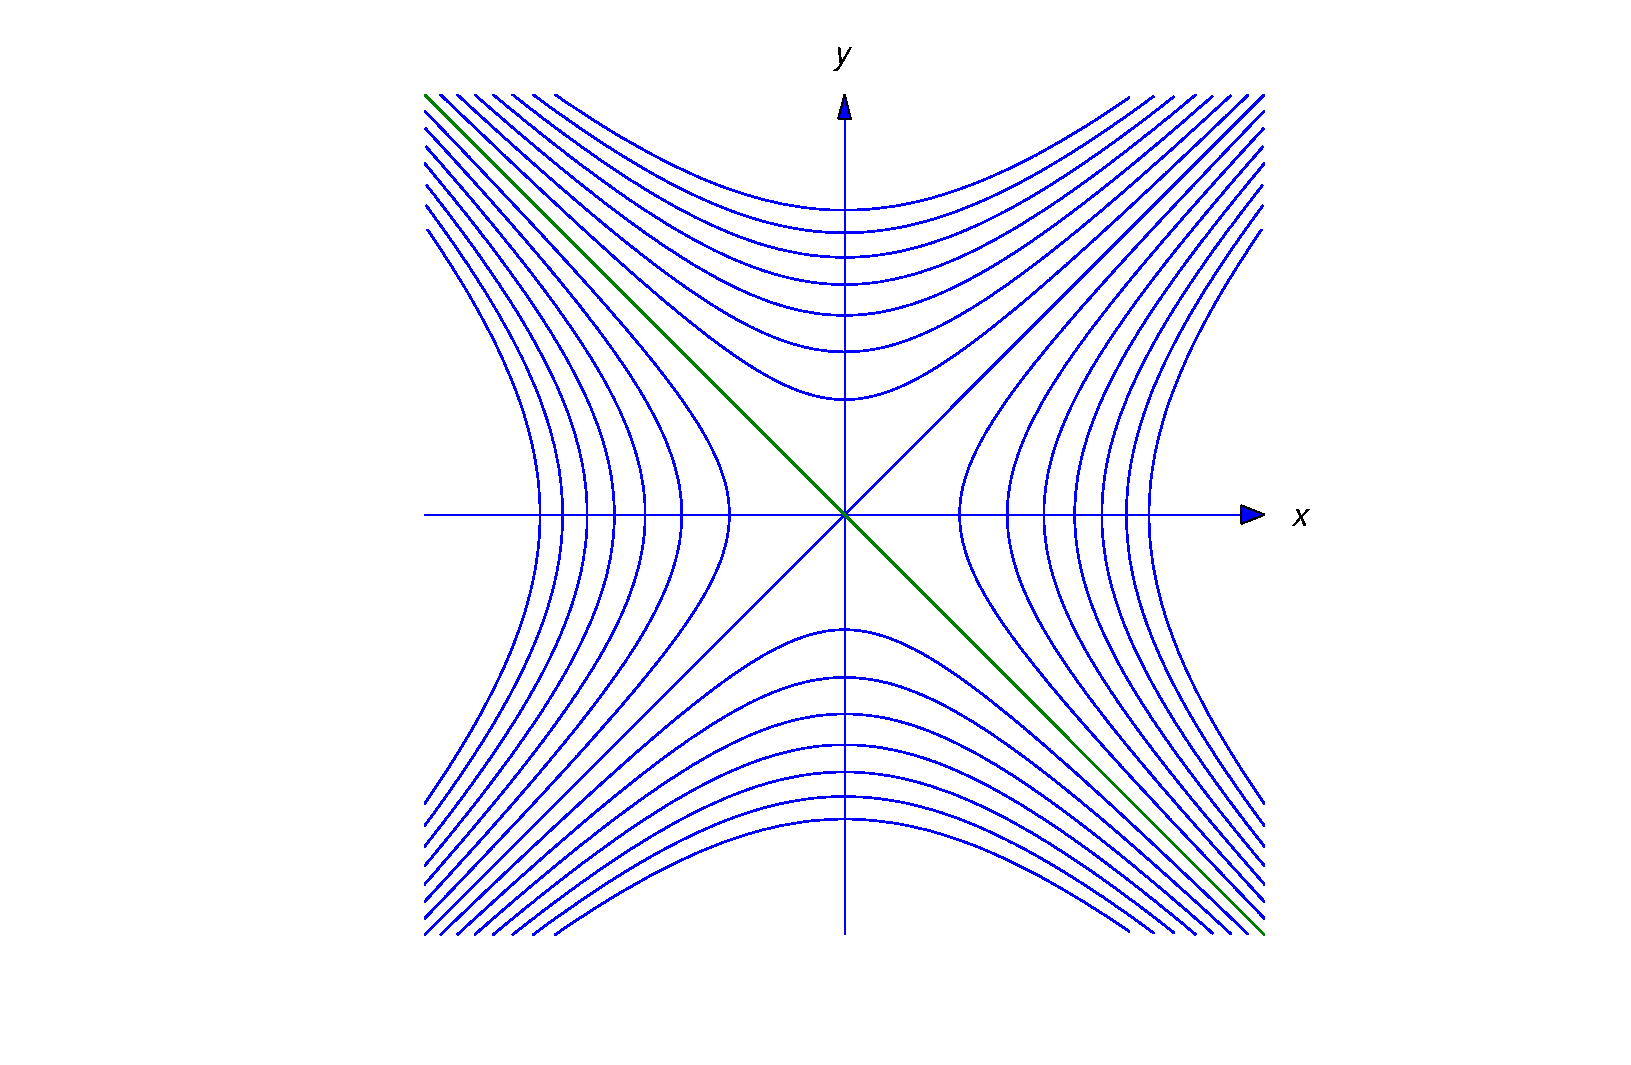
\includegraphics[bb=-78 148 689 643,width=5.67in,height=3.66in,keepaspectratio]{fig040512}
\color{blue}
\caption{ Orthogonal trajectories of the hyperbolas $xy=c$}
  \label{figure:4.5.12}
\end{figure}

\begin{example}\rm
Find the orthogonal trajectories of the family of circles defined by
\begin{equation} \label{eq:4.5.19}
(x-c)^2+y^2=c^2 \quad (c\ne0).
\end{equation}
 These circles are centered on the $x$-axis and tangent to the
$y$-axis (Figure~\ref{figure:4.5.13}\part{a}).
\end{example}

\solution
Multiplying out the left side of \eqref{eq:4.5.19} yields
\begin{equation} \label{eq:4.5.20}
x^2-2cx+y^2=0,
\end{equation}
and differentiating this implicitly with respect to $x$ yields
\begin{equation} \label{eq:4.5.21}
2(x-c)+2yy'=0.
\end{equation}
 From \eqref{eq:4.5.20},
$$
c={x^2+y^2\over2x},
$$
so
$$
x-c=x-{x^2+y^2\over2x}={x^2-y^2\over2x}.
$$
Substituting this into \eqref{eq:4.5.21} and solving for $y'$ yields
\begin{equation} \label{eq:4.5.22}
y'={y^2-x^2\over2xy}.
\end{equation}
The curves defined by \eqref{eq:4.5.19} are integral curves of
\eqref{eq:4.5.22}, and the integral curves of
$$
y'={2xy\over x^2-y^2}
$$
are orthogonal trajectories of the family \eqref{eq:4.5.19}. This is a
homogeneous nonlinear equation, which we studied in
Section~2.4. Substituting $y=ux$ yields
$$
u'x+u={2x(ux)\over x^2-(ux)^2}={2u\over1-u^2},
$$
so
$$
u'x={2u\over1-u^2}-u={u(u^2+1)\over1-u^2},
$$
Separating variables yields
$$
{1-u^2\over u(u^2+1)}u'={1\over x},
$$
or, equivalently,
$$
\left[{1\over u}-{2u\over u^2+1}\right]u'={1\over x}.
$$
Therefore
$$
\ln |u|-\ln (u^2+1)=\ln |x|+k.
$$
By substituting $u=y/x$, we see that
$$
\ln|y|-\ln|x|-\ln(x^2+y^2)+\ln(x^2)=\ln|x|+k,
$$
which, since $\ln(x^2)=2\ln|x|$, is equivalent to
$$
\ln|y|-\ln(x^2+y^2)=k,
$$
or
$$
|y|=e^k(x^2+y^2).
$$
To see what these curves are we rewrite this equation as
$$
x^2+|y|^2-e^{-k}|y|=0
$$
and complete the square to obtain
$$
x^2+(|y|-e^{-k}/2)^2=(e^{-k}/2)^2.
$$
This can be rewritten as
$$
x^2+(y-h)^2=h^2,
$$
where
$$
h=\left\{\begin{array}{rl} \dst{e^{-k}\over2}&\mbox{ if } y\ge
0,\\[\jot]-\dst{e^{-k}\over2}&\mbox{ if } y\le0. \end{array}\right.
$$
Thus, the orthogonal trajectories are circles centered on the $y$ axis
and tangent to the $x$ axis (Figure~\ref{figure:4.5.13}(b)). The circles
for which $h>0$ are above the $x$-axis, while those for which $h<0$
are below.

\enlargethispage{2in}

\begin{figure}[H]
  \centering
\scalebox{.9}{
  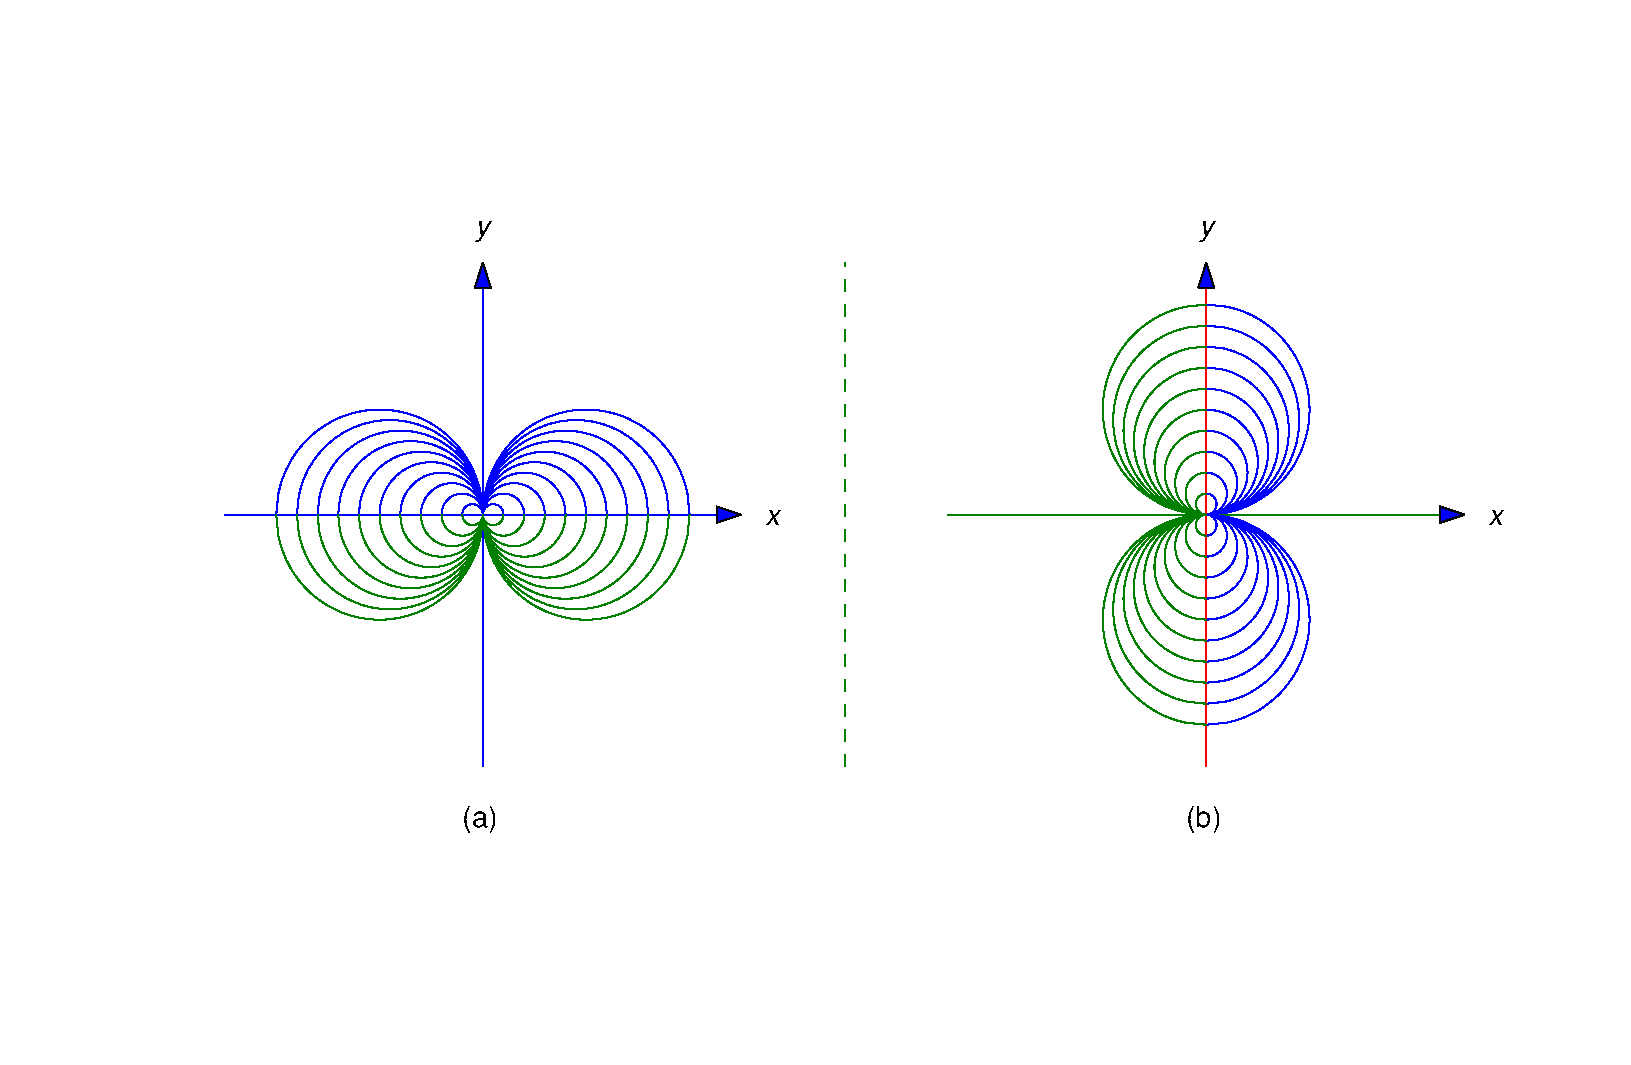
\includegraphics[bb=-78 148 689 643,width=5.67in,height=3.66in,keepaspectratio]{fig040513}}
\color{blue}
\caption{{\bf (a)} The circles $(x-c)^2+y^2=c^2$ \, {\bf (b)} The circles
$x^2+(y-h)^2=h^2$}
\vspace*{-40pt}
  \label{figure:4.5.13}
\end{figure}

\newpage

\exercises
In  Exercises \ref{exer:4.5.1}--\ref{exer:4.5.8} find a first order
differential equation for the given family of curves.

\begin{exerciselist}

\begin{tabular}[t]{@{}p{168pt}@{}p{168pt}}
\item\label{exer:4.5.1} $y(x^2+y^2)=c$
&\vspace*{10pt}\item\label{exer:4.5.2} $e^{xy}=cy$
\end{tabular}

\begin{tabular}[t]{@{}p{168pt}@{}p{168pt}}
 \item\label{exer:4.5.3} $\ln |xy|=c(x^2+y^2)$&
 \item\label{exer:4.5.4} $y=x^{1/2}+cx$
\end{tabular}

\begin{tabular}[t]{@{}p{168pt}@{}p{168pt}}
\item\label{exer:4.5.5} $y=e^{x^2}+ce^{-x^2}$&
 \item\label{exer:4.5.6} $\dst{y=x^3+{c\over x}}$
\end{tabular}

\begin{tabular}[t]{@{}p{168pt}@{}p{168pt}}
\item\label{exer:4.5.7} $y=\sin x+ce^x$&
\item\label{exer:4.5.8} $y=e^x+c(1+x^2)$
\end{tabular}

\item\label{exer:4.5.9}
Show that the family of circles
$$
(x-x_0)^2+y^2=1,\;-\infty<x_0<\infty,
$$
can be obtained by joining integral curves of two first order
differential equations. More specifically, find differential equations
for the families of semicircles
$$
(x-x_0)^2+y^2=1,\; x_0<x<x_0+1,\;-\infty<x_0<\infty,
$$
$$
(x-x_0)^2+y^2=1,\; x_0-1<x<x_0,\;-\infty<x_0<\infty.
$$

\item\label{exer:4.5.10}
Suppose $f$ and $g$ are differentiable for all $x$. Find a
differential equation for the family of functions $y=f+cg$
($c$=constant).

\exercisetext{In Exercises \ref{exer:4.5.11}--\ref{exer:4.5.13} find a
first order differential equation for the given family of curves.}

\item\label{exer:4.5.11}
Lines through a given point $(x_0,y_0)$.

\item\label{exer:4.5.12}
Circles through $(-1,0)$ and $(1,0)$.

\item\label{exer:4.5.13}
Circles through $(0,0)$ and $(0,2)$.

\item\label{exer:4.5.14}
Use the method Example~\ref{example:4.5.6}{\bf (a)} to find the equations
of lines through the given points tangent to the parabola $y=x^2$.
Also, find the points of tangency.

\begin{tabular}[t]{@{}p{78pt}@{}p{78pt}p{78pt}p{78pt}}
{\bf (a)}\; $(5,9)$
&{\bf (b)}\; $(6,11)$
&{\bf (c)}\; $(-6,20)$
&{\bf (d)}\; $(-3,5)$
\end{tabular}

\item\label{exer:4.5.15}
\begin{alist}
\item % (a)
Show that the equation of the line tangent to the circle
$$
x^2+y^2=1
\eqno{\rm (A)}
$$
at a point $(x_0,y_0)$  on the circle is
$$
y=\dst{1-x_0x\over y_0}\mbox{\quad if \quad} x_0\ne\pm1.
\eqno{\rm (B)}
$$
\item % (b)
Show that if $y'$ is the slope of a nonvertical tangent line to the
circle (A) and $(x,y)$ is a point on the tangent line then
$$
(y')^2(x^2-1)-2xyy'+y^2-1=0.
\eqno{\rm (C)}
$$
\item % (c)
Show that the segment of the tangent line (B) on which $(x-x_0)/y_0>0$
is an integral curve of the differential equation
$$
y'={xy-\sqrt{x^2+y^2-1}\over x^2-1},
\eqno{\rm (D)}
$$
while the segment on which $(x-x_0)/y_0<0$ is an integral curve of the
differential equation
$$
y'={xy+\sqrt{x^2+y^2-1}\over x^2-1}.
\eqno{\rm (E)}
$$

\hint{Use the quadratic formula to solve ${\rm (C)}$ for
$y'$. Then substitute {\rm (B)} for $y$ and
 choose the $\pm$ sign in the quadratic formula so that the
resulting expression for $y'$ reduces to the known slope
$y'=-x_0/y_0$.}

\item % (d)
Show that the upper and lower semicircles of (A) are also integral
curves of (D) and (E).

\item % (e)
Find the equations of two lines through (5,5) tangent to the circle
(A), and find the points of tangency.
\end{alist}

\item\label{exer:4.5.16}
\begin{alist}
\item % (a)
Show that the equation of the line tangent to the  parabola
$$
x=y^2
\eqno{\rm (A)}
$$
at a point $(x_0,y_0)\ne(0,0)$  on the parabola is
$$
y=\dst{y_0\over2}+\dst{x\over2y_0}.
\eqno{\rm (B)}
$$
\item % (b)
Show that if $y'$ is the slope of a nonvertical tangent line
to the parabola (A) and $(x,y)$ is a point on the tangent
line then
$$
4x^2(y')^2-4xyy'+x=0.
\eqno{\rm (C)}
$$
\item % (c)
Show that the segment of the tangent line defined in \part{a} on which
$x>x_0$ is an integral curve of the differential equation
$$
y'={y+\sqrt{y^2-x}\over2x},
\eqno{\rm (D)}
$$
while the segment on which $x<x_0$ is an integral curve of the
differential equation
$$
y'={y-\sqrt{y^2-x}\over2x},
\eqno{\rm (E)}
$$

\hint{Use the quadratic formula to solve ${\rm (C)}$ for $y'$. Then
substitute {\rm (B)} for $y$ and choose the $\pm$ sign in the
quadratic formula so that the resulting expression for $y'$ reduces to
the known slope $y'=\dst{1\over2y_0}$.}

\item % (d)
Show that the upper and lower halves of the parabola (A), given by
$y=\sqrt x$ and $y=-\sqrt x$ for $x>0$, are also integral curves of
(D) and (E).
\end{alist}

\item\label{exer:4.5.17}
Use the results of Exercise \ref{exer:4.5.16} to find the equations of two
lines tangent to the parabola $x=y^2$ and passing through the given
point. Also find the points of tangency.

\begin{tabular}[t]{@{}p{78pt}@{}p{78pt}p{78pt}p{78pt}}
{\bf (a)}\; $(-5,2)$
&{\bf (b)}\; $(-4,0)$
&{\bf (c)}\; $(7,4)$
&{\bf (d)}\; $(5,-3)$
\end{tabular}

\item\label{exer:4.5.18}
Find a curve $y=y(x)$ through (1,2) such that the tangent to the curve
at any point $(x_0,y(x_0))$ intersects the $x$ axis at
$\dst{x_I=x_0/2}$.

\item\label{exer:4.5.19}
Find all curves $y=y(x)$ such that the tangent to the curve at any
point $(x_0,y(x_0))$ intersects the $x$ axis at $x_I=x^3_0$.

\item\label{exer:4.5.20}
Find all curves $y=y(x)$ such that the tangent to the curve at any
point passes through a given point $(x_1,y_1)$.

\item\label{exer:4.5.21}
Find a curve $y=y(x)$ through $(1,-1)$ such that the tangent to the
curve at any point $(x_0,y(x_0))$ intersects the $y$ axis at
$y_I=x^3_0$.

\item\label{exer:4.5.22}
Find all curves $y=y(x)$ such that the tangent to the curve at any
point $(x_0,y(x_0))$ intersects the $y$ axis at $y_I=x_0$.

\item\label{exer:4.5.23}
Find a curve $y=y(x)$ through $(0,2)$ such that the normal to the
curve at any point $(x_0,y(x_0))$ intersects the $x$ axis at
$x_I=x_0+1$.

\item\label{exer:4.5.24}
Find a curve $y=y(x)$ through $(2,1)$ such that the normal to the
curve at any point $(x_0,y(x_0))$ intersects the $y$ axis at
$y_I=2y(x_0)$.

\exercisetext{In Exercises \ref{exer:4.5.25}--\ref{exer:4.5.29} find the
orthogonal trajectories of the given family of curves.}

\begin{tabular}[t]{@{}p{168pt}@{}p{168pt}}
\item\label{exer:4.5.25} $x^2+2y^2=c^2$
&\vspace*{10pt}\item\label{exer:4.5.26} $x^2+4xy+y^2=c$
\end{tabular}

\begin{tabular}[t]{@{}p{168pt}@{}p{168pt}}
\item\label{exer:4.5.27} $y=ce^{2x}$
&\item\label{exer:4.5.28} $xye^{x^2}=c$
\end{tabular}

\item\label{exer:4.5.29}
$\dst{y={ce^x\over x}}$

\item\label{exer:4.5.30}
Find a curve through $(-1,3)$ orthogonal to every parabola of the form
$$
y=1+cx^2
$$
that it intersects. Which of these parabolas does the desired curve
intersect?

\item\label{exer:4.5.31}
Show that the orthogonal trajectories of
$$
x^2+2axy+y^2=c
$$
satisfy
$$
|y-x|^{a+1}|y+x|^{a-1}=k.
$$

\item\label{exer:4.5.32}
If lines $L$ and $L_1$ intersect at $(x_0,y_0)$ and $\alpha$ is the
smallest angle through which $L$ must be rotated counterclockwise
about $(x_0,y_0)$ to bring it into coincidence with $L_1$, we say that
$\alpha$ is the {\color{blue}\it angle from $L$ to $L_1$\/};   thus,
$0\le\alpha<\pi$. If $L$ and $L_1$ are tangents to curves $C$ and
$C_1$, respectively, that intersect at $(x_0,y_0)$, we say that $C_1$
intersects $C$ at the angle $\alpha$. Use the identity
$$
\tan(A+B)={\tan A+\tan B\over1-\tan A\tan B}
$$
to show that if $C$ and $C_1$ are intersecting integral curves of
$$
y'=f(x,y)  \mbox{\quad and \quad} y'={f(x,y)+\tan\alpha\over
1-f(x,y)\tan\alpha} \quad\left( \alpha \ne {\pi\over2}\right),
$$
respectively, then $C_1$ intersects $C$ at the angle $\alpha$.

\item\label{exer:4.5.33}
Use the result of Exercise~\ref{exer:4.5.32} to find a family of curves
that intersect every nonvertical line through the origin at the angle
$\alpha=\pi/4$.

\item\label{exer:4.5.34}
Use the result of Exercise~\ref{exer:4.5.32} to find a family of curves
that intersect every circle centered at the origin at a given angle
$\alpha \ne \pi/2$.

\end{exerciselist}


